\RequirePackage[l2tabu,orthodox]{nag}

\documentclass[11pt,a4paper,twoside]{memoir}
\usepackage[utf8]{inputenc}

\usepackage{amsmath}
%\usepackage{amsfonts}
%\usepackage{amssymb}
\usepackage{amsthm}
\usepackage{mathtools}

%\usepackage{lmodern}
%\usepackage{slantsc}
%\usepackage{fourier}
%\usepackage{tgschola}
\usepackage[bitstream-charter]{mathdesign}
%\usepackage[libertine]{newtxmath}

%\usepackage{polyglossia}
%\setdefaultlanguage{english}
\usepackage[english]{babel}
\usepackage{csquotes}

\frenchspacing
\nonzeroparskip
\setlength\parskip{0.58\parskip}

\usepackage[style=authoryear-icomp,maxbibnames=99,dashed=false,maxcitenames=2,uniquelist=false,backref=true,backend=biber]{biblatex}

\setlength\bibitemsep{\parskip}

\usepackage[activate={true,nocompatibility},final,tracking=true,kerning=true,spacing=true,factor=1100,stretch=10,shrink=10]{microtype}
%\usepackage[activate={true,nocompatibility},final,tracking=true,factor=1100,stretch=10,shrink=10]{microtype}
\SetProtrusion{encoding={*},family={bch},series={*},size={6,7}}
              {1={ ,750},2={ ,500},3={ ,500},4={ ,500},5={ ,500},
               6={ ,500},7={ ,600},8={ ,500},9={ ,500},0={ ,500}}
\SetExtraKerning[unit=space]
    {encoding={*}, family={bch}, series={*}, size={footnotesize,small,normalsize}}
    {\textendash={400,400}, % en-dash, add more space around it
     "28={ ,150}, % left bracket, add space from right
     "29={150, }, % right bracket, add space from left
     \textquotedblleft={ ,150}, % left quotation mark, space from right
     \textquotedblright={150, }} % right quotation mark, space from left
\SetExtraKerning[unit=space]
   {encoding={*}, family={qhv}, series={b}, size={large,Large}}
   {1={-200,-200}, 
    \textendash={400,400}}
\SetTracking{encoding={*}, shape=sc}{0}

%\usepackage{showframe}
\usepackage{showlabels}

\usepackage{titletoc}

\usepackage{units}
\usepackage{xcolor}
\usepackage{graphicx}

\usepackage{bookmark}
\usepackage[nameinlink]{cleveref}

\newtheorem{proposition}{Proposition}
\newtheorem{corollary}{Corollary}
\newtheorem{lemma}{Lemma}
\newtheorem{problem}{Problem}

\cftpagenumbersoff{part}      % Do not put page number in toc for parts
\setsecnumdepth{subsection}   % Stop numbering after subsection level

\renewcommand\partnumberlinebox[2]{#2\hspace{0.5em}}

\cftinsertcode{IndentChap}{
	\setlength{\cftchapterindent}{\cftsectionindent}
	\setlength{\cftsectionindent}{\cftsubsectionindent}
	\setlength{\cftsubsectionindent}{\cftsubsubsectionindent}
}
\cftinsertcode{UnindentChap}{
	\setlength{\cftsubsectionindent}{\cftsectionindent}
	\setlength{\cftsectionindent}{\cftchapterindent}
	\setlength{\cftchapterindent}{0em}
}

\setlrmarginsandblock{3.4cm}{3cm}{*}
%\setulmarginsandblock{2.5cm}{3cm}{*}
\checkandfixthelayout


\usepackage{hyperref}

\hypersetup{
  colorlinks=false,           % hyperlinks will be black
  linkbordercolor=blue,       % hyperlink borders will be red
  pdfborderstyle={/S/U/W 1}   % border style will be underline of width 1pt
}

\usepackage{footnotebackref}

\makeatletter
    \renewcommand\@makefntext[1]{%
        \let\BHFN@thefnmark\@thefnmark
        \renewcommand\@thefnmark{\hyperref[\BackrefFootnoteTag]{\BHFN@thefnmark}}%
        \BHFN@OldMakefntext{#1}}%
\makeatother

\newcommand{\eg}{\emph{e.g.}}
\newcommand{\ie}{\emph{i.e.}}

\newcommand{\mN}{\mathbb{N}}
\newcommand{\mZ}{\mathbb{Z}}
\newcommand{\mR}{\mathbb{R}}

\newcommand{\xheinz}{xHeinz}
\newcommand{\nexus}{neXus}
\newcommand{\moduleblast}{ModuleBlast}

\newcommand{\Vsub}{V_{\text{sub}}}
\newcommand{\mwcs}{\mbox{\textsc{mwcs}}}
\newcommand{\mmwcs}{\mbox{\text{\textsc{mwcs}}}}
\newcommand{\pcst}{\mbox{\textsc{pcst}}}
\newcommand{\mpcst}{\mbox{\text{\textsc{pcst}}}}
\newcommand{\rbmwcs}{\mbox{\textsc{rb-mwcs}}}
\newcommand{\mrbmwcs}{\mbox{\text{\textsc{rb-mwcs}}}}
\newcommand{\bcmwcs}{\mbox{\textsc{b-mwcs}}}
\newcommand{\mbcmwcs}{\mbox{\text{\textsc{b-mwcs}}}}
\newcommand{\mwccs}{\mbox{\textsc{mwccs}}}
\newcommand{\mmwccs}{\mbox{\text{\textsc{mwccs}}}}
\newcommand{\msat}{\mbox{\textsc{max-3sat(B)}}}
\newcommand{\mmsat}{\mbox{\text{\textsc{max-3sat(B)}}}}
\newcommand{\cnf}{\mbox{\textsc{3-cnf(3)}}}
\newcommand{\mcnf}{\mbox{\text{\textsc{3-cnf(3)}}}}

\DeclarePairedDelimiter\abs{\lvert}{\rvert}
\DeclarePairedDelimiter\norm{\lvert}{\rvert}
\DeclarePairedDelimiter\card{\lvert}{\rvert}
\DeclarePairedDelimiter\set{\lbrace}{\rbrace}
\DeclarePairedDelimiterX\Set[2]{\lbrace}{\rbrace}%
        { #1 \,\,\delimsize|\,\, #2 }

\graphicspath{ {img/} }

\title{Module extraction and discovery in biological interactions networks with exact methods}
\author{Thomas Hume}
\date{Rev. \today}

\addbibresource{bio.bib}
\addbibresource{compsi.bib}

\begin{document}

\frontmatter
\pagenumbering{Roman}

\microtypesetup{protrusion=false}
\tableofcontents*
\microtypesetup{protrusion=true}

\mainmatter

\chapter{Introduction}
%\chapter*{Introduction}
%\addcontentsline{toc}{chapter}{Introduction}
%\chaptermark{Introduction}
\label{chap:intro}

%First biologists looked at independent \emph{living organisms} in their environments and interacted with them at the human scale.
%In contrast, modern biologists have a much more complex view of the living world, world that they interact with through increasingly elaborate and precise tools.
%For example, modern molecular biologists look into the smallest unit of life and analyse cellular processes.
%And most --if not all-- modern biologist are interested as much with the subject of their study as with its surrounding that it connect to through its interactions.

No definition of life is unequivocal.

However, it is largely agreed that in order to be considered a \emph{living organism} a biological entity must be able to 1) grow and adapt to external stimuli in order to maintain its homeostasis (maintaining a stable state by means of one or many internal processes) and 2) be able to replicate autonomously.
According to this definition the most basic unit of life is the \emph{cell}.
Cells can either stand alone to constitute unicellular organisms, bacteria being the perfect example, or the basic components of complex multicellular organisms, composing animals and land plants for example.

%The main principle which govern cell function are described under the central dogma of molecular biology.
Cells are made of many biomolecules in constant interactions.
The two most fundamental types of biomolecules that define cellular processes are the nucleic acid chains and amino acid chains.
Deoxyribonucleic acid (DNA) and ribonucleic acid (RNA) are two nucleic acid molecules, strings of smaller molecules named nucleotides, that encode and transmit informations inside the cell.
Proteins are complex chains of amino acids that constitute the basic components through which the cell functions.
Their molecular structure is encoded inside the DNA sequences in sections that we call genes.

Cellular function is roughly defined by the proteins that compose a cell at a given time.
Indeed, by the random nature of biomolecules interactions, the relative concentration of these proteins guide the overall functioning of the cell.
Of all the proteins encoded inside the DNA, the set of proteins that compose a cell is defined by the genes that are expressed while the other stay silenced.

The many processes by which a cell influence the expression of its genes are complex, and altogether they make up the \emph{gene regulation mechanisms}.
Gene regulation provides the basic means with which a cell can adapt and respond to stimuli.
Moreover, in multicellular organisms cells acquire their specific function via the process of \emph{cellular specialization} (or \emph{cellular differentiation}), and gene regulation also provides the required machinery required for the cell to change its internal structure and overall function.

\paragraph{}

To characterize and classify cells by their functions, in principle we can measure the level of concentration of the proteins inside a cell.
Although it is often prohibitive to measure with precision such concentrations, modern microarray and sequencing techniques enable the efficient and precise measure of messenger RNA.
Messenger RNA are both the precursor to proteins and are the direct product of gene expression.
%Hence, an histogram of these proxies of the proteins concentration can be made: \emph{expression profiles}.

By measuring the levels of messenger RNA inside a cell, \emph{expression profiles} are constructed as snapshots of the cells internal states.
Expression profiles act as molecular reports, that we can compare and classify by detecting similarities in the expressed genes.

The \emph{differential analysis} of expression profiles compare profiles of cells under one condition against cells subject to a second condition.
It portrays the differences between the two conditions by extracting similarly expression of silenced genes.
Differential analysis of expression profiles is a fundamental technique that allows to inspect cell functioning as the expression level and extract important knowledge in regard to individual protein function and to functionally linked groups of protein components.
%It allows the detection of slight variations in cell functioning within the same cell type.

\paragraph{}

Proteins are complex macromolecules made of long chains of smaller amino acids molecules.
Roughly, each protein correspond to a DNA sequence, called a gene, and the specific string of amino acid that constitute the protein is dictated by the corresponding gene sequence.
Each protein form an intricate three-dimensional structure through a process called protein folding.

%While it is difficult or expansive to experimentally verify proteins interaction, 
Proteins are studied in very many fields such as biochemistry, quantum chemistry, molecular dynamics, etc.
Combined with automatic cross-referencing techniques such as literature mining across all published papers and careful manual curation of high quality publicly available database, the wealth of cross-referenced protein data is substantial.

The information contained in these databases allows the construction of large networks containing the many known of inferred molecular interactions.
From all these networks, protein-protein interaction (PPI) networks contain the interactions between proteins, and for a particular cell its PPI network represents its \emph{interactome}.

\paragraph{}

The information encoded inside an organism DNA is the result of long chains of evolutionary events through time.
One such event, and perhaps the most important, is that of inheritance.
Through inheritance, genetic sequences are passed down from ancestor to descendant species.
Given that a single species can have many descendant, and that most genetic information is inherited without mutation, many species share the same sequences: \emph{conserved sequences}.

There are evidences that groups of proteins that work in conjunction to accomplish a function are often conserved together.
These groups of functionally related proteins are important targets for the study of cellular process, in particular those processes that are conserved through evolution.

\paragraph{}

Differential analysis of expression levels are used to extract proteins of interests, that is proteins that are significantly differentiated between the control and the condition.
Many statistical approaches have been proposed to detect these sets of important proteins for phenomenon under study.
One shortcoming of many of these methods is that they occasionally find sets of proteins that have little in common for the cellular processes, and biological interpretation of these results becomes difficult, if even significant.

Beyond the many computational methods for the analysis of expression profiles, of interactomes, and of evolutionary conserved DNA sequences, integrative approaches propose the combination of two or more of these types of information into single systemic models.
This is the case of the \emph{connected module} model, where modules represent sets of significantly differentiated proteins with the additional constraint that they have to physically interact.
%A few techniques have been proposed that use the protein-protein interactions networks as graph structures.
%Computationally, these techniques are all connected to the \emph{connected subgraphs problems}, such as the \textsc{prize-collecting steiner tree} (\pcst{}) problem or the \textsc{maximum-weight connected subgraph} (\mwcs{}) problem.

\paragraph{}

This thesis contribute to the module identification problem by integrating conservation information with modern models of modular detection of protein sets.
We thus introduction a model for the detection of \emph{conserved active connected modules}, that is connected modules that are conversed across two species.
These active connected modules are similar in sequence composition between the two species.
%The similarity is a flexible ratio of similar proteins over all proteins in the solution.

We present a mixed-integer linear programming formulation of our model, and propose a branch-and-cut algorithm to solve to provable optimality in reasonable run time.

We apply our model over cell line differentiation data, namely \emph{T helper 0} (Th0) into \emph{T helper 17} (Th17), for both human and mouse.

We also analyse the model from a complexity standpoint, and provide general as well as special cases complexity results.
%We demonstrate that the problem is APX-hard in the general case.
%We also show that it can be solvable in polynomial time and fixed parameter tractable polynomial time for some categories of input.


\cftinserthook{toc}{IndentChap}
%\part{Preliminary notions}
\label{pt:1}

\chapter{Interactions networks}
\label{chap:prelim}

	\section{Sequence and network data}

		\subsection{Genome, transcriptome, proteome}

		\subsection{Modeling the living, biological networks}
			Biological networks are abstract representations of biological entities interconnected by some criteria.
			They can represent for example the relationships between species inside an ecosystem, or interconnections between cell types in any multicellular organism.

			In this work, we are mostly interested in networks at the biomolecular level.
			Many such networks exists, to name a few:
			\begin{itemize}
				\item \emph{Metabolic networks} represent biochemical reactions between substrates, enzymes and metabolites, and cluster them into pathways,
				\item \emph{Gene co-expression networks} represent the similarity of expression between genes in some biological setup, by interconnecting pairs of genes simultaneously expressed,
				\item \emph{Gene regulatory network} represent the indirect regulatory actions of genes, from proteins and transcription factors to gene expression levels,
				\item \emph{Protein-protein interaction networks} represent interactions between two proteins, usually of the same species.
			\end{itemize}

			On the one hand biological networks can be seen as observed or inferred facts, where the network represents the knowledge ; e.g. a known pathway that connect chemical reactants and products through enzymes.
			On the other hand they can be seen as an abstract representation of knowledge where nodes represent entities and edges represent some form of deduced connections ; XXX e.g. a gene co-expression network which can be constructed from the control and condition expression profiles of the genes, with a statistical inference over the two samples resulting in the presence or absence of the edges. (trop embrouille -- Macha) XXX

			Let us stress the importance of biological networks in modern biology.
			They structure our understanding of biological systems in such ways that both allow a comprehension of biological processes at the system level, and permit automated processing of the knowledge that they represent.
			As automated processing enabling tools, they can serve as both knowledge bases for local decisions and as global networks that can serve as XXX substrate (de quoi parles-tu? -- Macha) XXX for integrated analysis.

			XXX.

			The most fitting abstraction for those biological networks are discrete mathematics' graphs (XXX to be formally defined in ...XXX).

			Protein-protein interactions (PPI) networks play an important role in this work, and we will present them in more detail.
	
			\paragraph{Protein-Protein Interactions}

		\subsection{Gene expression}

			\paragraph{Measuring gene expression levels}

			\paragraph{Differential analysis}

				\begin{itemize}
					\item better understanding of cellular processes
					\item biomarkers discovery
				\end{itemize}

	%	\subsubsection{??? Phage display ???}
	%	\subsubsection{??? Mass spectrometry ???}

	\section{Elements of graph theory}

		\subsection{Graphs}
			Let us recall some basic material related to graphs.
			A graph $G = (V,E)$ consists of a set of vertices $V$ and a set of edges (unordered pairs of vertices) $E$.
			%To shorten the exposition, we shall usually abbreviate $|V|$ and $|E|$ to $n$ and $m$, respectively.
			We say that $G$ is node-weighted if a function $w\colon V \to \mR$ is provided.
			%A graph is a \textit{tree} if it is both connected -- there exists a path between any pair of vertices -- and acyclic -- it does contain a closed path in which the first and the last vertices are the same. 
			Given a graph $G = (V, E)$, its subgraph $G' = (V', E')$ is said to be \emph{induced} if $G'$ has exactly the edges that appear in $G$ over the vertex set $V' \in V$, that is $E' = \Set{(x, y) \in E}{x,y \in V'}$.
			We  denote the graph \emph{induced} by the node set $V'$ in $G$ by $G\left[V'\right]$.

%			\paragraph{Minimum cut}

	\section{Combinatorial optimization}
		\paragraph{Dynamic programming}
		\paragraph{Decision trees, Branch and bound, Branch and cut}
		\paragraph{Linear programming, Mixed integer linear programming}

		\subsection{Complexity}
			\paragraph{APX-hardness}
				\label{par:m3sat}
				One well studied APX-hard problem is the \msat{} problem and is defined by \textcite{papadimitriou1991optimization} as follows.
				Given a collection $C_q = \{c_1, \ldots c_q\}$ of $q$ clauses where each clause consists of a set of three literals over a finite set of $n$ boolean variables $V_n = \{x_1, \ldots x_n\}$ and every literal occurs in at most $B$ clauses, is there a truth assignment of $V_n$ satisfying the largest number of clauses of $C_q$?
	
			\paragraph{Pseudo-polynomial time}

%		\subsection{String}
%			\paragraph{Suffix trees and array}

\chapter{State of the art}
\label{chap:state}

%QUOTE XXX We make our world significant by the courage of our questions and by the depth of your answers. Carl Sagan QUOTE XXX

\section{Biological databases}
	\subsection{Networks}

	Increasingly advanced experimental methods are used to provide evidence of existing interactions.
	Nowadays, comprehensive litterature combined with advanced text mining capabilities further advance cross-references between biological products.
	Available resources that provide access to this knowledge are currently accessible from many only databases.

	Two major classes of databases exists: the automatically referenced database \parencite{szklarczyk2014string}, and the manually currated databases \parencite{orchard2012protein}.

	\subsection{Orthologous genes}
%	\label{subsec:orthology}
%
	In their seminal paper, \parencite{tatusov1997genomic} constructed ''clusters of orthologous genes'' (COG) across multiple species.
	They contain similar cross-species sequences as well as similar intra-species sequences, i.e. paralogous sequences.

	The Inparanoid database \parencite{obrien2005inparanoid} is a publictly available orthology database that contains pairwise ortholog groups of more than 273 organisms\footnote{\url{http://inparanoid.sbc.su.se}, Release 8.0, December 2013}.
%	COG => PPI networks alignment (difficult problem \parencite{el2011lagrangian}).

%	\Textcite{mccune2012using} provide an overview of homology based techniques for the discovery of evolutionary event.


%	Most orthologous sequence detection techniques are directly based on sequence comparison.
%	However, \parencite{bandyopadhyay2006systematic} integrate with brute force PPI topology analysis across species to infer functional similarity and evolutionary conservation.
%
%
%	Orthology information can effectively be represented as a $k$-partite graph between $k$ species.
%
%	XXX in conclusion, use those functionally similar as bipartite ? XXX
%
%	\subsection{Network analysis}

\section{Statistical analysis of gene expression}

	Nowadays, differential analysis of transcriptomic profiles is ubiquitous in molecular biology.
	The ability to broadly assey biomolecular profiles of multiple samples cheaply enabled the wide adoption of techniques based on the differential analysis of multiple whole-genome samples.
	Indeed, genes for which their expression profiles are correlated over many different conditions are very likely to be involved in the same processes or to exhibit similar functionalities \parencite{ideker2002discovering}.
	On the other hand, genes with significantly different expression profiles under conditions are candidates for choice as biomarkers for the biological phenomenons under study \parencite{altman2001whole}.

	For example in cancer research, the ability measure transcriptomic state within a cell is a central technique for the analysis of mutated cell biomolecular machinery.
	Indeed, in order to maximize therapeutic effect of treatment and minimize side effects, it is important to be able to characterize the genetic profiles of distinct tumor types.
	For a long time, tumor classification was based on medical expertise and assessment based on the clinical evolution and on the physical appearance of either the cancerous growth or its cells.
	However, even for tumor of the same type and grade, widely different clinical development and outcome were observed.
	A technique allowing for the classification and the detection of cancer types and subtypes was dearly needed.

	The advances of gene expression profiling techniques allowed \textcite{golub1999molecular} to develop such a classification technique based on simple statistical testing: the final prediction is the class for which the sum of scores computed statistically for each genes\footnote{They actually compute the score only for genes that they consider \emph{informative}, even though they acknowledge this selection as "somewhat arbitrary".} is maximal.

%	XXX

	Whole cell expression profiles can be used to classify cancer tumors, and further predict patient clinical outcome \parencites{perou2000molecular}{sorlie2001gene}{vantveer2002gene}{vijver2002gene}.
	Moreover, \textcite{ross2000systematic} showed that gene profiles can be directly linked to their cell line's origin through consistent correspondence between gene expression patterns and origin of the tissue.
	Even though the literature in the domain is quite extensive, recent studies such as \parencite{estevez2015gene} still uses DNA chip for genes expression profiling.

%	Even though transcriptome analysis is widespread in cancer research, it allows for many different applications. XXX List other applications: antibiotic treatment, ... XXX

	One important limitation of these studies, however, is that they are based on gene-centric methods, which use univariate statistical testing to call for significantly differentially expressed genes.
	Modern approaches integrate knowledge for many different database.

\subsection{Cross-species analysis}

	Several authors identified the benefits of combining cross-species experimental data.
	At the single gene level, \textcite{noort2003predicting} have demonstrated that conserved co-expression is a strong co-evolutionary signal.
	More recent studies suggested to identify conserved biological processes.

	\Textcite{reiss2006integrated} recognize that co-expression of genes is not enough information for the discovery of the underlying genetic regulatory process.
	They suggest that co-regulation is a better criteria for detection, and show that a biclustering of the data over both gene expression and condition provide more sensible results.
	The optimization objective that they propose is an ad-hoc multi-criteria objective that takes into account transcript co-expression, as well as putative \emph{cis}-acting gene regulatory motifs and connectivity between functionally associated clustered genes.
	They do not provide any new method to solve the biclustering problem, which they acknowledge as being NP-hard problem \parencite{cheng2000biclustering}, and rather implement a local-search heuristic that implicitly look for the Pareto front created by their criteria \parencite{van2003multi}.

	\Textcite{lu2009cross} analyzed transcriptomic profiles of human and mouse macrophages and dendritic cells, under two conditions, to derive common response genes involved in innate immunity.
	They used a probabilistic graphical model that propagates information for each gene about its involvement in the innate immunity response across species or cell types and conditions then seeks pathway enriched with those common responses genes.

	\Textcite{waltman2010multi} presented a multi-species integrative method to heuristically identify conserved biclusters.
	In their setting, a conserved bicluster is a subset of orthologous genes and a subset of conditions that achieve a high score with respect to co-expression, motif co-occurrence and network density.

	\Textcite{kristiansson2013novel} proposed a method for the analysis of gene expression data that takes the homology structure between the different species into account.
	Their method is an extension of the standard Fisher's method for meta-analysis \parencites{hu2006statistical}{campain2010comparison}{tseng2012comprehensive} that explicitly account for in-paralagous and orthologous genes and is able to call differential expression with increased statistical power when compared to methods ignoring this relationship.

	\Textcite{dede2014triclust} introduced a method that finds triclusters consisting of genes that are coexpressed across a subset of samples and a subset of species.

	\Textcite{reiss2015cmonkey2} updated their cMonkey algorithm \parencite{reiss2006integrated} to address the ''long run-time, complexities, and inefficiencies'' of the previous implementation.
	In addition to updating the scoring of the multiple criteria of their objective function, the main addition of this paper is the implementation of a global optimization algorithm for this objective, modeled after a standard $k$-means clustering of biological networks \parencite{watts1998collective}.


\section{Connected active modules}

%There exists mostly two approaches to use biological networks to detect interesting biological processes.
%The first category is composed of \emph{comparative} approaches of the networks structures, that enables to compare networks from different species or of the same species but under different conditions.
%They are treated in \cref{subsec:topomodules}.
%The second category is composed of techniques that aim to select sets of genes in specific biological contexts.
%These techniques usually combine both biological network structures and experimental data, and are called \emph{integrative} approaches since they combine data of different types into a single algorithm.
%They are treated in \cref{subsec:activemodules}.

%\subsection{Topological modules}
%\label{subsec:topomodules}
%
%	This section present methods that use the networks in themselves to extract structures deemed interesting.
%	In order to do so, they use the topological structures of the networks to detect substructures. %that are known to appear in targeted biological function.
%
%	\Textcite{sharan2006modeling} identify three broad types of such approaches: network alignment, network integration, and network querying methods.
%	Even though what they call network integration is an important category of networks comparison problems, which are used for example for protein interaction prediction \parencite{rhodes2005probabilistic} or for protein modules detection \parencites{kelley2005systematic}{zhang2005biology}, it is unrelated from our core problem.
%
%	What they name networks alignments and networks querying problems are two closely related categories of problems.
%	In general terms, graph alignments are made of two seemingly similar subproblems: the \emph{local graph alignment} problem, and the \emph{global graph alignment} problem.
%	Precisely, in the local alignment problem we look for a subgraph in the larger input that most closely resemble a query graph or query criteria.
%	In the global alignment problem we try to match every nodes of one graph to every nodes of the other graph.
%
%	These two subproblem mirror the similarities that exists between the local and global sequence alignment problems.
%	Indeed, similarly to the global sequence alignment problem which is usually used to compare different species or organisms of the same species, the global network alignment problem correspond to the \emph{network alignment} category describe above.
%	And similarly to the local sequence alignment problem which is usually used to compare or locate subsequences, the local network alignment problem correspond to the \emph{network querying} category.
%
%	When looking for matchings networks, vertices are usually mapped on a one-to-one basis, but it can be many-to-one or many-to-many queries.
%	Furthermore, the matching can be weighted, or constrained by a bipartite similarity relationship between the two graphs.
%	They are all optimization problems where some criteria, for example the number of matched nodes or edges, must be maximized.
%
%	These problems pertains to the \emph{module discovery} class of problems over biological networks\footnote{It is also named \emph{community structure discovery} when applied over social networks.}.

%	However, an interesting problem with biological networks is the detection of similar substructures in $k$ different networks.
%	They can either represent different species or the same species in different conditions.
%	The most simple\footnote{But nonetheless difficult, cf. \cref{subsec:netalignment}.} version of the problem is that of topological alignment, but there exists weighted alignment problems that can be used.

%	This section is broken in three independent subsections.
%	First in \cref{subsec:substructure} we present an overview of the topological techniques over biological networks used to infer interesting structures.
%	In \cref{subsec:moduledisc} we provide a detailed look into the module discovery problem, where biological networks and experimental data are combined in order to explain some specific biological process.
%	Finally, in \cref{subsec:netalignment} we look at solutions that look across multiple networks to infer information.
%	In this subsection we will look into technique that explicitly recognize the networks structures through alignment as well as other models.

%\subsection{Active modules}
\label{subsec:activemodules}

	Active modules methods combine biological networks with experimental data, such as expression profiles, to detect network structures of interest for the experiment.
	These methods are well suited to understand single-species processes, since the interpretation of the results usually follows from the inputs.
	They can also be used to look across multiple species for interesting process.

	Already in 2001, \textcite{altman2001whole} recognized the need to use networks of genetic interactions to tackle the analysis of expression data.
	One of the key concepts to understand biological processes in those networks is that of \emph{modules}.
	Modules are considered to be sets of entities, such as genes or proteins, that function in a coordinated fashion or physically interact.
	See \textcite{mitra2013integrative} for an up to date review.

	One possible formulation, for the problem of finding modules within a network, is to look for connected sub-networks that maximize weights on the nodes.
	These weights typically represent some measure of biological activity, for example the expression level of genes.
	In their seminal work, \textcite{ideker2002discovering} were the first to solve the problem of finding gene modules within a biological network, using simulated annealing heuristic optimization.
	They recognize that finding the optimal module (with respect to the sum of the nodes' weights) in a biological network is formally equivalent to the \textsc{maximum-weight connected subgraph} (\mwcs{}) combinatorial optimization problem.
	This problem will be treated in \cref{sec:mwcsproblem}.

	\Textcites{dittrich2008identifying} were the firsts to cast the biologically relevant problem into the unified framework of combinatorial optimization theory. % in a systematical approach.
	By recognizing the theoretical grounds of the \mwcs{} problem, they reduce the overall problem to the very well studied \textsc{prize-collecting steiner-tree} optimization problem and apply an efficient algorithm \parencite{ljubic2006algorithmic} that finds provably optimal solutions to the problem.
	They acknowledge the close relationship between the initial scoring and the exact solution found, and provide a simple additive scoring function that ultimately allows for an easy interpretation of the results.
	%They further provide both ways reductions from \mwcs{} to \pcst{} that 


	\Textcite{yamamoto2009better} apply the \mwcs{} problem to pathway gene networks in order to identify what they call ''source components'', subnetworks that hopefully represent the source of the differential behavior in the data.
	They provide a graph decomposition heuristic to solve the underlying computational problem.

	Building on the Integer Linear Programming formulation proposed by \textcite{dittrich2008identifying} and \textcite{zhao2008uncovering}, \textcite{backes2012integer} provides a new ILP expression for the closely related $k$-cardinality \mwcs{} problem that they solve using a branch-and-cut procedure.
	They test the significance of their results using graph permutation and show that the most significant results are obtained inside a small range of sizes over all their data.

	\Textcite{mitra2013integrative} provides an overview of the many network centric approaches to modular detection of cellular processes.
	In particular they classify modern techniques into four classes: the 'active modules' discovery techhniques, the 'conserved modules' identification across species, 'differential modules' that are simultaneously active under different conditions, and the 'composite modules' that integrate many of the possible interaction type into single unified components.


\subsection{Cross-species connected active modules}

	\Textcite{deshpande2010scalable} developed the \nexus{} algorithm for finding conserved active subnetworks.
	\nexus{} is based on simple notions of activity and orthology and uses a heuristic search strategy.
	The authors use the average fold change of genes in a module as a measure for activity.
	To deal with conservation, they collapse paralogous genes within a cluster of orthologous genes (COG) \parencite{tatusov1997genomic}\footnote{As provided by databases such as Inparanoid \parencite{obrien2005inparanoid}.} into single nodes in the respective networks.
	They find modules using a seed-and-extend greedy heuristic that starts from a pair of orthologous seed nodes and then tries to simultaneously grow the two subnetworks by including pairs of neighboring orthologous genes, taking into account their activity as well as the interaction confidences.
	This strategy enforces a very stringent conservation policy: only modules whose genes are fully conserved are found.
	In addition, the locality of the greedy search strategy impairs the ability to find larger conserved modules and extending the search space around the seed genes drastically increases the runtime.

	In recent work, \textcite{zinman2015moduleblast} introduce \moduleblast{}, a method that, similarly to \nexus{}, represents groups of orthologous proteins as single nodes in a combined network and tries to find connected subnetworks that are differentially expressed.
	The novelty of the method is the classification of the found modules according to the sign of the log fold change expression values.
	By doing so, the authors are able to assess whether conserved active modules show consistent or inconsistent
  expression patterns.
	However \moduleblast{}, like \nexus{}, requires strict conservation of module genes.
	We see that as an important limitation that our present work aim to correct.

%\section{Discrete optimization}
\section{The \textsc{maximum-weight connected subgraph} problem}
\label{sec:mwcsproblem}

	This section is separated in two parts.
	In \cref{subsec:mwcsintro} we first introduce the \textsc{steiner tree}, the \textsc{prize-collecting steiner tree} (\pcst{}), and the \textsc{maximum-weight connected subgraph} (\mwcs{}) problems.
	We also provide the main complexity results for the \mwcs{} problem, and since a number of those results mostly follow from results for the \pcst{} problem, we provide the most important ones for this problem too.
	In \cref{subsec:solvingmwcs} we present the main methods used to solve those problems.
	There are many techniques to solve these problems, and they can be classified to two caterogies.
	The theoretically-sound methods, that can provide either a provably optimal (or a proven gap\footnote{Proven maximal distance to the optimal solution.}) solution, or an approximation solution to a proven bounded-factor.
	And the heuristic methods, that approximate the optimal solution to an unknown factor, but which are usually much faster.

	\subsection{Problems introductions}
	\label{subsec:mwcsintro}

	The \textsc{steiner tree} problem is an extremely well known combinatorial optimization problem, which is part of Karp's original 21 NP-complete problems \parencite{karp1972reducibility}.
	It has its origin in the geometry of Jakob Steiner's eponym Steiner problem, and pertain to the class of mathematical optimization problems over graphs.
	It is informally defined as follows.
	A large number of variations of this problem exists: the \emph{Steiner tree problems}.
	\Textcite{hauptmann2014compendium} maintain an extensive and up-to-date compendium of those variants.

	\paragraph{}
	One of the variants of the \textsc{steiner tree} problem is the \textsc{prize-collecting steiner tree} problem, or \textsc{pcst} problem.
	Is is informally defined as follows.

	\textbf{\pcst{}$\colon$} Given a graph, a non-negative weight for each vertex, and a non-negative cost for each edge, the goal is to find the subtree that maximizes the sum of the weights minus the sum of the costs.

	The \pcst{} problem is an \emph{utility versus cost optimization} variant (as formally defined by \textcite{conrad2007connections}) of the \textsc{steiner tree} problem.
	\Textcite{bienstock1993note} were the firsts to formally introduce the problem, and the first recognized proof of NP-hardness follows from \textcite{camerini1979complexity} (even through the problem was not formally defined at the time).
	As a surprisingly late result\footnote{They themselves acknowledge that this is an easy result \parencite[footnote 12]{feigenbaum2000sharing}.}, \textcite{feigenbaum2000sharing} were the first to prove that the \pcst{} problem is NP-hard to approximate within any constant ratio $0 < \epsilon < 1$, or APX-hard, using a reduction from \textsc{sat}.
	This variant is highly relevant to our context as there exist bidirectional reductions between the \pcst{} and \mwcs{} problems, and for a long time reducing an \mwcs{} instance to a \pcst{} instance was the technique of choice to actually solve the problem (cf. \cref{subsec:solvingmwcs}).

	\paragraph{}
	The \textsc{maximum-weight connected subgraph} problem, or \mwcs{} problem, falls within the same classification as various Steiner tree problems: it is a problem of combinatorial optimization over graphs.
	It is informally defined as follows.

	\textbf{\mwcs{}$\colon$} Given a graph and a real-valued weight for each vertex, the goal is to find the connected subset of vertices that maximizes the sum of the weights.

	First observe that, since the edges are unweighted, the solution is trivial, full or empty, if the vertices' weights are respectively all positive or all negative.
	This is in contrast with the \pcst{} problem where the positive weights of the vertices oppose the costs of the edges.

	From a computer science point of view, the \mwcs{} problem is simple in its definition.
	Nevertheless, it is actually a very difficult problem to solve, and in many cases remains intractable.
	The first text to prove NP-hardness of the problem is the unpublished manuscript from \textcite{vergis1983manuscript}.
	Manuscript that \textcite[Section 5]{johnson1985np} acknowledge when he looked into a series of graph problems in his famous \emph{NP-Completeness Columns}.
	The proof is based on the reduction from the \textsc{steiner tree} problem, provided by \textcite{garey1979computers}.
	Johnson made the fundamental observation that the solution to the \mwcs{} problem can always be reduced to a tree, since the additional edges serve no purpose.
	Karp later provided another proof of NP-hardness for the \mwcs{} problem in \parencite[Supplementary Material]{ideker2002discovering}, by providing a reduction from the \textsc{minimum set cover} problem, another problem which is one of his 21 first NP-complete problems \parencite{karp1972reducibility}.


	Indeed, \textcite{alvarez2013maximum} proved that the \mwcs{} problem is actually APX-hard itself.
	Using the SAT reduction previously mentioned \parencite{feigenbaum2000sharing}, they extended the result to \mwcs{} using a straightforward reduction of \pcst{} to \mwcs{}.

	In the same way the \textsc{steiner tree} broadly defines a large set of related problems, the \mwcs{} problem defines itself a set of closely related problems.
	These problems can be applied in many different contexts, of which: social network sciences, operations research, certainly networks design, and system biology, which is our main interest in this manuscript.

	\paragraph{}
	Based on the basic version of the \mwcs{} problem, the principal variants are the \emph{constrained} versions, with an allocated budget and additional cost assigned to each vertex.
	The \textsc{$k$-cardinality \mwcs{}}, the \textsc{cardinality-constrained \mwcs{}}, and the \textsc{budget-constrained \mwcs{}} serve interesting purposes.
	The \textsc{$k$-cardinality \mwcs{}} require that the solution be comprised of exactly $k$ vertices, whereas the \textsc{cardinality-constrained \mwcs{}} variant require that the solution includes at most $K$ vertices.
	The \textsc{budget-constrained \mwcs{}} variant assigns an additional positive cost to each vertex, and requires that the sum of the costs be at most a given budget $B$.
	Clearly, assigning a positive cost of $1$ for each node of the \textsc{cardinality-constrained \mwcs{}} problem provides a trivial reduction to the \textsc{budget-constrained \mwcs{}} problem.

	Note that for all these constrained versions, the problems remain non-trivial even when the nodes' weights are all positive.
	Furthermore, note that while removing the connectivity constraint in the basic version of the problem makes it trivial, in those variants the problems then become equivalent to the \textsc{0-1 knapsack} problem (which is another one of Karp's original 21 NP-complete problems \parencite{karp1972reducibility}).

	They can all be defined either on graphs or on directed graphs, and there exists rooted variants where one (or multiple) root(s) have to be selected in the solution.

	There also exists minimization variants or reformulations for those problems. Most of them are strictly equivalent from an optimality standpoint: minimizing the sum of the opposite of the nodes' weights.
	However, they differ from approximation standpoint, see \parencites{feigenbaum2000sharing}{johnson2000prize} for details.

	\subsection{\mwcs{} in practice}

		The \mwcs{} problem and its cardinality-constrained and budget-constrained variants are used in numerous important practical applications.

		\Textcite{hochbaum1994node} first described the fixed cardinality variant of the problem (\textsc{$k$-cardinality \mwcs{}}).
		They relate its use in two contexts.
		First in off-shore oil-drilling where each facility is represented by a node and the weight their costs over benefits.
		Second in forest harvesting where we need to find the $k$ connected parcel to harvest considering their associated benefits.
		They call it the \textsc{connected $k$-subgraph} problem.
		They where the first to observe that, for this variant, since adding a constant to the weight of each node does not change the optimal set of nodes, in the optimality context the nodes' weights can all be non-negative.
		They also show that the problem is NP-hard even for bipartite or planar input graphs or if the nodes' weights are boolean.

		\Textcite{lee1998decomposition} reintroduced the \textsc{$k$-cardinality \mwcs{}} problem, and called it simply the \textsc{maximum-weight connected graph} (\textsc{mcg}) problem.
		They were the firsts to introduce the rooted variant where a single root is provided for the solution, that they called the \textsc{constrained mcg} (\textsc{cmcg}).
		They used this rooted variant to provide a decomposition scheme of the \mwcs{} problem into multiple \textsc{cmcg} subproblems.
		They acknowledge that the optimal solution is NP-hard to find, and provide heuristics for their incremental roots selection.
		They use all problems that they introduce in the fiber-optic networks design context.

		Gomes' team looked into the budget constrained version of the problem, both rooted and unrooted variants, that they apply in the context of \emph{conservation planning} \parencites{conrad2007connections}{gomes2008connections}{dilkina2010solving}.

		\Textcite{chen2012efficient} used the \mwcs{} problem to extract signatures from a video stream for the activity detection problem. They represent the video as a three dimentional 6-connect graph, i.e. a space-time matrix, where each node's weights represent video features. They then use standard classifier to classify the signatures.

		\Textcite{carvajal2013imposing} also looked into the forest planning problem to select contiguous regions of forest to maximizes ecosystem protection in nature reserve design, i.e. the number of species and habitats preserved.

		Furthermore, as stated in \cref{subsec:activemodules}, \textcites{dittrich2008identifying}{yamamoto2009better}{backes2012integer}{mitra2013integrative} all used the \mwcs{} problem or its variants in system biology to extract connected sets of genes.


	\subsection{Solving the \mwcs{} problems}
	\label{subsec:solvingmwcs}

	Over the years, many methods have been proposed to solve the \mwcs{} problem.
	They can mostly be categorized into two groups: 1) methods that first reduce the \mwcs{} instance into a \pcst{} instance, or 2) through direct modelization.

	In both groups, many techniques have been proposed in order to make instances easier to solve.
	Instance size reductions are often used, which leads to exact methods if quality guarantees are preserved through reduction, or heuristics (possible approximation) methods when more aggressive simplifications are performed.
	Size reduction algorithms are fundamental techniques in solving large practical Steiner tree problems (or similar, such as the \mwcs{} problem), and applying known exact reduction is the first step for real world instances resolution \parencite{polzin2003algorithms}.

	\subsubsection{Through the Prize-Collecting Steiner Tree problem}

		In their seminal paper, \textcite{goemans1995general} were the firsts to provide an approximation algorithm (a 2-approximation) for a number of \emph{constrained forest} problems, such as the \pcst{} problem.
		They further develop their method in \parencite{goemans1997primal}.
		This is an important contribution since they reformulate the problem into an easy to approximate formulation (the standard formulation is APX-hard), which became the basis for many other contributions afterward.

		Building on these algorithms, \textcite{johnson2000prize} proposed multiple variations of this 2-approximation for \pcst{}, that provide better performance, and application to variants such as the \textsc{quota \pcst{}} where the sum of the weights must be at least a given \emph{quota}, and the \textsc{budget \pcst{}} where the sum of the costs must be at most a given \emph{budget}.

		\Textcite{lucena2004strong} introduces the \emph{generalized subtour elimination constraints} technique, and uses the separation algorithm first described by \textcites{fischetti1994weighted}.

		In two papers, \textcites{ljubic2005solving}{ljubic2006algorithmic} solved the \mwcs{} problem by combining previously introduced methods for various Steiner tree problems over directed graphs. Their technique was the first to solve to optimality some of the previous benchmark instances and was order of magnitude faster than previous methods on some other instances.

		\Textcite{dittrich2008identifying} were the first to describe a reduction from \mwcs{} to \pcst{} with linear conservation of the objective function optimal value.
		Given this reduction, any method previously proposed to solve the \pcst{} problem could now be used to solve instances of the \mwcs{} problem, application that they demonstrate in system biology for module extraction.
		They also gave an approximation-preserving reduction from \pcst{} to \mwcs{}.
	
		\Textcite{chimani2009obtaining} introduces an ILP formulation equivalent to the \textsc{generalized subtour elimination constraints} formulation proposed by \textcite{lucena2004strong} that they call the \emph{directed cut} formulation.
		They then propose a stronger separation algorithm for this new formulation, which is more efficient in practice than the previous technique introduced by \textcites{fischetti1994weighted}.

	\subsubsection{Direct formulation}

	Direct formulation methods include all methods that can be used to solve the \mwcs{} problem without first explicitly reducing the \mwcs{} instance to a \pcst{} instance.

		%% k-card
	\Textcite{quintao2008integer} provide multiple reformulation of the $k$-cardinality variant of the \mwcs{} problem, from which they formulation strong linear relaxations.
		\Textcite{quintao2010k} further improves the technique by further integrating the constraints introduced very early by \textcite{miller1960integer}.

		\Textcite{backes2012integer} proposed an exact formulation to solve the $k$-cardinality subtrees and connected subgraphs problems.
		See \cref{subsec:activemodules} for details.

		\Textcites{alvarez2013maximum}{alvarez2013rooted} introduced the first technique which does not explicitly model the graph edges.
		Instead they introduce a Branch-and-Cut scheme where connectivity violations are detected from candidate solutions and corresponding constraints are recursively added to the model.
		They showed that their technique outperformed most of the other methods on practical instances at the time.

		\Textcite{el2014solving} introduce new preprocessing rules that they apply until an stable state is obtained.
		They introduce a new graph decomposition, into biconnected and triconnected components, and solve each subproblem using a standard branch-and-cut approach similar to the one introduced by \textcite{alvarez2013maximum}.

		\Textcite{althaus2014algorithms} describe, for $k$-induced subgraph, a combination of \parencite{fischetti1994weighted}, \parencite{chimani2009obtaining}, and \parencite{cohen2010several}.
		%One interesting theoretical result of their paper is that they show that for $k \geq 2$, the polyhedra cannot be compared.
		In their as of yet unpublished manuscript, \textcite{althausalgorithms} further improved their previous algorithm by introducing exact and heuristic reductions of the size of the \mwcs{} instances.
		They solve the newly reduced problems using a combination of two MIP programs formulations: the \parencite{cohen2010several} formulation for spanning tree problems, and the addition of the \emph{generalized subtour elimination constraints} to further reduce the polyhedron size.
		They use \textcite{chimani2009obtaining}'s \emph{directed cut} formulation of the constraints since the separation algorithm for it is very efficient.
		They integrate some of \textcite{el2014solving}'s exact reductions in their algorithm, and propose heuristic reductions if the practical instance is still too large.

%	\subsection{Comparative approaches}
%	\label{subsec:compapproches}
%
%	\Textcite{sharan2006modeling} identify three broad types of comparative approaches:
%	\begin{itemize}
%	\item \emph{Network alignment} methods.
%		They consist in the detection of similar substructures in $k$ different networks, using whole networks comparative techniques.
%		They enable the detection of similar (or dissimilar) structures across the networks.
%
%	\item \emph{Network integration} methods.
%		These methods integrate networks of different types, but defined over the same set of elements, and study their interrelations.
%
%	\item \emph{Network querying} methods.
%		They consist in the detection of one or multiple specific substructures in one network.
%		These substructures can be densely connected subgraphs, for example, or a specific topology that represent a known pathway in another species.
%	\end{itemize}
%
%	Even though network integration is an important aspect of networks comparison (which is used for example for protein interaction prediction \parencite{rhodes2005probabilistic}, or for protein modules detection \parencites{kelley2005systematic}{zhang2005biology}), it is different enough from our core problem that we will not go into details.
%
%	On the other hand, networks alignments and networks querying problems are two sides of the same coin.
%	Indeed, in general terms, network alignment is two seemingly similar subproblems: the \emph{local graph alignment} problem, and the \emph{global graph alignment} problem.
%	Precisely, in the local alignment problem we look for a subgraph in the larger input that most closely resemble a query graph or query criteria.
%	In the global alignment problem we try to match every nodes of one graph to every nodes of the other graph.
%
%	These two subproblem mirror the similarities that exists between the local and global sequence alignment problems.
%	Indeed, similarly to the global sequence alignment problem which is usually used to compare different species or organisms of the same species, the global network alignment problem correspond to the \emph{network alignment} category describe above.
%	And similarly to the local sequence alignment problem which is usually used to compare or locate subsequences, the local network alignment problem correspond to the \emph{network querying} category.
%
%	When looking for matchings networks, vertices are usually mapped on a one-to-one basis, but it can be many-to-one or many-to-many queries.
%	Furthermore, the matching can be weighted, or constrained by a bipartite similarity relationship between the two graphs.
%	They are all optimization problems where some criteria, for example the number of matched nodes or edges, must be maximized.
%
%	First, there are the methods that use the networks in themselves to extract structures deemed interesting.
%	They usually use topological structures of the network in study combined with graph algorithms to detect substructures that are known to appear in targeted biological function.
%
%	However, an interesting problem with biological networks is the detection of similar substructures in $k$ different networks.
%	They can either represent different species or the same species in different conditions.
%	The most simple\footnote{But nonetheless difficult, cf. \cref{subsec:netalignment}.} version of the problem is that of topological alignment, but there exists weighted alignment problems that can be used.
%
%	This section is broken in three independent subsections.
%	First in \cref{subsec:substructure} we present an overview of the topological techniques over biological networks used to infer interesting structures.
%	In \cref{subsec:moduledisc} we provide a detailed look into the module discovery problem, where biological networks and experimental data are combined in order to explain some specific biological process.
%	Finally, in \cref{subsec:netalignment} we look at solutions that look across multiple networks to infer information.
%	In this subsection we will look into technique that explicitly recognize the networks structures through alignment as well as other models.

%		\subsubsection{Network alignment}
%		\label{subsec:netalignment}
%
%		\Textcite{berthier2012cross} found that murine and human responses to lupus nephritis involves similar gene networks.
%		They first derived species-specific networks of significantly differentially expressed genes by using commercial softwares.
%		They used Genomatix GeneSphere software (\url{www.genomatix.de}) to create literature-based networks and Ingenuity Pathway Analysis software (\url{www.ingenuity.com}) to extract canonical pathways.
%		They then determined interesting common subnetworks using a graph matching algorithm.
%
%		\subsubsection{Network querying}
%		\label{subsec:substructure}
%
%
%		\subsection{Combining expression data and comparative techniques}
%		\label{subsec:combining}


%\part{Cross-species module discovery}
\label{pt:2}

\chapter[xHeinz: a cross-species module discovery tool][xHeinz]{xHeinz: a cross-species module discovery tool}
\label{chap:xheinz}

\label{sec:xhintro}
Protein-protein interaction networks play a key role in understanding of cellular processes.
Among bioinformatic techniques that rely on these networks, module extraction and network alignment are two majors classes of methods (see chapter \emph{state of the art}).
Traditionally, module extraction allows for the discovery of interesting gene sets from single species experiments.
Network alignment is often used to discover conserved structures between species, that is similar subnetworks that are assumed to have the same biological functionality.
%These structures are fundamental in the construction of a comprehensive knowledge of transferability between species.

Molecular profiles are most often measured and validated on well studied model species.
This is partly due to the fact that, when differential analysis is involved, the experiments require 1) sufficient replication, and 2) control and condition samples \parencite{trapnell2013differential} for the results to be statistically significant.
Unfortunately these two requirements are difficult to obtain in human studies since there are large variations between physiological states of humans, making statistical analysis of replicates more difficult.
%XXX TODO Indeed, \textcites{stranger2012patterns}{martin2014transcriptome} showed that even non genetic factors contribute to regulatory variations between diverse human populations.
%On the other hand, for clinical reasons, control samples are harder to obtain once the patient is infected, if possible at all.
Model species or cellular models are thus the source of choice for experimentation and gene expression analysis, and bioinformatics techniques for gene sets extraction often works with single species experimental data.

Unfortunately, immediate transferability from model organisms to human is rare, when possible \parencite{okyere2014cross}.
In their systematic review of cross-species extrapolation in pharmacokinetic modeling, \textcite{thiel2015systematic} recently estimated that, at best, roughly 83.5\% of the model extrapolations\footnote{In their study, mouse is the model organism and human the transfer target, which is a very standard coupling in phamacological transfer studies.} are in agreement with known results.
As a result, \Textcite{csermely2013structure} attribute the very low phase-II survival rate of potential drug compounds (25\%) to the lack of transferability between model organisms and human.

In this chapter we present a cross-species module discovery technique that we initially introduced in \parencite{el2015xheinz}.
It enables the simultaneous search of interesting gene sets in the two species, and such that those gene set have a high percentage of conservation across the two species.

\paragraph{}
In \cref{sec:mip} we present our technique as a mathematical model that makes it possible to identify conserved active modules across two species.
Building upon the single-species modules extraction model described in \parencite{dittrich2008identifying}, our model inherits its notions of modularity and activity: 1) a set of genes forms a module if it induces a connected subnetwork, and 2) the activity of a module is the sum of the activities of its individual genes.
The activity of each gene is quantified using a beta-uniform mixture model on the distribution of $p$-values that characterize the differential behavior.
Our model introduces a flexible conservation policy, which allows to specify the minimum fraction of nodes in the solution that must be conserved.
A rigorous complexity analysis of our model is the main topic of \cref{chap:hard}.

We then cast our model as an integer linear programming formulation and present \xheinz{}, a branch-and-cut algorithm and its implementation.
\xheinz{} is an \emph{exact optimization method} that solves our model to provable optimality (given enough time), or reports a solution with a quality guarantee\footnote{A provable maximum optimization gap.} (if stopped before full convergence).

\paragraph{}
In \cref{sec:xexp} we apply \xheinz{} to understand the mechanisms underlying Th17 T cell differentiation in both mouse and human.
As a main biological result, we find that the key regulation factors of Th17 differentiation are conserved between human and mouse and demonstrate that all aspects of our model are needed to obtain this insight.
We further demonstrate the robustness of our approach by comparing samples of the differentiation process obtained at different time points, in which we search for optimal, conserved active modules under a wide range of conservation ratios.
Using a permutation test, we show that our results are statistically significant. Finally, we discuss the main differences between our results and the results obtained by the \nexus{} tool (see chapter \emph{state of the art}) on the same data set.

\section{Algorithmic approach: the \mwccs{} problem}
\label{sec:mip}

	\subsection{Mathematical model}

		We consider the conserved active modules problem in the context of two species networks, which we denote by $G_1 = (V_1, E_1)$ and $G_2 = (V_2, E_2)$.
		Nodes in these networks are labeled by their activity -- defined by $w \in \mathbb{R}^{V_1 \cup V_2}$ and conserved node pairs are given by the symmetric relation $R \subseteq V_1 \times V_2$. The aim is to identify two maximal-scoring connected subnetworks, one in each network, such that a given fraction $\alpha$ of module nodes are conserved.
		The formal problem statement is as follows:

		\begin{problem}[Conserved active modules]
  	  	  Given $G_1=(V_1,E_1)$, $G_2 = (V_2,E_2)$, $w \in \mathbb{R}^{V_1 \cup V_2}$ and $R \subseteq V_1 \times V_2$, the task is to find a subset of nodes $V^* = V^*_1 \cup V^*_2$ with 
		$V^*_1 \subseteq V_1$ and $V^*_2 \subseteq V_2$ such that the following 
		properties hold.
		\begin{itemize}
		\item \textbf{Activity:}
  	  	  Node activity scores are given by $w \in
    	 	 \mathbb{R}^{V_1 \cup V_2}$, where positive scores correspond to
    	 	 significant differential expression. For details see \cref{sub:statistical_analysis_and_node_scoring}.
  	  	  %Note that it is up to the user to normalize the node weights as to prevent a bias in activity score towards one species. 
		We require that the sum $\sum_{v \in V^*} w_v$ is maximal.
		\item \textbf{Conservation:}
  	  	  Conserved node pairs are given by the relation $R
    	 	 \subseteq V_1 \times V_2$. We require that at least a certain fraction $\alpha$ of the nodes in the solution must be
  	  	  conserved, that is, $|U^*| \geq \alpha \cdot |V^*|$ where $U^* := \{u \in V_1^*
  	  	  \mid \exists v \in V_2^*: uv \in R\} \cup \{v \in V_2^*
  	  	  \mid \exists u \in V_1^*: uv \in R\}$.
		\item  \textbf{Modularity:}
  	  	  We require that the induced subgraphs $G_1[V^*_1]$ and $G_2[V^*_2]$ are \emph{connected}.
		\end{itemize}
		\end{problem}

		The model allows a trade-off between conservation and activity.
		If no conservation is enforced ($\alpha = 0$), the solution will correspond to two independent maximum-weight connected subgraphs, thereby achieving maximal overall activity.
		Conversely, if complete conservation is required ($\alpha = 1$), the solution can only consist of conserved nodes, which results in the lowest overall activity modules.
		The user controls this trade-off by varying the value of the parameter $\alpha$ from 0 to 1.
		The activity score monotonically decreases as $\alpha$ increases, see \cref{fig:exmpl_tradeoff_alpha}.

		\begin{figure}[t]
			\centering
			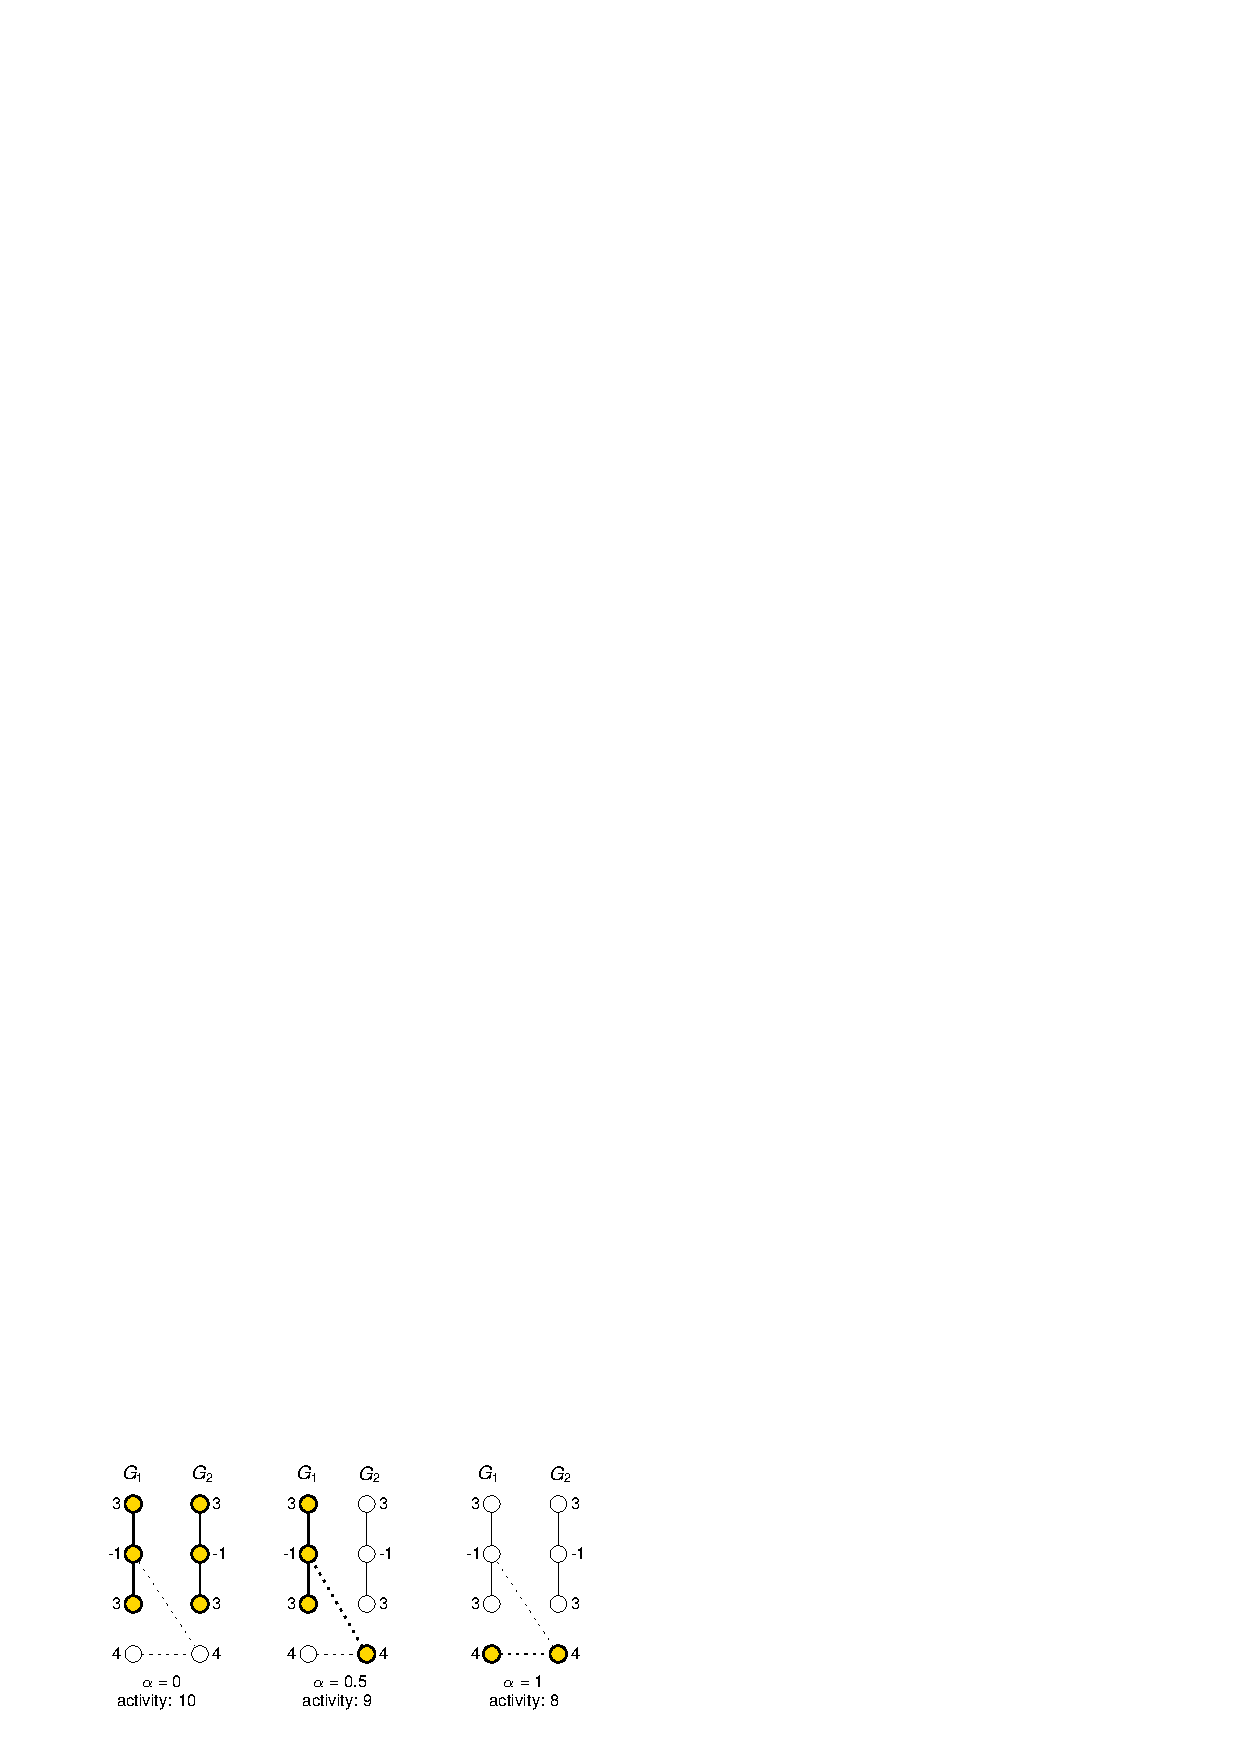
\includegraphics{exmpl_tradeoff_alpha}
			\caption[Trade-off between activity and conservation]{\textbf{Trade-off between activity and conservation.}
				Three optimal solutions (indicated in yellow) for varying conservation ratios $\alpha$ in a toy example instance.
				Node activities are given next to the nodes, conserved node pairs are linked by dotted lines.
				The activity of a conserved module is the sum of the activities of its comprising nodes.
				The parameter $\alpha$ denotes the minimum fraction of nodes in a solution that must be conserved, \ie{} connected by a dotted line.
			}
			\label{fig:exmpl_tradeoff_alpha}
		\end{figure}

	\subsection{Mixed-Integer Linear programming approach}

		We formulate the conserved active modules problem as an integer programming (IP) problem in the following way.
		\allowdisplaybreaks
		\begin{alignat}{3}
		\label{eq:obj}           \max\: & \sum_{v \in V_1 \cup V_2} w_v x_v \\
		\label{eq:m_u}  \text{s.t.}\:\: & m_u = \max_{uv \in R}{x_u x_v} & u \in V_1\\
		\label{eq:m_v}                  & m_v = \max_{vu \in R}{x_u x_v} & v \in V_2\\
		\label{eq:b}                    & \sum_{v \in V_1 \cup V_2} m_v \geq \alpha \sum_{v \in V_1 \cup V_2} x_v &\\
		\label{eq:con}                  & \text{$G_1[\mathbf{x}]$ and $G_2[\mathbf{x}]$ are connected}&\\
		\label{eq:vars}                 & x_v, m_v \in \{0, 1\} & v \in V_1 \cup V_2
		\end{alignat}


		This formulation satisfies the properties of activity, conservation and modularity.

		\paragraph{Activity.}\mbox{}\\
		Variables $\mathbf{x} \in \{0, 1\}^{V_1 \cup V_2}$ encode the presence of nodes in the solution, \ie, for all $v \in V_1 \cup V_2$ we want $x_v = 1$ if $v \in V^*$ and $x_v = 0$ otherwise.
		%\[
		%	x_v = \begin{cases}1 & \text{if } v \in V^*\text{,}\\
		%	                   0 & \text{otherwise.}\end{cases}
		%\]
		The objective function \eqref{eq:obj} uses these variables to express the activity of the solution, which we aim to maximize.

		\paragraph{Conservation.}\mbox{}\\
		Variables $\mathbf{m} \in \{0, 1\}^{V_1 \cup V_2}$ encode the presence of conserved nodes in the solution.
		Recall that a node $u \in V_1^*$ ($u \in V_2^*$) that is present in the solution is conserved if there is another node $v \in V_2^*$ ($v \in V_1^*$) in the solution such that the two nodes form a conserved node pair $uv \in R$ ($vu \in R$).
		This corresponds to constraints \eqref{eq:m_u} and \eqref{eq:m_v}.
		Indeed, constraints \eqref{eq:m_u} encode that a node $u \in V_1$ that is present in the solution ($x_u = 1$) is conserved if there exists a related node $v \in V_2$ ($uv \in R$) that is also present in the solution ($x_v = 1$).
		Similarly, constraints \eqref{eq:m_v} defines conserved nodes in $V_2$ that are present in the solution.
		We linearize $x_ux_v$, in a standard way, by introducing binary variables $\mathbf{z} \in \{0,1\}^R$ such that $z_{uv} = x_ux_v$ for all $uv \in R$:
		\allowdisplaybreaks
		\begin{alignat}{3}
		\label{eq:z1} & z_{uv} \leq x_u                 & uv \in R\\
		\label{eq:z2} & z_{uv} \leq x_v                 & uv \in R\\
		\label{eq:z3} & z_{uv} \geq x_u + x_v - 1 \quad & uv \in R\\
		\label{eq:vars2} & z_{uv} \in \{0,1\} & uv \in R
		\end{alignat}

		Subsequently, we model the max function in \eqref{eq:m_u} and \eqref{eq:m_v} as follows.
		\allowdisplaybreaks
		\begin{alignat}{3}
		\label{eq:m1}   & m_u \geq z_{uv}   & \forall v \in {V_2}^*\text{ st. }uv \in R\\
		\label{eq:m1b}  & m_v \geq z_{uv}   & \forall u \in {V_1}^*\text{ st. }uv \in R\\
		\label{eq:m2}   & m_u \leq \sum_{uv \in R}z_{uv}\quad  & u \in V_1\\
		\label{eq:m3}   & m_v \leq \sum_{uv \in R}z_{uv}  & v \in V_2
		\end{alignat}
		This set of constraints encode the two required conditions:
			\[
				m_u = \begin{cases}1 & \text{if at least one of its counterpart is present,}\\
				                   0 & \text{otherwise.}\end{cases}
			\]
		On one hand, \eqref{eq:m1} define a set of constraints: one for each node $v \in {V_2}^*$ such that $uv\in R$. This set of constraints effectively instruct the ILP that $m_u$ must be 1 if at least one of the counterparts of $u$ is in the solution.
		The same reasoning goes for \eqref{eq:m1b}.
		On the other hand, \eqref{eq:m2} constraint the variable $m_u$ to be 0 if none of the counterparts of $u$ are in the solution.
		The same reasoning goes for \eqref{eq:m3}.

		We model the required degree of conservation by constraint \eqref{eq:b}: the fraction of conserved nodes in the solution is at least $\alpha$.

		\paragraph{Modularity.}\mbox{}\\
		In addition, we satisfy the modularity property by requiring in \eqref{eq:con} that $G_1[\mathbf{x}]$ and $G_2[\mathbf{x}]$ are connected.

		Constraint \eqref{eq:con} states that the nodes encoded in the solution $\mathbf{x}$ induce a connected subgraph in both $G_1$ and $G_2$.
		There are many ways to model connectivity, \eg, using flows or cuts
		\parencite{magnanti1995optimal}.
		However, \textcite{dilkina2010solving} showed that cut-based formulations perform better in practice.
		Recently, \textcite{alvarez2013maximum} have introduced a cut-based formulation that only uses node variables.
		In an empirical study, the authors show that their formulation outperforms other cut-based formulations.
		We model connectivity along the same lines.
		Since the constraints that we will describe are similar for both graphs, we introduce them only for graph $G_1 = (V_1, E_1)$.
		\allowdisplaybreaks
		\begin{alignat}{3}
		\label{eq:sumy} & \sum_{v \in V_1} y_v \leq 1 & \\
		\label{eq:y}    & y_v \leq x_v & v \in V_1\\
		\label{eq:cut}  & x_v \leq \sum_{u \in \delta(S)} x_u + \sum_{u \in S} y_u
                  		\quad & v \in V_1, \{v\} \subseteq S \subseteq{V_1}\\
		\label{eq:vars3} & y_v \in \{0,1\} & v \in V_1 \cup V_2
		\end{alignat}
		Where $\delta(S) = \{ v \in V_1 \setminus S \mid \exists u \in S: uv \in E_1 \}$ denotes the \emph{neighbors} of $S$.

		The modularity property states that $\mathbf{x}$ should induce a connected subgraph in $G_1$.
		However in our model, we don't explicitely model graph connectevity, and model local connectivity instead.
		The first sum of \eqref{eq:cut} state that $x_v$ can only be $1$ if, for all sets $S \subseteq V$ containing $v$, it holds that there is a neighbor $u$ of $S$ in the solution.
		Informally, this constraint is a form of expension where we require the nodes in the solution to be part of the neighborhoud of the other nodes in the solution, hence forming a connected subgraph.
		However this is not sufficient, because this would require all nodes to be included in the end.
		We solve this by introducing binary variables $\mathbf{y} \in \{0, 1\}^{V_1}$ that determine a root node, which serves as a local expension termination condition.
		First, constraints \eqref{eq:sumy} and \eqref{eq:y} state that at most one node $v$ part of the solution can also be the root node -- in which case $y_v = 1$.
		Second, the last sum of \eqref{eq:cut} state that $x_v$ can only be $1$ if, for all sets $S
		\subseteq V$ containing $v$, it holds that the root node is in $S$.
		Informally and integrating the first sum, this constraint encode that the graph is locally connected around $v$ if, for all possible sets $S \subseteq V$ containing $v$, either the root node is part of $S$ or at least one node of the neighborhoud of $S$ is part of the solution.

		There is an exponential number of such constraints.
		Therefore, we cannot add all them to our initial formulation.
		Instead we use a branch-and-cut approach, that is, at every node of the branch-and-bound tree we identify all violated constraints and add them to the formulation.
		Finding violated inequalities corresponds to solving a minimum cut problem, which we do using the algorithm by \textcite{boykov2004experimental}.

		%In the separation, we also generate back cuts and nested cuts.
		%Details are omitted due to space limitation.

		\paragraph{}
		To further improve the performance, we also strengthen our model with the following constraints. None of those constraints are necessary, but they help the ILP solver by reducing the search space.
		\begin{alignat}{3}
		\label{eq:y2}   & y_v = 0 & v \in V, w_v < 0\\
		\label{eq:sumy2} & \sum_{u \in V} y_u \geq x_v & v \in V, w_v\geq 0\\
		\label{eq:1neighbor} & x_v \leq \sum_{u \in \delta(\{v\})} x_u + y_v \quad & v \in V\\
		\label{eq:sym_break} & y_v \leq 1 - x_u \quad & u, v \in V, u < v, w_u \geq 0, w_v \geq 0
		\end{alignat}
		Constraints \eqref{eq:y2} states that the root node must be a positively weighted node, which reduces the search space of the root node.
		Constraints \eqref{eq:sumy2} explicitly state that the root node variable must be 1 if at lease one of the positive nodes is in the solution.
		This was already required for the previous set of constraints but never explicitly instructed to the solver.
		Constraints \eqref{eq:1neighbor} is an optimization for the cases where the set $S$ in \eqref{eq:cut} is a singleton.
		Finally, constraints \eqref{eq:sym_break} are symmetry breaking constraints: they encore an ordering for the possible root selections.
		It effectively requires that among all positively weighted nodes in the solution, the root node is the smallest one -- according to some arbitrary order\footnote{In our case: the order of apperances of the nodes in the network definition.}.
		This last set of constraints also provide determinism: the ordering garantee that two runs of the ILP will choose the same root node.

\section{Material and methods}
\label{sec:xexp}

We apply our method to the recently discovered interleukin-17 producing helper T~cells (Th17), which exposes the problems highlighted in \cref{sec:xhintro}.

These cells form a separate subset of helper T~cells with a differentiation pathway distinct from those of the established Th1 and Th2 cells \parencite{park2005distinct}.
Th17 cells are known to contribute to pathogenesis of inflammatory and autoimmune diseases such as
asthma, rheumatoid arthritis, psoriasis and multiple sclerosis and play also a role in cancer immunology \parencite{wilke2011deciphering}.
They originate from na\"ive helper cells, responding to environmental stimulus by activating a differentiation and specialization process \parencite{steinman2007brief}.

Understanding the pathways and regulatory mechanisms that mediate the decision making processes resulting in the formation of Th17 is a critical step in the development of novel therapeutics that will facilitate rational manipulation of the immune response.
Unfortunately, the vast majority of data collected so far originates from studies performed on mice \parencite{tuomela2012identification} and, most importantly, a comprehensive comparison of the Th17 differentiation process in model organisms and in human is missing.
Several studies indicate that the differentiation and phenotype of human and mouse Th17 cells are similar \parencite{annunziato2009studies}.
Both subsets serve similar pro-inflammatory functions and produce the same hallmark cytokines and similar receptors.
Furthermore, most of the already identified regulator genes show high sequence conservation.

These findings indicate that the differentiation process seems well conserved between human and mouse and that a cross-species approach is reasonable.
Other studies, however, show stimulus requirements for effective differentiation of human cells that differ from those required for mice \parencites{mcgeachy2008th17}{o2008differentiation}{annunziato2009human}.

The simultaneous analysis of both human and mouse expression data allows the identification of conserved candidate regulators% that are likely to be key regulators of the differentiation process
, as well as potential drug targets.
Most of our current understanding on Th17 cell differentiation relies on studies carried out in mice, whereas the molecular mechanisms controlling human Th17 cell differentiation are less well defined.
A characterization of the similarities and differences will not only increase our understanding of this fundamental process, but is also essential for sound translational research.

	\subsection{Experimental procedure}

% In \citet{Tuomela:2013ly}, RNA-Seq samples of both human and mouse CD4+ cells
	% were polarized toward Th17 direction and we summarize here their
	% experimental procedure. Human CD4+ cells were obtained from  mononuclear
	% cells purified from the umbilical cord blood of healthy neonates. Cells
	% from several individuals were pooled, then activated using anti-CD3 and
	% anti-CD28. Th17 differentiating cytokines consisted of IL6, IL1B and TGFB,
	% along with neutralizing anti-IFNG and anti-IL4. Cells that were activated
	% without Th17 cytokines were cultured as controls (Th0). Mouse CD4+ cells
	% were obtained from C57BL/6 mice bred under specific conditions devoid of
	% pathogens. Similarly to human cells, mouse CD4+ cells were activated
	% (anti-CD3 and anti-CD28), polarized (TGFB, IL6, IL1B) and control mouse
	% cells (Th0) were also cultured. Three biological replicates of mouse and
	% human cells, for both conditions, were collected at \unit{0}5]{h},
	% \unit{1}{h}, \unit{2}{h}, \unit{4}{h}, \unit{6}{h}, \unit{12}{h},
	% \unit{24}{h}, \unit{48}{h}, \unit{72}{h} time points. Following
	% manufacturer instructions, RNA was isolated and DNase treated before being
	% sequenced (50nt reads) on a HiSeq \comment[Daniela]{Do we know the HiSeq
	% version? 1000, 2000, 2500?} instrument. Base calling and quality control
	% was performed using CASAVA 1.8.

We summarize here the experimental procedure followed by \textcite{tuomela2012identification} and \textcite{yosef2013dynamic} to generate transcriptomic profiles.

\textcite{tuomela2012identification} isolated CD4+ T-cells from umbilical cord blood of several healthy neonates, arranged in three different pools, then activated with anti-CD3 and anti-CD28.
Cells from each pool were then divided in two batches, one to be polarized toward Th17 direction, and one serving as control (Th0).
Th17 differentiating cytokines consisted of IL6~(\unit{20}{\nano\gram\per\milli\liter}), IL1B~(\unit{10}{\nano\gram\per\milli\liter}) and TGFB~(\unit{10}{\nano\gram\per\milli\liter}), along with neutralizing anti-IFNG~(\unit{1}{\micro\gram\per\milli\liter}) and anti-IL4~(\unit{1}{\micro\gram\per\milli\liter}).
%Cells that were activated without Th17 cytokines were cultured as controls (Th0).
Three biological replicates of human cells, for both conditions (coming from each pool), were collected between \unit{0.5-72}{h} (\unit{0.5}{h}, \unit{1}{h}, \unit{2}{h}, \unit{4}{h}, \unit{6}{h}, \unit{12}{h}, \unit{24}{h}, \unit{48}{h}, \unit{72}{h} time points) and hybridized on Illumina Sentrix HumanHT-12 Expression BeadChip Version~3.
The microarray data were analyzed using the beadarray Bioconductor package \parencite{dunning2007beadarray}.

\textcite{yosef2013dynamic} purified CD4+ T-cells from spleen and lymph nodes from wild type C57BL/6 mice, then activated with anti-CD3 and anti-CD28. For Th17 differentiation, cells were cultured with TGFB (\unit{2}{\nano\gram\per\milli\liter}), IL6 (\unit{20}{\nano\gram\per\milli\liter}), IL23 (\unit{20}{\nano\gram\per\milli\liter}) and IL1B (\unit{20}{\nano\gram\per\milli\liter}) during \unit{0.5-72}{h} (at time points \unit{0.5}{h}, \unit{1}{h}, \unit{2}{h}, \unit{4}{h}, \unit{6}{h}, \unit{8}{h}, \unit{10}{h}, \unit{12}{h}, \unit{16}{h}, \unit{20}{h}, \unit{24}{h}, \unit{30}{h}, \unit{42}{h}, \unit{48}{h}, \unit{50}{h}, \unit{52}{h}, \unit{60}{h}, \unit{72}{h}), and finally hybridized on an Affymetrix HT\_MG-430A.
%Highly-correlated replicates were generated for 8 time points (\unit{1}{h}, \unit{4}{h}, \unit{10}{h}, \unit{20}{h}, \unit{30}{h}, \unit{42}{h}, \unit{52}{h}, \unit{60}{h}).


\subsection{Microarray processing, statistical analysis and node scoring}
\label{sub:statistical_analysis_and_node_scoring}
% Sequence reads were mapped using TopHat 1.3.2 to the GRCh37 release 63 human
% genome and to the NCBIM37 release 63 mouse genome. Gene-wide read counts for
% Ensembl genes were estimated using HTSeq 0.5.4p5, discarding reads overlapping
% multiple genes. Differential expression between Th17 and Th0 conditions was
% estimated using the edgeR package \citep{Robinson:2010ve}.

% For each species, differential expression calling was performed at each time point independently.
% For the human samples, samples were indicated as paired according to the
% experimental design so as to account for the pooled human samples. For mouse
% samples, calling was performed on all Th0 vs Th17 samples, regardless of the
% mouse donor. In both cases, dispersion was estimated as gene-wise dispersion.


Preprocessed and quantile normalized data sets were downloaded from GEO under the accession numbers GSE43955 and GSE35103.
As downloaded from GEO, both the human and the mouse time-series were already filtered by retaining only the probes with detection p-values $< 0.05$ in at least one time point and one condition.
Following the original studies, we further only retained probes having a standard deviation $> 0.15$ over all the conditions and time points; as well as being annotated by a single Ensembl gene.
Finally, a single probe was selected for each gene by taking, for each Ensembl gene, the probe having the largest variance accross all samples.
In total, 12,307 and 18,497 probes passed the filters for the mouse and human data set, respectively.

Differential expression between Th17 and Th0 conditions were estimated using the limma package \parencite{smyth2005limma}.
Human samples were indicated as paired according to the experimental design so as to account for the pooled human samples.
For mouse samples, calling was performed on all Th0 vs Th17 samples, regardless of the mouse donor.
To determine which genes were differentially expressed at a given time point, we used a linear model to estimate the interaction between the treatment and the time effect.
The linear models used for the human and mouse studies include one interaction term for each time point and exclude the intercept (In R, the formula reads: $\mathrm{\sim 0+treat:time}$).
% \textcolor{red}{The linear models used in each of the human and mouse studies are defined as $\mathrm{\sim 0+treat:time}$, interpreted as 1) no intercept term and 2) one interaction term for each time point (R formula syntax).
Differential expression at any time point $K$ of interest were determined by the contrasts $\mathrm{Th17.time_{K} - Th0.time_{K}}$.
We report in this study results for the following time points: \unit{2}{h}, \unit{4}{h}, \unit{24}{h}, \unit{48}{h}, \unit{72}{h}.

%To deal with the lack of replicates in the highly variable late time points of
%the mouse data (\unit{2}{h}, \unit{24}{h}, \unit{48}{h}, \unit{72}{h}), we
%relied on the neighboring time point to estimate the
%treatment effect in this time frame by performing a weighted regression. For
%example, identification of differential expression at \unit{48}{h} is made by
%estimating the effect $8/10 \cdot Th17 : time_{48} + 1/20 \cdot Th17 : time_{42}
%+ 3/20 \cdot Th17:time_{50}$.


%%%% Old probe selection procedure 
% Once differential expression was tested for at the probe-level, we
% summarized the results at the gene-level by taking the smallest
% p-value of any probe capturing a transcript of that gene. 
\noindent\paragraph{}\noindent Following \parencite{dittrich2008identifying}, we computed positive and negative scores for each gene at each time point by fitting a beta-uniform mixture model using the implementation in the BioNet package \parencite{beisser2010bionet}.
The method proceeds as follows:

Similarly to \parencite{pounds2003estimating}, the distribution of the gene-wise p-values $x = x_1, \ldots, x_n$ is described as a beta-uniform mixture (BUM) model, which is a mixture of a $B(a, 1)$ beta distribution (signal) and a uniform distribution (noise):   % By definition the
% p-value is uniformly distributed under the null hypothesis
% (noise).
% the combined
% distribution of signal and noise p-values can empirically be modelled
% by a beta-uniform mixture (BUM) model, where the signal component is modeled by a beta distribution $\Beta(a,1)$ and the noise component is modeled by a uniform distribution:
% The $\Beta(a,b)$ distribution is given by
% \begin{eqnarray*}
%    f(x) & = & \frac{\Gamma(a+b)}{\Gamma(a)\Gamma(b)}\;x^{a-1}(1-x)^{b-1},
% \end{eqnarray*}
% where $\Gamma(\cdot)$ denotes the Gamma function.
% The distribution of the derived p-values reduces to
$\lambda + (1- \lambda)ax^{a-1}$, for $0 < a < 1$, with mixture parameter  $\lambda$ and shape parameter $a$ of the beta distribution.
The log likelihood is defined as $\log\left(\lambda, a;x\right) = \sum_{i=1}^{n}\log(\lambda+(1-\lambda)a x_i^{a-1})$, and consequently the maximum-likelihood estimations of the unknown parameters are given by $[\hat{\lambda}, \hat{a}] = \argmax_{\lambda,a} \left(\lambda,a;x\right)$.
%%\begin{equation*}
%   . %%\enspace.
%%\end{equation*}
The parameter estimates have been obtained using numerical
optimization. % Based on the fitted mixture model the distribution of
% p-values can be decomposed into a signal and a noise component, from
% which the node score is calculated as a log likelihood ratio of the signal and the noise component.
% Similar to classical hypothesis tests, a threshold value that
% discriminates signal from noise can be introduced.
As detailed in \parencite{pounds2003estimating}, the BUM model allows the estimation of a false discovery rate ($\FDR$) that can be controlled via a p-value threshold $\tau(\FDR)$.
The adjusted log likelihood ratio score is then defined as
\[
% \begin{eqnarray}
%    S^{\FDR}(x)  = \log\left(\frac{\Beta(a,1)(x)}{\Beta(\tau^{\FDR},1)(x)\Beta(1,1)(x)}\right) =   \log\left(\frac{a x^{a-1}}{a \tau^{a-1}}\right) = (a-1)\left(\log(x) - \log(\tau(\FDR))\right),
s(x, \FDR) =   \log\frac{\hat{a} x^{\hat{a}-1}}{\hat{a} \tau(\FDR)^{\hat{a}-1}}
= (\hat{a}-1)\left(\log(x) - \log(\tau(\FDR))\right)\:.
\label{eqn:scoreFDR}
\]
%The adjusted and unadjusted scores only differ by an additive offset
%which is dependent on the parameter $\tau_{\FDR}$ and can be regarded
%as a significance threshold. Thus, 

Genes whose differential expression is considered significant given the FDR threshold obtain a positive score while genes showing no differential expression will receive a negative score. % It can easily be seen that for $\tau(\FDR) \rightarrow 0 $ the score $s(x) \rightarrow -\infty$ and for $\tau(\FDR) \rightarrow 1$ all scores will be positive and the $\FDR$ will be equal to $\lambda$, the mixture parameter of the noise model.
The size of the resulting module can be regulated with this FDR parameter.
Throughout this study, $\FDR=0.1$ was used for all samples and species.

However, due to the experimental noise and paired design, the human samples have much higher intra-group variance, resulting in significant calls having p-values orders of magnitude higher than the mouse calls.
This results in a range of scores that is much narrower for human than for mouse, possibly imbalancing results towards mouse modules.
To correct for this effect, scores of mouse genes were rank normalized to the scores of the human genes as follows: the scores (as defined by the BUM model) were sorted, and for each gene the score of the $i$-th mouse gene was set to the score of the $i$-th human gene.

Comparison of the distribution of scores before and after normalization showed that compared to usual Benjamini-Hochberg FDR and log fold change cut-offs ($\absLOGFC \geq 1)$, the loss in statistical power was inconsequential and that this procedure ensured that mouse and human genes had comparable score distributions.

% In the following, all reported FDRs were obtained using the Benjamini-Hochberg procedure.
%Finally, only genes coding for a protein present in the STRING network (see Sect.~\ref{sub:public_datasets}) were kept. % Table \ref{table:calls} summarizes the number of differentially expressed genes called at each time point for the two species.


% \begin{table*}[ht]
% \label{table:calls}
% \centering
% \begin{tabular}{r|l|ll || lrrrrr}
% \multirow{2}{*}{Species} & \multicolumn{3}{c||}{Gene characteristic} &  \multicolumn{5}{c}{Time} \\
% \cline{2-9}
%  ~ & BUM score & $FDR\leq 0.01$ & $abs(LogFC) \geq 1.0$ & 2h & 4h & 24h & 48h & 72h \\
% \hline
% \hline
% %  \cline{2-9}
%  \multirow{6}{*}{Human} & \multirow{2}{*}{Negative} & False & False & 8355 & 8424 & 8346 & 8282 & 8189 \\
%   ~ & ~ & False & True &  17 &  23 &  26 &  22 &  19 \\
%   \cline{2-9}
%   ~ & \multirow{4}{*}{Positive} & False & False &   4 & 0 &   4 &  10 &  65 \\
%   ~ & ~ & False & True &   2 & 0 & 0 &   1 &   2 \\
%   \cline{3-9}
%   ~ & ~ & True & False &  37 &   2 &  39 &  75 & 99 \\
%   ~ & ~ & True & True &  38 &   4 &  38 &  63 &  79 \\
%   \hline
%   \hline
%   \multirow{6}{*}{Mouse} & \multirow{4}{*}{Negative} & False & False & 6569 & 6655 & 6422 & 6146 & 5542 \\
%   ~ & ~ & False & True &  59 &  17 & 73 &  25 & 38 \\
%   \cline{3-9}
%   ~ & ~ & True & False & 115 & 108 & 106 & 405 & 790 \\
%   ~ & ~ & True & True & 98 &  65 & 163 & 204 & 343 \\
%   \cline{2-9}
%   ~ & \multirow{2}{*}{Positive} & True & False & 11 &   1 & 2 &   5 & 4 \\
%   ~ & ~ & True & True &  52 &   7 &  62 & 124 & 201 \\
%    \hline
% \end{tabular}
% \caption{Contingency table summarizing the characteristics of the nodes used as input to \xHeinz for the identification of conserved Human and Mouse modules during Th17 differentiation. In this setup, \xHeinz received as input two species-specific STRING network, a mapping between Human and Mouse proteins based on ENSEMBL orthology, and a mapping from protein to a real-valued Beta-Uniform (BUM) score. Each cell in this table reports the number of genes coding for a protein from the species-specific STRING network, for each of the 5 instances (2h--72h), for each species, and satisfying any conjunction of these three properties: 1)~\textbf{BUM score:}~being scored positively using a rank-normalized BUM decomposition of the distribution of the p-values of differential expression between Th17 and Th0 conditions (limma moderated t-test); 2)~\textbf{FDR:}~having a Benjamini-Hochberg FDR below $\tau\leq0.01$ under the same hypothesis and 3)~\textbf{logFC:}~having an absolute log-fold change $\geq 1$. Rows containing only zeros are omitted. Details are provided in section \ref{sub:statistical_analysis_and_node_scoring}.}
% \end{table*}
% \comment{Consider increasing the logFC threshold to 1.5 or 2}

\subsection{Network and orthology databases}
\label{sub:public_datasets}

The human and mouse background networks were downloaded from STRING v9.1, protein.actions.detailed.v9.1.txt \parencite{franceschini2013string}, which is a database that contains experimentally verified direct protein interactions.
Note that this network also contains interactions predicted based on orthology, so-called \emph{interologs}.
Ideally, we would prefer to use only experimentally predicted interactions, but currently, for mouse, such available data is too incomplete to result in a meaningful background network.
Outlier nodes with a degree above $40$ times the interquartile range plus the 75th percentile of the distribution of all node degrees were removed (ELAVL1, UBC, Ubb, Ubc).
The resulting mouse network has $16,821$ nodes and $483,532$ edges and the human network has $16,255$ nodes and $315,442$ edges.


For any given timepoint, we performed a preprocessing step where we retained the subgraphs of the input networks induced by the genes that meet the microarray filtering criteria.
This reduced the number of nodes to 8,453 human nodes, 6,882 mouse nodes and 14,779 nodes in the orthology mapping.
Among these, up to 250 nodes (depending on the time point) have positive scores.
The rank normalization as described in \cref{sub:statistical_analysis_and_node_scoring} ensured that the number of positive human nodes is in the order of the number of positive mouse nodes.

Orthology information was downloaded from Ensembl release 59 \parencite{flicek2013ensembl} and all human and mouse orthologs were kept, regardless of the identity scores.
The orthology mapping corresponds to a bipartite graph involving $67,304$ human proteins and $43,953$ mouse proteins linked by $104,007$ edges, grouped in $16,552$ bicliques with an average size of $6.72$ proteins (SD: $5.34$).

	\subsection{Results}

		\subsubsection{\xheinz{} identifies statistically significant conserved modules at different levels of conservation}
		\label{sec:xheinz-effic-ident}

			We applied \xheinz{} on samples from the Th17 human and mouse data sets for time points \unit{2}{h}, \unit{4}{h}, \unit{24}{h}, \unit{48}{h} and \unit{72}{h}.
			We solved these instances for different values of $\alpha \in [0, 1]$ with a step size of $0.1$.
			All computations were done in single-thread mode on a desktop computer (Intel XEON e5 3~Ghz) with 16~Gb of RAM and a time limit of 12,000 CPU seconds.
			After this timeout, the best feasible solution is returned by the solver.

			\Cref{fig:scores} shows for the five time points and eleven values of the $\alpha$ parameter, the human and mouse scores of the found modules as well as the distribution of the module contents.
			For 26 of the 55 instances we solved the conserved active modules problem to provable optimality  within the time and memory limit.
			The optimality gap of a solution is defined as $(\mathit{UB} - \mathit{LB}) / \abs{\mathit{LB}}$, where $\mathit{LB}$ and $\mathit{UB}$ are the value of the best solution and the lowest upper bound as identified by the branch-and-cut algorithm, respectively.
			Of the 29 instances that are not solved to optimality, 22 have a gap smaller than $5\%$.

\begin{figure}[btp]
  \centering
  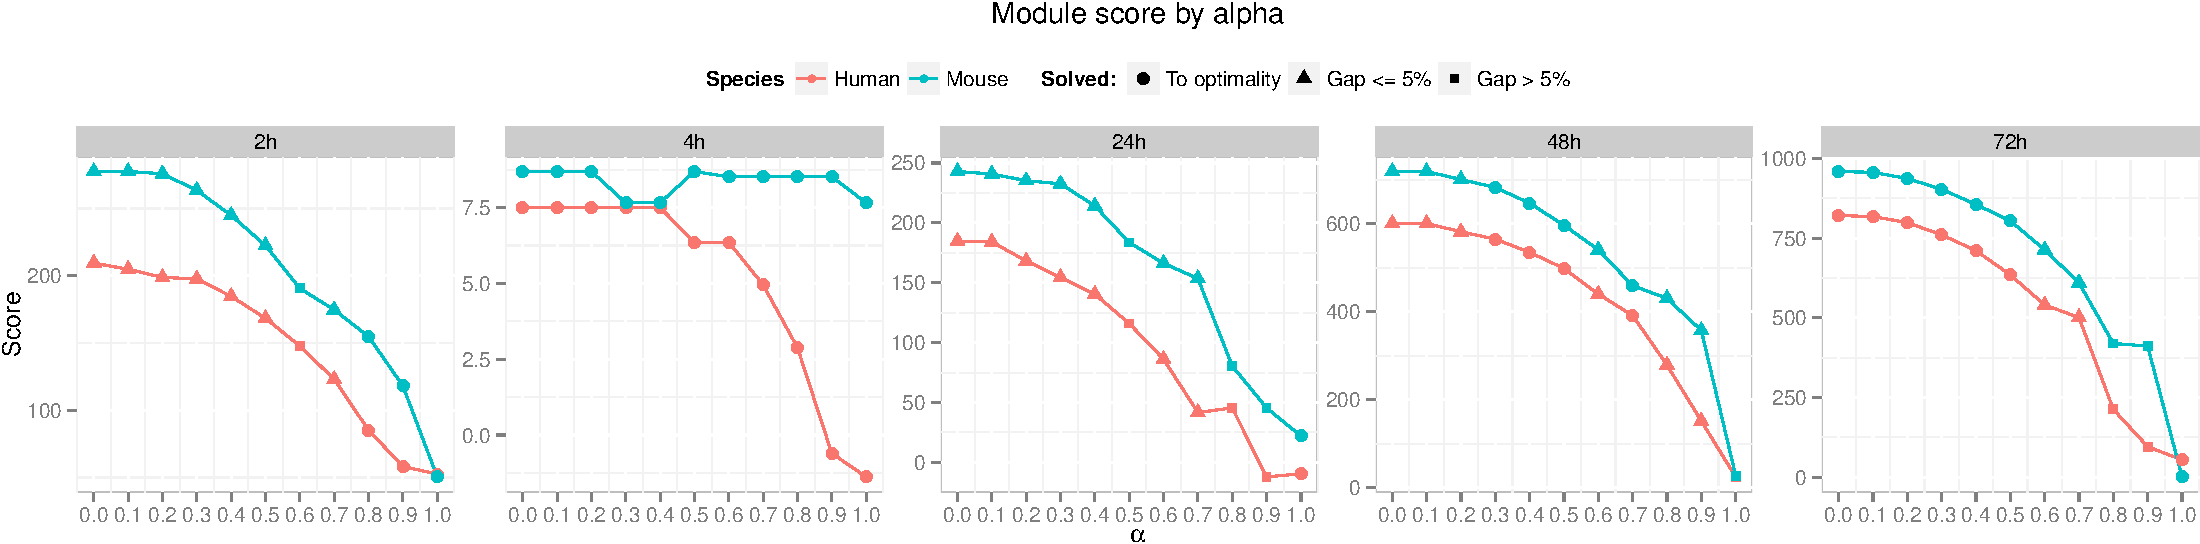
\includegraphics[width=\linewidth,trim=0 0 0 10mm,clip]{img/score_by_alpha_array-crop.pdf}\\
  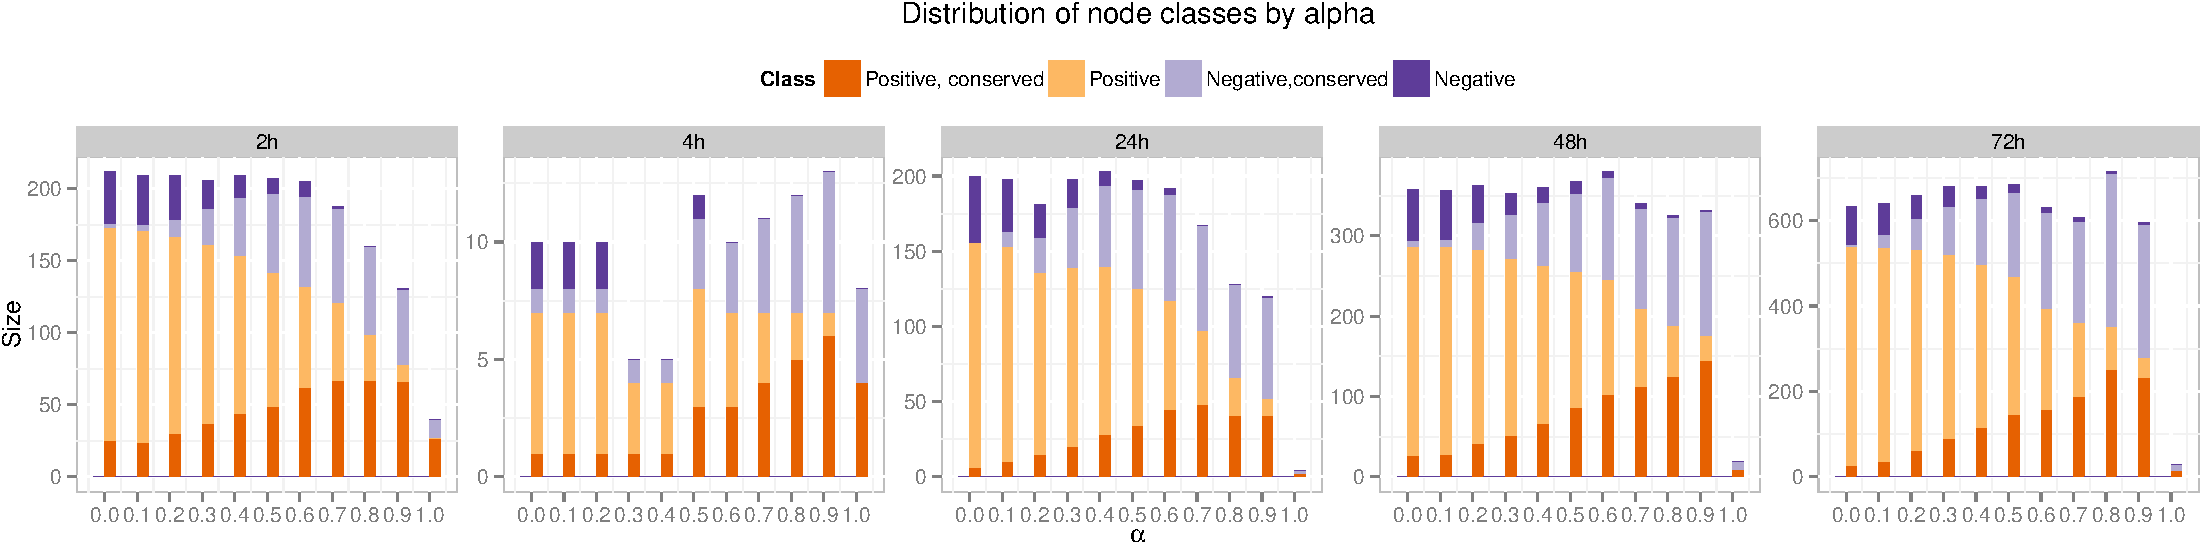
\includegraphics[width=\linewidth,trim=0 0 0 10mm,clip]{img/node_classes_by_alpha_array_scores-crop.pdf}
  \caption[Statistics of \xheinz{} solutions]{\textbf{Statistics of \xheinz{} solutions.}
  	  The conserved active module problem was solved for five time points (columns) over a sequence of 11 consecutive values of the $\alpha$ conservation parameter ($x$-axis).
  	  We report in the top row the score of the best solution ($y$-axis) and whether optimality was proven by our algorithm (circles).
  All runs were limited to 12,000 CPU seconds on a standard desktop computer.
  The second row illustrates how module contents vary as $\alpha$ increases.
  The height of each bar indicates the size of the respective module, colors indicate the fraction of positive and conserved nodes.
  \label{fig:scores}}
\end{figure}

Any feasible solution for a conservation ratio of $\alpha$ is also a solution for any $\alpha' \leq \alpha$.
We indeed see in \cref{fig:scores} that this property holds, the solution values decrease monotonically with increasing $\alpha$.
Consequently, if we obtain an optimal solution (\ie, with maximal activity score) for $\alpha'$ then, any solution for $\alpha$ must have its activity score that is greater or equal to the one for $\alpha'$.
When we only account for the optimal solutions of our instances, we indeed see that this property holds.
% MEK: I DON'T UNDERSTAND THIS THE FOLLOWING
%Conversely, this implies that we can bound the optimal activity scores whenever
%we obtain optimal solutions for neighboring $\alpha$ parameter values; and thus that
%several of our solutions were close to the real optimum. 
% HS: Mohammed, as an example, take 48h 0.5 and 0.8, both are solved to optimality. This imply that the score of the optimal solutions for 0.6 and 0.7 are within the scores of the 0.5 and the 0.8, and since our suboptimal solutions are within this range, this means that we not so far from them. 

As an added validation, we observe that the solutions for $\alpha=0$ (no conservation constraints) are identical to the solutions obtained by running the single species method Heinz, described by \textcite{dittrich2008identifying}, separately on the two networks.

There is a sharp decrease in module size for $\alpha = 1$.
Indeed, this is the most restrictive setting since it enforces that all the nodes in a module must be conserved.
We also observe that as $\alpha$ increases, both positive and negative \emph{conserved} nodes are added, indicating that we manage to retrieve informative nodes in a gradual manner.
See also \cref{app:significance} for a detailed analysis of module overlap for all combinations of $\alpha$ values.

When we compare solutions across time points, we see that the conserved active modules capture two phases of the differentiation process.
We observe high activity at \unit{2}{h} as well as at the late time points.
Several authors reported such biphasic behavior during early Th17 differentiation, for example \textcites{ciofani2012validated}{yosef2013dynamic} in mouse, and \textcite{tuomela2012identification} for human.
The low activity score observed at the \unit{4}{h} time point is in line with \textcite{yosef2013dynamic}'s mouse studies, which suggest that after the initial induction sustained by Stat3 and Stat1 in the first four hours, a phase of Rorc induction takes place and lasts until the \unit{20}{h} time point, after which the effective protein level of Rorc starts to increase and to trigger the cytokine production phase.
Our model and the solutions obtained suggest that these dynamics are conserved between the two organisms.

Furthermore, \cref{fig:spider-xheinz_modules} illustrates the strong conservation of these overall dynamics, in human and mouse at \unit{2}{h}.
The plots show that in our modules all but two conserved gene pairs change expression in the same direction.
It is worth noting that we do not enforce any conservation of directionality in the \xheinz{} model.

\begin{landscape}
\begin{figure}[h]
  \centering
  %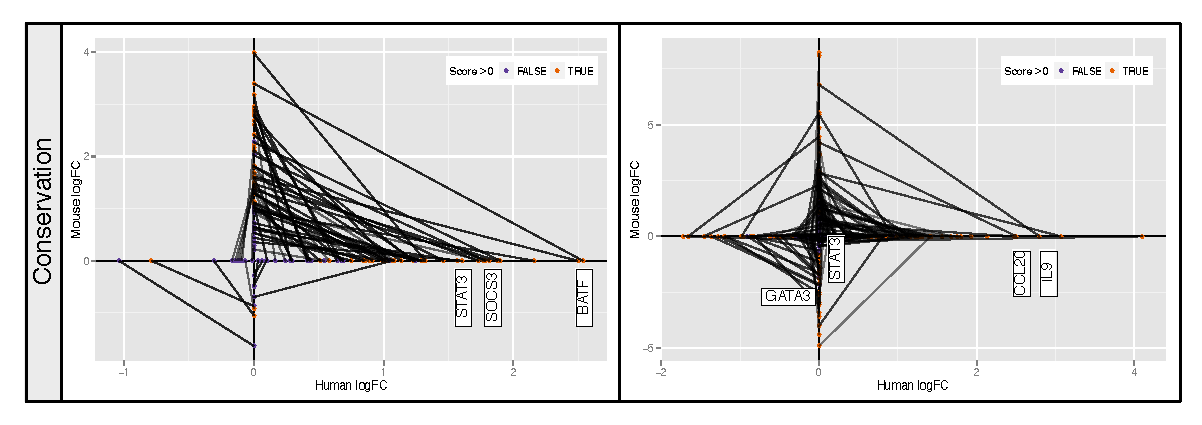
\includegraphics[width=1\linewidth]{spider_panel.pdf}
  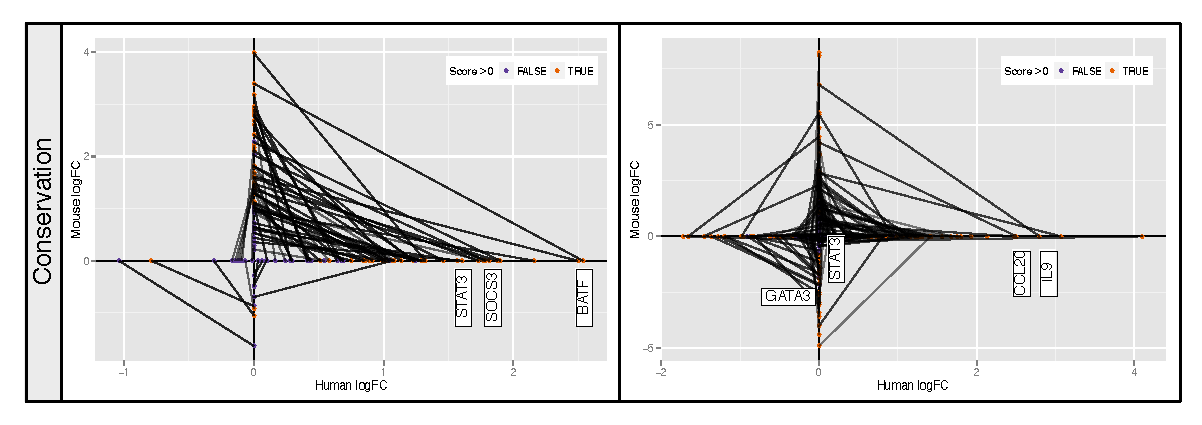
\includegraphics{spider_panel.pdf}
  \caption[Comparison of log fold change expression in mouse and human for conserved gene pairs at \unit{2}{h} and \unit{48}{h}]{\textbf{Comparison of log fold change expression in mouse and human for conserved gene pairs at \unit{2}{h} (left) and \unit{48}{h} (right).}
 Each panel shows the log fold change correlation between conserved gene pairs:
 For each pair, a line segments connects the human logFC ($x$-axis) to the mouse
 logFC ($y$-axis). Point color indicates whether the human or mouse gene has a
 positive score.
      A line segment in the 1st or 3rd quadrant
   signifies positively correlated logFC values whereas a link in the
   2nd and 4th quadrant corresponds to negative correlation. The sign
   of the activity score is indicated by the coloring. Genes discussed
   in the main text are indicated with white boxes.}
  \label{fig:spider-xheinz_modules}
\end{figure}
\end{landscape}


\subsubsection{Early regulation of Th17 differentiation is conserved between human and mouse}
\label{sub:main_regulation_of_th17_differentiation_is_conserved_between_human_and_mouse}

In the following, we study the two phases of the Th17 differentiation process in more detail.
We focus on the \unit{2}{h} and \unit{48}{h} time points.
We selected for this evaluation $\alpha=0.8$ for both time points, as this value provides a balance between conservation and activity and produces modules of interpretable size.
All results at all time points are available on the accompanying website.
\Cref{fig:panel_wht-xheinz_modules} reports a reduced version of the resulting human and mouse Th17 modules for the two time points, and \cref{fig:full_1} and \cref{fig:full_2} show the full, unfiltered module contents of the modules.

We assess statistical significance of the resulting modules by performing 100 runs on randomized networks for each value of $\alpha$, and additional 400 runs for the selected $\alpha=0.8$.
We do this using two randomization methods: (1) permuting the node weights while keeping the graph fixed, and (2) permuting the network topology while keeping the node weights and the node degrees fixed as described in \parencite{mihail2003markov}.
With the exception of a few extreme cases at the \unit{48}{h} time point, all modules were found to be highly significant.
For details see \cref{app:significance}.

Our model for conserved modules relies on the hypothesis that similar biological processes between two related species are realized by orthologous genes.
To evaluate the relevance of the conserved modules returned by \xheinz, we solved the conserved active modules problem between the Th0 and Th17 conditions at \unit{2}{h} and \unit{48}{h}.

At the \unit{2}{h} time point, \xheinz{} identifies a conserved module consisting of $58$ human and $50$ mouse proteins.
Interestingly, both the human and mouse modules are centered around STAT3/Stat3, even if these genes are not the ones showing the higher fold change in both species.
STAT3 is a signal transducer having transcription factor activity and was shown to play a key role in the differentiation process of Th17 \parencite{harris2007cutting}.
Once activated by Th17 polarizing cytokines (such as IL6 in our case), it eventually binds to the promoter regions of IL17A/Il17a and IL17F/Il17f cytokines and activates transcription.
These cytokines are the hallmark cytokines produced by activated Th17 cells.
It is worth noting that IL17/Il17 cytokines and associated receptors are not in the \unit{2}{h} modules, as these proteins have been shown to be expressed only at later time points \parencite{tuomela2012identification}.
Moreover, STAT1/Stat1, another member of the STAT family, is part of the solution and belongs to the central core of the human and mouse modules, which is consistent with its major role during the early phases of Th17 differentiation \parencite{yosef2013dynamic}.


%%Il17a vs IL17F 
%We also observe that the STAT3/BATF/IL6ST/SOCS3 region of the \unit{2}{h} module is well-conserved.
%NOTCH1 has been recently implicated as an intrinsic requirement for Th17 polarization both in human and mouse.
%NOTCH1 directly targets the IL17 and RORC loci and its deficiency is associated with impaired Th17 differentiation~\parencite{keerthivasan2011notch}.
%We further expected that NOTCH1 is implicated in the early phase of the differentiation process as it directly activates transcription of these two Th17 hallmarks proteins that are expressed later.
%Similarly, Batf has been shown to directly control Th17 differentiation in mouse~\parencite{schraml2009ap} and BATF proteins are detected as early as after \unit{12}{h} of polarization in human~\parencite{tuomela2012identification}. 
%Similarly, SOCS3 is a known IL6 and IL21-induced negative regulator of Th17 polarization, that is eventually down-regulated by TGFB and IL6ST at a later phase in order to prolong STAT3 activation \parencites{zhu2008socs3,qin2009tgf}.
%
%Overall, these modules show highly conserved and significant enrichment for response to cytokine stimulus (Benjamini-Hochberg (BH) FDR 5.6e-4), JAK-STAT (BH FDR 4.8e-4) cascade and transcription regulator activity (BH FDR 2.3e-4), computed using the DAVID functional annotation chart \parencite{huang2008systematic}.
%This indicates that the identified module matches expected biological mechanisms observed at early phases~\parencite{ciofani2012validated}.
%Furthermore, comparison of the dynamics of expression shows that genes differentially expressed in both species change expression in the same direction (see Supplementary~Text~A.3).

%\comment[Hayssam]{Add IL2RB/CXCR5 details? Add SOCS3 role. STAT1, easily
%involved. STAT1 implicated in the early phase, STAT3 in all phases [ciofiani]}

We also applied \xheinz{} to find a conserved module at a later time point (\unit{48}{h}).
Kinetics analysis of Th17 differentiation showed that the effective secretion of Th17 hallmark cytokines only happens after several days of polarization \parencites{tuomela2012identification,yosef2013dynamic} and we do observe in these modules a significant enrichment for interleukin related proteins present in both species, which was absent for the \unit{2}{h} modules, such as up-regulation of IL9/Il9.
Secretion of IL9 by Th17 cells have been demonstrated both in mouse and human cells \parencite{beriou2010tgf}, Il9 is known to be induced by Bcl3 \parencite{richard1999interleukin}, and Bcl3 inhibition has been recently shown to affect the function of Th17 cells in mouse \parencite{ruan2010roles}.
We also observe the conserved down-regulation of GATA3/Gata3, which is known to be the master regulator of Th2 cells \parencite{zheng1997transcription}, and is likely to constrain the Th17 regulation program \parencite{van2008enforced}.
Similarly to the modules found at \unit{2}{h}, the \unit{48}{h} modules are centered around STAT3, although at the \unit{48}{h} time point this gene is not differentially expressed anymore neither in human or mouse (resp.\ logFC of 0.17, score of -4.59 for human, and logFC 0.52, score of -3.21 for mouse).
This observation is in line with the major role of STAT3 along the differentiation process at all time points \parencite{yosef2013dynamic}.
To the contrary, STAT1 has been indicated as an exclusively early regulator \parencite{yosef2013dynamic} in mouse and is indeed not present anymore in the \unit{48}{h} modules.%, even though Stat1 is called as differentially expressed in the mouse measurements (BH FDR of $2e-04$, score of $-3.16$ for mouse; BH FDR of $0.99$, score of $-6.54$ for human).
%This demonstrates the strength of performing module identification in both species simultaneously in our setup.
%\comment[Hayssam]{Find ref about plasticity in the early tp. Compute overlap between early and late?}
% , the lack of evidence for differential expression in mouse (FDR 0.93) as well as the conservation constraint in the \xheinz formulation 

We also observe the presence of the RORA/RORC/Rora/Rorc members of the RORs family of intracellular transcription factors, which are considered to be the master regulators of the Th17 lineage \parencite{yang2008t}, and have been implicated in both species \parencite{crome2009role}.
Interestingly, these regulators are linked to the up-regulation of the vitamin-D receptor (VDR/Vdr), whose role in Th17 differentiation and several human auto-immune related disease have been recently studied \parencite{chang2010vitamin}.

\paragraph{}
In summary, our findings show the relevance of the identified conserved active modules with regard to the biological process of interest.
By requiring the active modules to contain a certain fraction of conserved nodes, \xheinz{} identifies the main core proteins involved in the differentiation of Th17.
Our analysis confirms that these proteins are very likely to have similar roles in both species.

\begin{figure}[t]
  \centering
  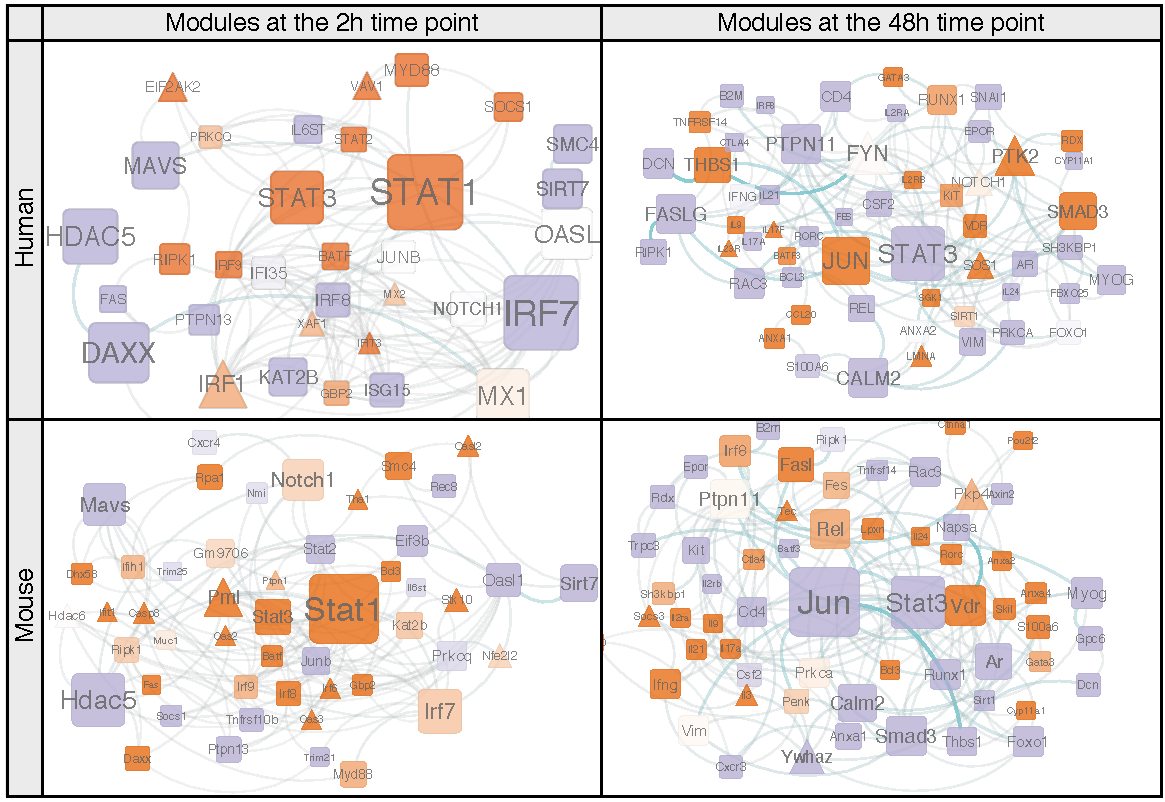
\includegraphics[width=\linewidth]{img/modules_panel.pdf}
  \caption[Conserved active Th17 differentiation modules in human and mouse at \unit{2}{h} and \unit{48}{h}]{\textbf{Conserved active Th17 differentiation modules in human and mouse at \unit{2}{h} and \unit{48}{h}.}
  We obtained node activity scores capturing the significance of differential gene expression between the Th17 and Th0 conditions in human and mouse using the BUM model with $\FDR = 0.1$.
  \xheinz{} uses these scores to search for conserved active modules in the STRING protein action network.
  The first row shows the human counterparts of the best scoring conserved modules for the \unit{2}{h} (left) and \unit{48}{h} (right) samples.
  The second row depicts the mouse counterparts.
  Rounded squares depict genes for which a homolog -- as defined by Ensembl -- is present in the counterpart, whereas triangles denote non-conserved genes.
  Node color gradually indicates activity scores.
  Orange: larger than $2$; white: between $-2$ and $2$; violet: smaller than $-2$.
  Node labels and sizes are proportional to betweenness centrality and edge width to
  edge-betweenness -- both centralities are with respect to the subnetwork module.
  Only nodes having a degree larger than $2$ (resp. $3$) are displayed for the \unit{2}{h} (resp. \unit{48}{h}) module.
  The full networks in tabular format are available on the accompanying website and in \cref{app:details}.
    }
\label{fig:panel_wht-xheinz_modules}
\end{figure}

\begin{figure}[p]
  \centering
  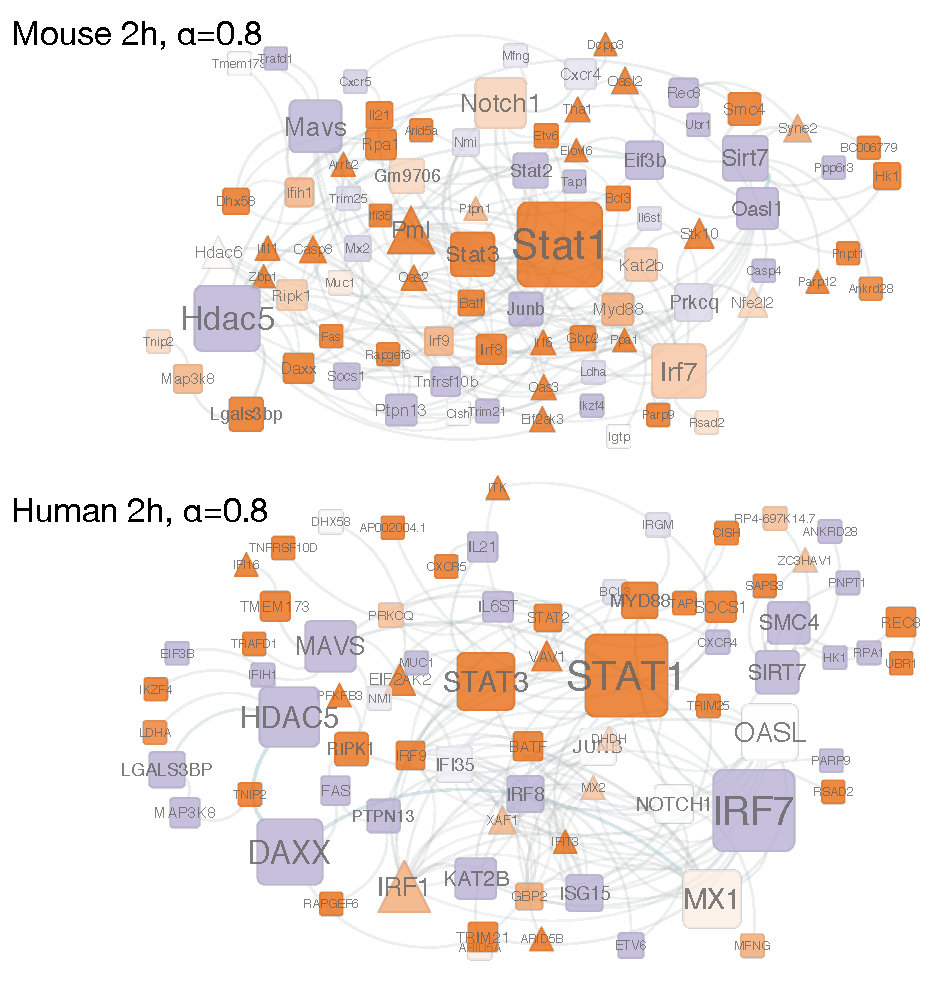
\includegraphics[width=\textwidth]{full_networks_2h.pdf}
  \caption{Full module at \unit{2}{h} for $\alpha = 0.8$ conservation ratio}
  \label{fig:full_1}
\end{figure}

\begin{figure}[p]
  \centering
  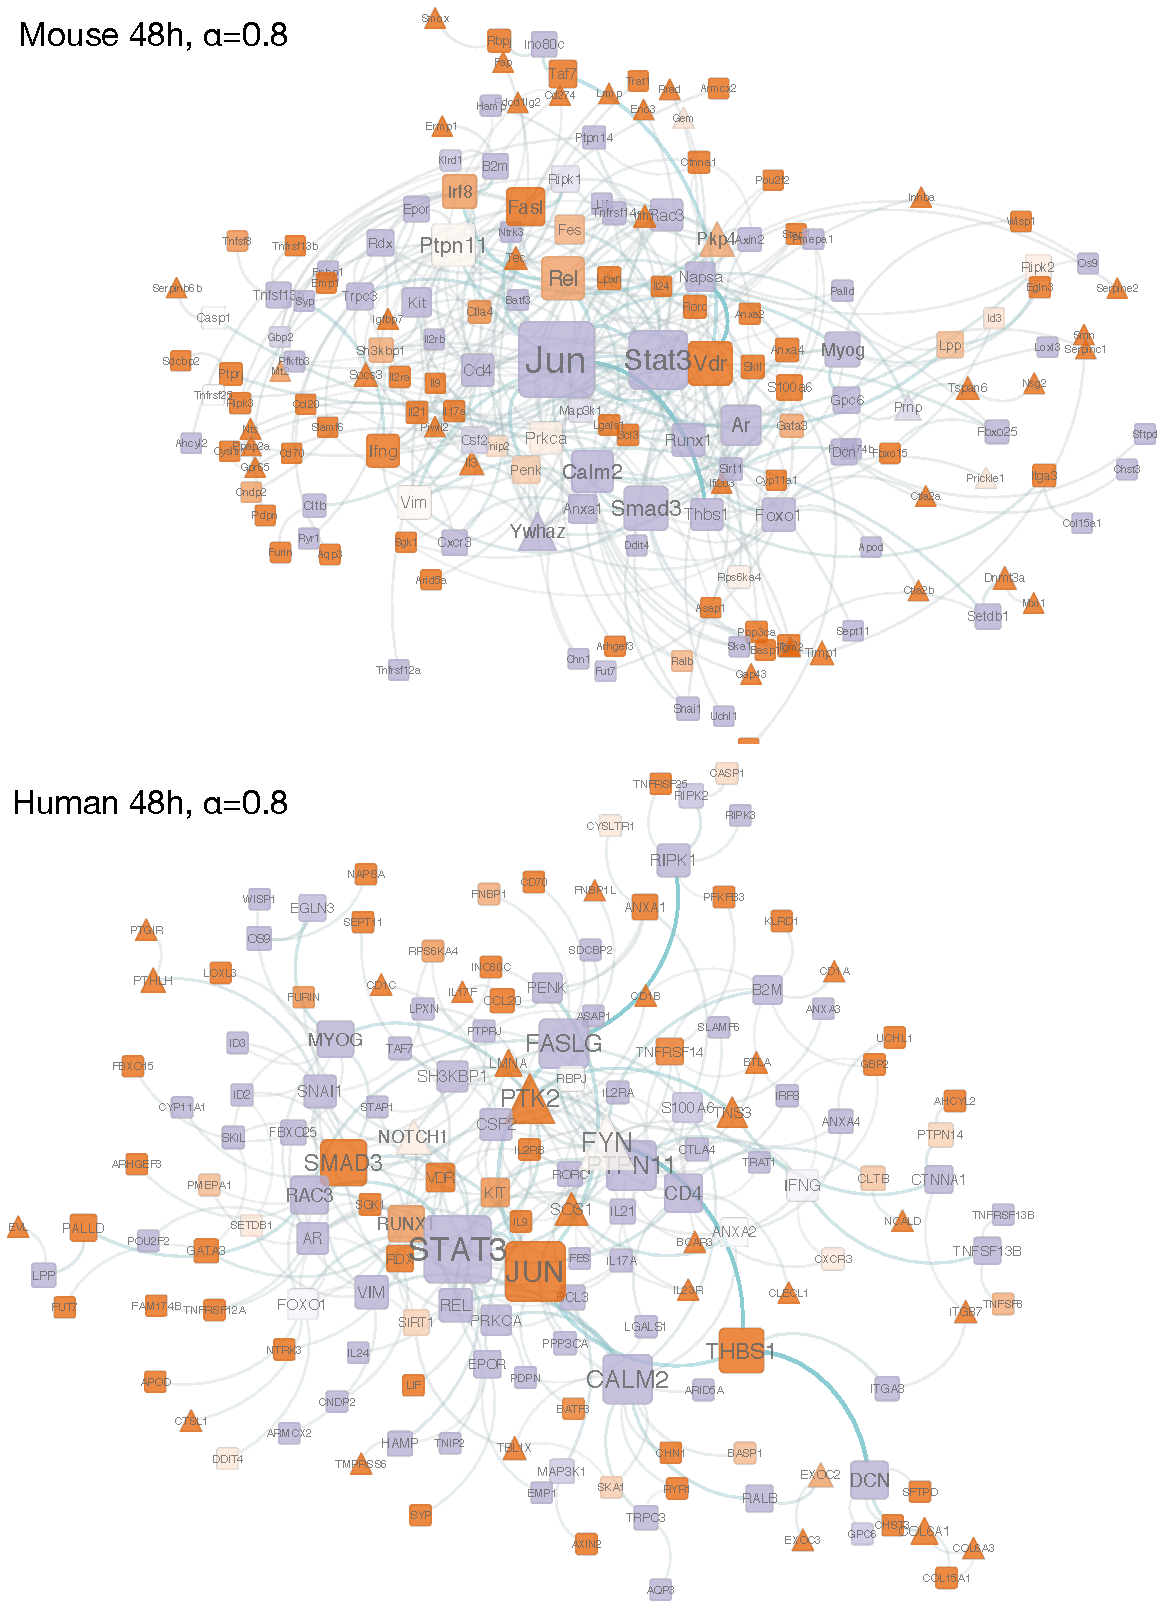
\includegraphics[width=\textwidth]{full_networks_48h.pdf}
  \caption{Full module at \unit{48}{h} for $\alpha = 0.8$ conservation ratio}
  \label{fig:full_2}
\end{figure}

% The parameter $\alpha$ represents as equilibrium between module's conservation
% and activity. We have evaluated if best conserved active modules show an
% increase in sequence similarity of selected proteins with an increase in
% $\alpha$. Indeed, sequence similarity is at the basis of most algorithms for
% identification of orthologous groups and in particular COGs. However, sequence
% similarity does not automatically imply function conservation. In particular,
% naive use of sequence similarity groups together dissimilar multi-domain proteins
% that share a common domain \citep{Smith:97}, and can be fooled by
% promiscuous domains \citep{Doolittle:95,Marcotte:99}. This was overcome
% in COGs construction by manual curation and indeed it is possible to have two
% orthologous genes with relatively low similarity (e.g., HERE THE LOWEST SCORE
% FOR COGS). Nevertheless, we observe that correcting for co-activity and
% co-conservation mostly preserves genes having high sequence similarity.

% TODO HERE SPECULATE??? We hypothesize here that high differential activity is
% mostly conserved between species for those genes that not only have similar
% domain architecture and function, but are highly similar in their sequences.

% subsection
% main_regulation_of_th17_differentiation_is_conserved_between_human_and_mouse
% (end)

\subsubsection{Comparison to \nexus{}}
\label{sec:Nexus}

We compare the \unit{48}{h} \xheinz{} modules (see \cref{fig:panel_wht-xheinz_modules,fig:full_1,fig:full_2}) with subnetworks computed by \nexus{} version 3 \parencite{deshpande2010scalable}.
In contrast to our exact approach, \nexus{} uses a heuristic technique to grow subnetworks from seed nodes simultaneously in two species in an iterative fashion.
Neighborhoods of the two current modules are determined using a depth-first search.
This search is restricted to only consider nodes that have a path to the seed node with a confidence larger than the user-specified parameter $\mathtt{dfscutoff}$.
The confidence of a path is defined as the product of the confidences of the edges comprising that path.
The modules are extended to include the most active pair of orthologous nodes in the neighborhoods -- where activity is defined as normalized log fold change and thus differs from the definition of activity used in \xheinz{}.
This whole procedure is repeated until either the cluster coefficient drops below the user-specified parameter $\mathtt{cc}$, or the average activity scores of one of the two modules drops below parameter $\mathtt{scorecutoff}$.

We ran \nexus{} with the default parameters $\mathtt{cc = 0.1,0.2}$, $\mathtt{scorecutoff=0.15}$ and $\mathtt{dfscutoff=0.3,0.8}$ for mouse and human respectively for all time points. \Cref{tab:nexus_all} gives the resulting modules sizes for human and mouse.

\begin{table}[h]
	\centering
	\makebox[0pt]{
	\scriptsize
	\tabcolsep=0.075cm
	\begin{tabular}{lp{7.4mm}p{7.4mm}p{7.4mm}p{7.4mm}p{7.4mm}p{7.4mm}p{7.4mm}p{7.4mm}p{7.4mm}p{7.4mm}p{7.4mm}p{7.4mm}p{7.4mm}p{7.4mm}p{7.4mm}lp{7.4mm}rp{7.4mm}}
	\hline
	solution & 1 & 2 & 3 & 4 & 5 & 6 & 7 & 8 & 9 & 10 & 11 & 12 & 13 & 14 & 15 & avg. & \#sols\\ \hline
	0.5h & 7 (6) & 4 (4) & 7 (6) & 3 (3) & & & & & & & & & & & & 5.25 (4.75) & 4\\
	1h & 15 (10) & 10 (9) & 12 (12) & 13 (13) & 7 (7) & 5 (5) & 15 (13) & 10 (11) & 9 (10) & 18 (16) & 25 (24) & 14 (14) & 6 (7) & 5 (5) & 6 (6) & 9.95 (9.58) & 19\\
	2h & 15 (17) & 6 (5) & 12 (10) & 12 (11) & 10 (10) & 13 (13) & 17 (15) & 12 (12) & 8 (9) & 5 (5) & 11 (12) & 19 (18) & 3 (3) & 9 (8) & 23 (21) & 10 (9.83) & 30\\
	4h & 6 (9) & 4 (4) & 6 (5) & 4 (4) & 4 (4) & 3 (3) & 7 (8) & 9 (10) & 4 (4) & 3 (3) & & & & & & 5 (5.40) & 10\\
	48h & 5 (5) & & & & & & & & & & & & & & & 5 (5) & 1\\
	\hline
	\end{tabular}
	}
	\caption[Modules calculated with \nexus{} for all time points]{\textbf{Modules calculated with \nexus{} for all time points.}
	Shown are the sizes in number of nodes of the first 15 representative solutions and the average sizes for the human subnetwork and for the mouse subnetwork in brackets.
	The last column lists the number of solutions for each time point.
	No solutions were obtained for time points \unit{24}{h} and \unit{72}{h}.
	}
	\label{tab:nexus_all}
\end{table}

\nexus{} finds 1 module for time point \unit{48}{h} which is shown in \cref{fig:nexus} for human (A) and mouse (B).
In total 5 genes are contained in the module, which are identical for human and mouse, but the number of edges differs.
Only one of the genes is significantly differentially expressed, CCL20, which has an absolute log fold change bigger than 1 and a BH FDR smaller than 0.1.
Since \nexus{} does not use p-values as an input, but log fold-changes which are normalized to activity values, the genes CCL20 and CXCR3 are considered as active nodes with a value above 0.15.
These genes show changes in expression, but only two of these changes are statistically significant.

The low number of active nodes points to a drawback in the \nexus{} algorithm: due to the locality of the greedy search strategy it may happen that the average activity of the subnetwork in construction keeps on degrading without reaching the next active node.
The effects of this issue can be seen, for example, in \cref{fig:nexus}, where CCL20 is the seed node and the majority of other neighboring nodes are not differentially expressed.
Furthermore, since the activity score of a single gene is just the log fold-change, and does not reflect both fold change and variability as a p-value, the neighboring nodes of the seed node in subnetwork \cref{fig:nexus} might merely originate from the noise in the data and represent nothing biologically relevant for the interpretation of the data.

\begin{figure}[h]
	\centering
	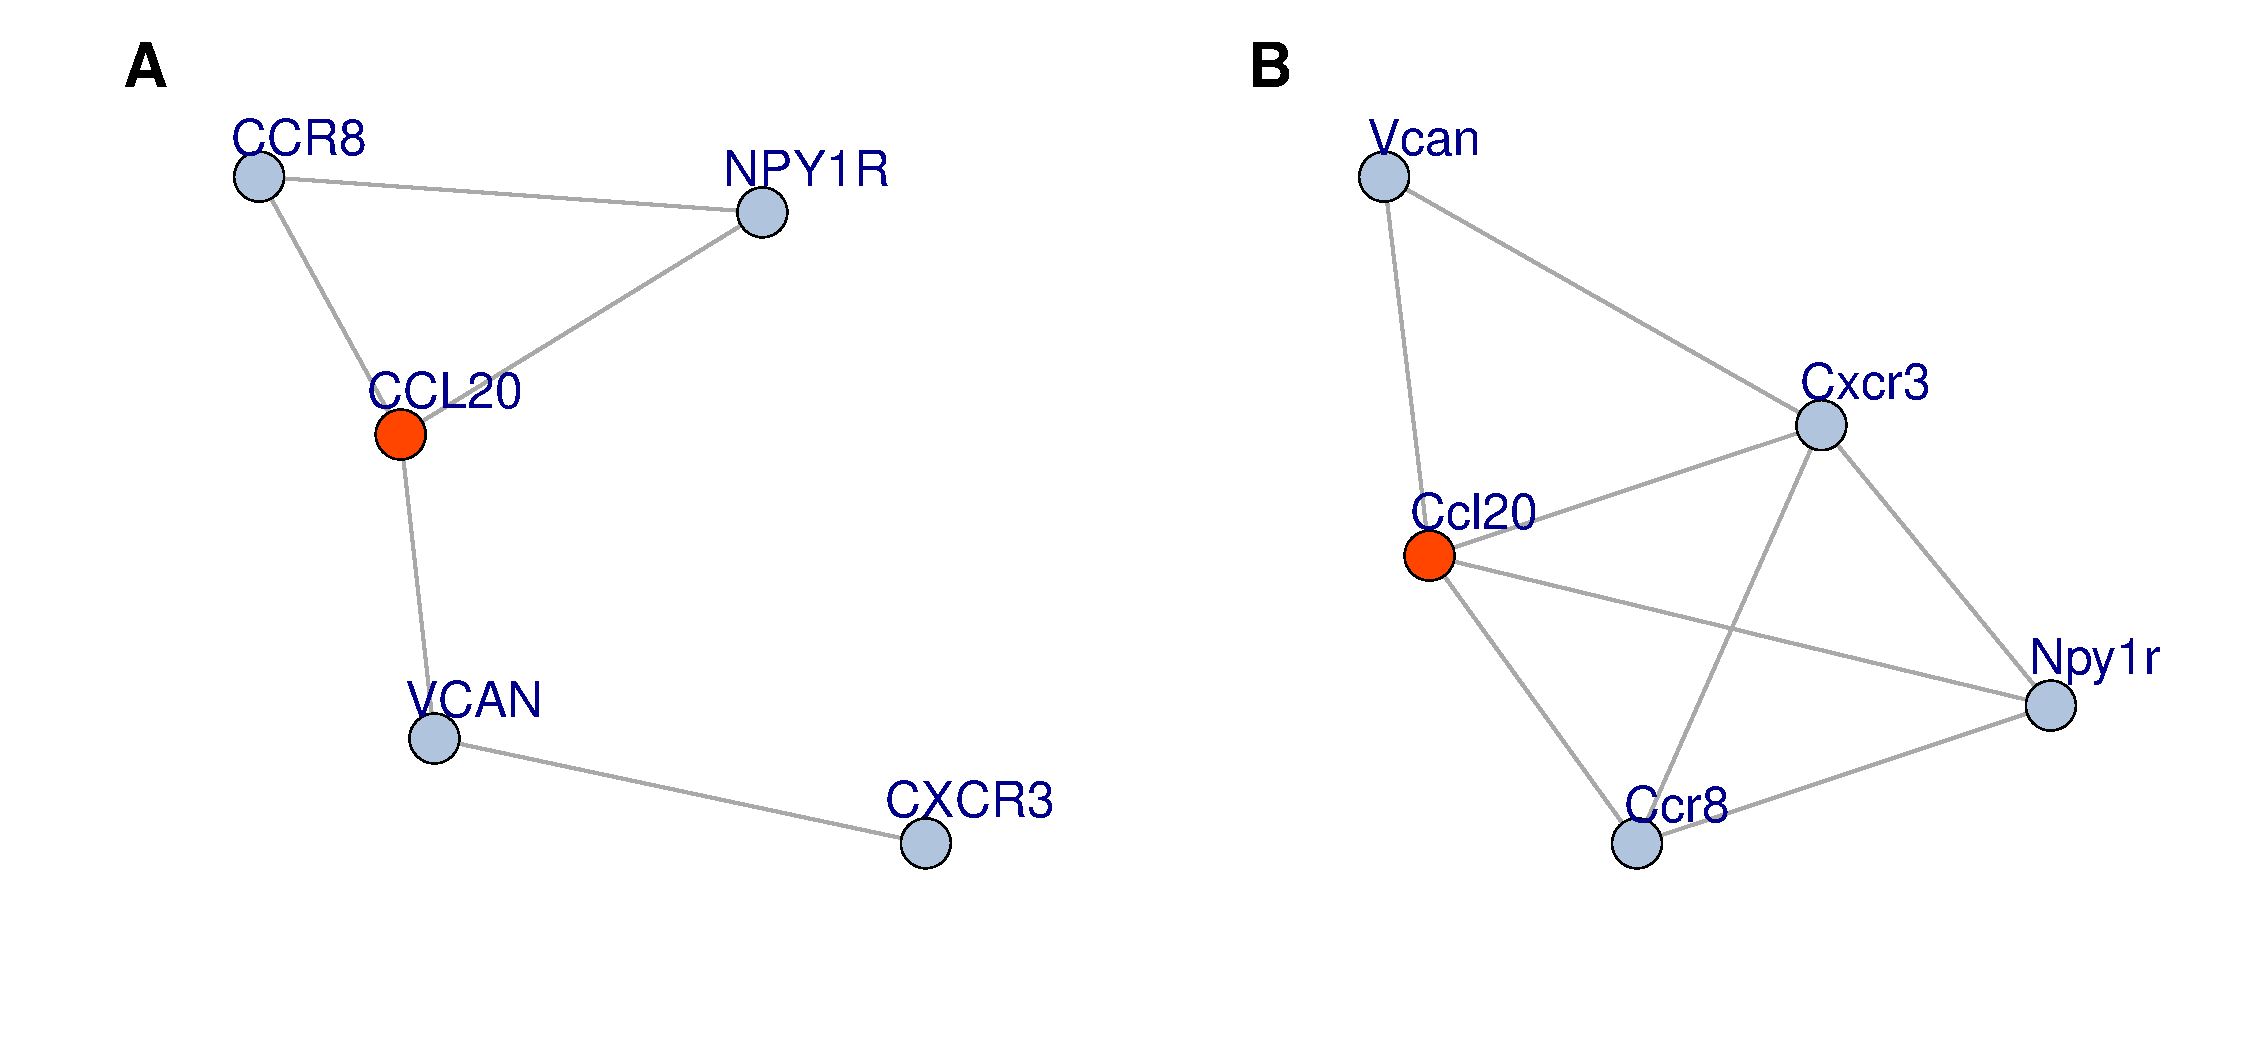
\includegraphics[width=\linewidth]{img/Nexus_module_A.pdf}
	\caption[\nexus{} modules for the time point 48 hours for human and mouse]{\textbf{\nexus{} modules for the time point 48 hours for human (A) and mouse (B).}
	Orange coloring indicates genes with significant differential expression (BH FDR $\leq 0.1$, $\absLOGFC \geq 1$).
	Here only one gene is significantly differentially expressed (CCL20).
	}
	\label{fig:nexus}
\end{figure}

\paragraph{}
Another consequence of the \nexus{} search strategy is that the module sizes are small (see \cref{tab:nexus_all}) and thus only give a limited view of the molecular mechanisms at play.
Theoretically, the parameter $\mathtt{dfscutoff}$ can be decreased to increase the module size.
Doing so, however, produces only slightly larger modules, but drastically increases the running time.
\Cref{tab:dfs} shows the \nexus{} solutions for time point \unit{48}{h} with different values for parameter \texttt{dfscutoff}.

\begin{table}[h]
	\caption[\nexus{} solutions for time point \unit{48}{h} with different values for parameter \texttt{dfscutoff}.]{\textbf{\nexus{} solutions for time point \unit{48}{h} with
    different values for parameter \texttt{dfscutoff}.} Shown are  the number of solutions, the average and maximum number of nodes and running times for the human network.}
\begin{center}
\tabcolsep=0.08cm
%\small
%%\color{red}
\begin{tabular}{lrrrrrrr}
\hline
dfscutoff & no.\ sols. & avg.\ size & max.\ size& CPU time [s] \\ \hline
0.1 & 2 & 5.00 & 5 & 176039.91\\
0.2 & 3 & 7.00 & 9 & 110282.61\\
0.3 & 5 & 6.60 & 9 & 77502.13\\
0.4 & 4 & 6.62 & 10 & 54972.92\\
0.5 & 6 & 5.58 & 9 & 35360.42\\
0.6 & 4 & 5.38 & 6 & 20538.4\\
0.7 & 3 & 5.33 & 6 & 11164.19\\
0.8 & 60 & 4.04 & 6 & 4639.59\\
0.9 & 0 & 0.00 & 0 & 1359.87\\ \hline
\end{tabular}
\end{center}
\label{tab:dfs}
\end{table}


Also note that changes in the clustering coefficient parameter $\mathtt{cc}$ only reduce the module size with increasing $\mathtt{cc}$.
\Cref{tab:cc} shows the \nexus{} solutions for time point \unit{48}{h} with different values for parameter \texttt{cc}.

\begin{table}[h]
	\caption[\nexus{} solutions for time point \unit{48}{h} with different values for parameter \texttt{cc}]{\textbf{\nexus{} solutions for time point \unit{48}{h} with
    different values for parameter \texttt{cc}.} Shown are  the number of solutions, the average and maximum number of nodes and running times for the human network.}
\begin{center}
\tabcolsep=0.08cm
%\small
%%\color{red}
\begin{tabular}{lrrrrrrr}
\hline
cc & no.\ sols. & avg.\ size & max.\ size& CPU time [s] \\ \hline
0.1 & 1 & 5 & 5 & 23367.68\\
0.2 & 1 & 5 & 5 & 23243.83\\
0.3 & 1 & 5 & 5 & 23903.09\\
0.4 & 1 & 5 & 5 & 24285.30\\
0.5 & 1 & 3 & 3 & 24318.78\\
0.6 & 1 & 3 & 3 & 24059.59\\
0.7 & 1 & 3 & 3 & 24518.68\\
0.8 & 1 & 3 & 3 & 24321.92\\
0.9 & 1 & 3 & 3 & 24246.56\\ \hline
\end{tabular}
\end{center}
\label{tab:cc}
\end{table}
%%}

\paragraph{}
Conservation in \nexus{} is enforced stringently by only allowing pairs of orthologous genes or genes that are only present in one of the networks to be included in the subnetworks (see \cref{fig:nexus}).
This is too restrictive if the underlying mechanisms in the two species differ.
For instance, for time point 48 hours and all but $\alpha=1$ values, \xheinz{} finds the non-conserved gene IL23R (BH FDR 3.52e-8, score 14.50, logFC 1.38) in human, which is involved in Th17 autocrine signaling \parencite{wei200721} but which is not differentially expressed in mouse.
\xheinz{} also finds JUNB, which at the 2 hour time point is up-regulated in human data (BH FDR 1e-2, score 0.02, logFC 1.3) and not detected as differentially expressed in the mouse data (BH FDR 0.48, score -4.01, logFC 0.65).
JUNB is a known partner of BATF with which it heterodimerizes preferentially during Th17 differentiation \parencite{schraml2009ap}, indicating its relevance.
Both important genes would have been missed by a more restrictive conservation setting.
Indeed, both \nexus{} and \xheinz{} at $\alpha = 1$ fail to find these genes showing that a more flexible view on conservation is required to adequately deal with transferability.

\section{Implementation and evaluation details}
	\subsection{Implementation}

	\xheinz{} is implemented in modern C++14 using the best practice patterns recently introduced by \textcite{meyers2014effective}, and makes use of the boost libraries and the LEMON graph library \parencite{dezsHo2011lemon}.
		CPLEX 12.6 is used as a black-box solver for our Mixed-Integer Linear Program formulation.
		The source code is publicly available in a git repository linked to from \mbox{\url{http://software.cwi.nl/xheinz}}.

		\paragraph{}
		Given two species, \xheinz{} takes as input:
		\begin{enumerate}
			\item a network for each of the species: $G_1$ and $G_2$,
			\item a mapping between the nodes of the two networks,
			\item scores associated to each of the nodes, \eg, derived from the p-value of the moderated t-test,
			\item the threshold value $\alpha$, and
			\item an optional time limit.
		\end{enumerate}

		\xheinz{} returns two node sets corresponding to a solution found within the time limit together with an upper bound on the optimal objective value.
		If the objective value equals this upper bound, the computed solution is provably optimal.

  \subsection{Data processing pipeline}
  The full pipeline, implemented using Snakemake, from data downloading to running xheinz, goes as follows:\pagebreak
  \begin{enumerate}
    \item Retrieve human and mouse ENSEMBL orthologs, STRING species specific network
    \item Retrieve human dataset from GEO (all time points, all conditions)
    \item Annotate human probes with ENSEMBL 
    \item Select human probes based on variance filter
    \item Perform linear modeling of the whole human dataset 
    \item Retrieve mouse dataset (all time points, all conditions)
    \item Annotate mouse probes with ENSEMBL 
    \item Select mouse probes based on variance filter
    \item Perform linear modeling of the whole mouse dataset 
    \item For each time point of interest: 
    \begin{enumerate}
      \item Call differentially expressed human genes by contrasting the Th17 with the Th0 condition $\Rightarrow$ p-value for each gene at this time point
      \item Call differentially expressed mouse genes by contrasting the Th17 with the Th0 condition $\Rightarrow$ p-value for each gene at this time point
      \item For an FDR threshold of 0.1, fit a BUM model for the human genes $\Rightarrow$ positive and negative scores for human genes
      \item For an FDR threshold of 0.1, fit a BUM model for the mouse genes $\Rightarrow$ positive and negative score for mouse genes 
      \item Rank normalize the mouse score based on the human scores $\Rightarrow$ update the scores of the mouse genes
      \item Map human and mouse genes to proteins on the STRING network
      \item For each value of interest for the conservation threshold $\alpha$:
      \begin{enumerate}
        \item Run xHeinz with the following inputs: 
        \begin{enumerate} 
          \item the human STRING network 
          \item the mouse STRING network
          \item the BUM scored human proteins
          \item the BUM scored mouse proteins
          \item the human and mouse orthologs
        \end{enumerate}
      \end{enumerate}
    \end{enumerate}
  \end{enumerate}

  \subsection{Significance of results}
  \label{app:significance}

  We computed empirical p-values to assess the significance of
  the obtained scores at \unit{2}{h} and \unit{48}{h}, for each value of
  $\alpha \in \{0.1, 0.2, \ldots, 1.0\}$, with the following two procedures:
  \begin{enumerate}
    \item \emph{Weights permutation:} We shuffled the node weights by generating random permutations of the activity scores of all genes.
    \item \emph{Topology permutation:} We repeated a million times the following operation: given two randomly selected edges A1--A2 and B1--B2, if the edges A1--B2 and B1--A2 are not present in the network we add them and remove the original edges, thus generating a random network with the same node weights and degree distribution.
  \end{enumerate}

  For each resulting permuted network we applied a modified version of xHeinz a
  fixed number of times (500 times for $\alpha = 0.8$, 100 times otherwise). This
  modified version allows to check whether the optimal score on the new random
  network would exceed the best score we found on the original network.

  To speed up these computations, we used the observation that solving a relaxed
  version of the conserved modules problem is sufficient, since we only need a
  sufficiently low upper bound (less than the score we obtained with unshuffled
  data) on the optimal values for those shuffled instances to make this decision.
  
  We therefore consider the following ILP for the shuffled instances:
  \allowdisplaybreaks
  \begin{alignat}{3}
   \label{eq:relaxed}\max\: & \sum_{v \in V_1 \cup V_2} w_v x_v \\
   \text{s.t.}\:\: & \eqref{eq:m_u}, \eqref{eq:m_v},
  \eqref{eq:b}, \eqref{eq:vars}
  \end{alignat}
  that is, we drop the connectivity constraints. Note that the objective
  value is an upper bound of the optimal score of the original problem
  since this new ILP is a relaxation of the original one. In
  addition, we can stop the branch-and-cut algorithm as soon as the
  upper bound on \eqref{eq:relaxed} is lower than the best found
  solution of the original ILP on the unshuffled data. These two
  observations help to speed up the significance computations tremendously.

  \Cref{tab:pval} shows the results of these runs, which we
  performed using a cumulative time limit of \unit{500}{h}. It can be seen that only
  at extreme values of $\alpha$ for the \unit{48}{h} time point the
  upper bound on \eqref{eq:relaxed} was not good enough to prove
  significance. This result was actually expected, since the original run was the only one
  with a very high gap ($33.36\%$) at the end of the allocated timelimit.

  Note that the p-values $\hat p$ that we demonstrate here are actually upper bounds to the
  underlying p-values $p$ that we would obtain without the relaxation to the ILP.

  For all other combinations, including the ones we chose to compute the Th17 modules
  and where we computed even more permutations, our procedure
  demonstrates that the signal in the real network is useful to obtain a
  statistically significant score.

  \begin{center}
  \begin{table}[h]
  \centering
  \tabcolsep=0.08cm
  {%\small
  \begin{tabular}{| c | c | c | c | c | c |}
  \hline
  Timepoint & $\alpha$ & FDR & $k$ & $k'$ & $\hat p$ \\ \hline
  \unit{2}{h}  & 0.1 & 0.1 & 100 & 0   & 0.0   \\
  \unit{2}{h}  & 0.2 & 0.1 & 100 & 0   & 0.0   \\
  \unit{2}{h}  & 0.3 & 0.1 & 100 & 0   & 0.0   \\
  \unit{2}{h}  & 0.4 & 0.1 & 100 & 0   & 0.0   \\
  \unit{2}{h}  & 0.5 & 0.1 & 100 & 0   & 0.0   \\
  \unit{2}{h}  & 0.6 & 0.1 & 100 & 0   & 0.0   \\
  \unit{2}{h}  & 0.7 & 0.1 & 100 & 0   & 0.0   \\
  \textbf{\unit{2}{h}}  & \textbf{0.8} & \textbf{0.1} & \textbf{500} & \textbf{0}   & \textbf{0.0}   \\
  \unit{2}{h}  & 0.9 & 0.1 & 100 & 0   & 0.0   \\
  \unit{2}{h}  & 1.0 & 0.1 & 100 & 0   & 0.0   \\ \hline
  \unit{48}{h} & 0.1 & 0.1 & 100 & 7   & \textbf{0.07}  \\
  \unit{48}{h} & 0.2 & 0.1 & 100 & 4   & \textbf{0.04}  \\
  \unit{48}{h} & 0.3 & 0.1 & 100 & 0   & 0.0   \\
  \unit{48}{h} & 0.4 & 0.1 & 100 & 0   & 0.0   \\
  \unit{48}{h} & 0.5 & 0.1 & 100 & 0   & 0.0   \\
  \unit{48}{h} & 0.6 & 0.1 & 100 & 0   & 0.0   \\
  \unit{48}{h} & 0.7 & 0.1 & 100 & 0   & 0.0   \\
  \textbf{\unit{48}{h}} & \textbf{0.8} & \textbf{0.1} & \textbf{500} & \textbf{0}   & \textbf{0.0}   \\
  \unit{48}{h} & 0.9 & 0.1 & 100 & 0   & 0.0   \\
  \unit{48}{h} & 1.0 & 0.1 & 100 & 100 & \textbf{1.0} \\
   \hline
  \end{tabular}}
  \qquad
  {%\small
  \begin{tabular}{| c | c | c | c | c | c |}
  \hline
  Timepoint & $\alpha$ & FDR & $k$ & $k'$ & $\hat p$ \\ \hline
  \unit{2}{h}  & 0.1 & 0.1 & 100 & 0   & 0.0   \\
  \unit{2}{h}  & 0.2 & 0.1 & 100 & 0   & 0.0   \\
  \unit{2}{h}  & 0.3 & 0.1 & 100 & 0   & 0.0   \\
  \unit{2}{h}  & 0.4 & 0.1 & 100 & 0   & 0.0   \\
  \unit{2}{h}  & 0.5 & 0.1 & 100 & 0   & 0.0   \\
  \unit{2}{h}  & 0.6 & 0.1 & 100 & 0   & 0.0   \\
  \unit{2}{h}  & 0.7 & 0.1 & 100 & 0   & 0.0   \\
  \textbf{\unit{2}{h}}  & \textbf{0.8} & \textbf{0.1} & \textbf{500} & \textbf{0}   & \textbf{0.0}   \\
  \unit{2}{h}  & 0.9 & 0.1 & 100 & 0   & 0.0   \\
  \unit{2}{h}  & 1.0 & 0.1 & 100 & 0   & 0.0   \\ \hline
  \unit{48}{h} & 0.1 & 0.1 & 100 & 7   & 0.0   \\
  \unit{48}{h} & 0.2 & 0.1 & 100 & 4   & 0.0   \\
  \unit{48}{h} & 0.3 & 0.1 & 100 & 0   & 0.0   \\
  \unit{48}{h} & 0.4 & 0.1 & 100 & 0   & 0.0   \\
  \unit{48}{h} & 0.5 & 0.1 & 100 & 0   & 0.0   \\
  \unit{48}{h} & 0.6 & 0.1 & 100 & 0   & 0.0   \\
  \unit{48}{h} & 0.7 & 0.1 & 100 & 0   & 0.0   \\
  \textbf{\unit{48}{h}} & \textbf{0.8} & \textbf{0.1} & \textbf{500} & \textbf{0}   & \textbf{0.0}   \\
  \unit{48}{h} & 0.9 & 0.1 & 100 & 0   & 0.0   \\
  \unit{48}{h} & 1.0 & 0.1 & 100 & 20  & \textbf{0.2} \\
   \hline
  \end{tabular}}
  \caption[Results of significance experiments]{Results of significance experiments. For $\alpha \in \{0.1, 0.2,
  	\ldots, 1.0\}$ at time points \unit{2}{h} and \unit{48}{h} we computed upper
  	bounds on $k$ instances with permuted scores using the procedures described
  	above (weights permutation on the left, topology permutation on the right).
  	In $k'$ of these cases, %after a cumulative time limit of \unit{500}{h}, the
  	resulting upper bound was not lower than the score of the best found
  	conserved active module on the original network, resulting in a p-value $p
  \leq \hat p = k'/k$. Values at the threshold $\alpha = 0.8$ we used to compute
  the Th17 modules and non-zero p-values are highlighted.}
  \label{tab:pval}
  \end{table}
  \end{center}

  \subsection{Robustness of modules for varying $\alpha$}

  Given two modules $V_1' \subseteq V_1$ and $V_2' \subseteq V_2$, the
  Jaccard index is defined as $(V_1' \cap V_2')/(V_1' \cup
    V_2')$. Fig.~\ref{fig:jaccard_alpha} shows for each time point the
  Jaccard index for all pairs of conservation ratios. For consecutive
  values of $\alpha$ we can see that the module contents do not change
  much.

  Fig.~\ref{fig:focus_plot} shows the human gene module contents for time
  point \unit{2}{h} for varying values of $\alpha$, one gene per
  line. Genes in the left panel (FALSE) are negatively scored, that is,
  they are not differentially expressed at an FDR of 0.1. Genes in the
  right panel (TRUE) have a positive score. Squares represent conserved genes,
  whereas triangles represent non-conserved genes. An \xheinz module
  solution is thus the set of genes marked with a square or
  triangle at a given value of $\alpha$. The coloring is as follows:
  \begin{itemize}
  \item Genes that are selected at all values of $\alpha$ or
    are coloured red. These are the core genes. 
  \item Genes that are selected at $\alpha=0$ (no conservation)
    but not at $\alpha = 1$ are green. 
  \item Genes that are selected by $\alpha=1$
    (strict conservation) but not at $\alpha=0$ are turquoise. 
  \item Genes that can only be picked by \xheinz (intermediate $\alpha$ values)
    are orchid.
  \end{itemize}

  This figure shows that a large fraction of genes
  only occur in an intermediate $\alpha$ regime (orchid
  color). Furthermore, the module content smoothly changes as $\alpha$
  varies, which illustrates the robustness of the approach. \xheinz thus
  allows the investigator to make an informed choice on the conservation
  of genes in the modules, which is not possible with methods assuming
  no or strict conservation.

  \begin{figure}[b]
    \centering
    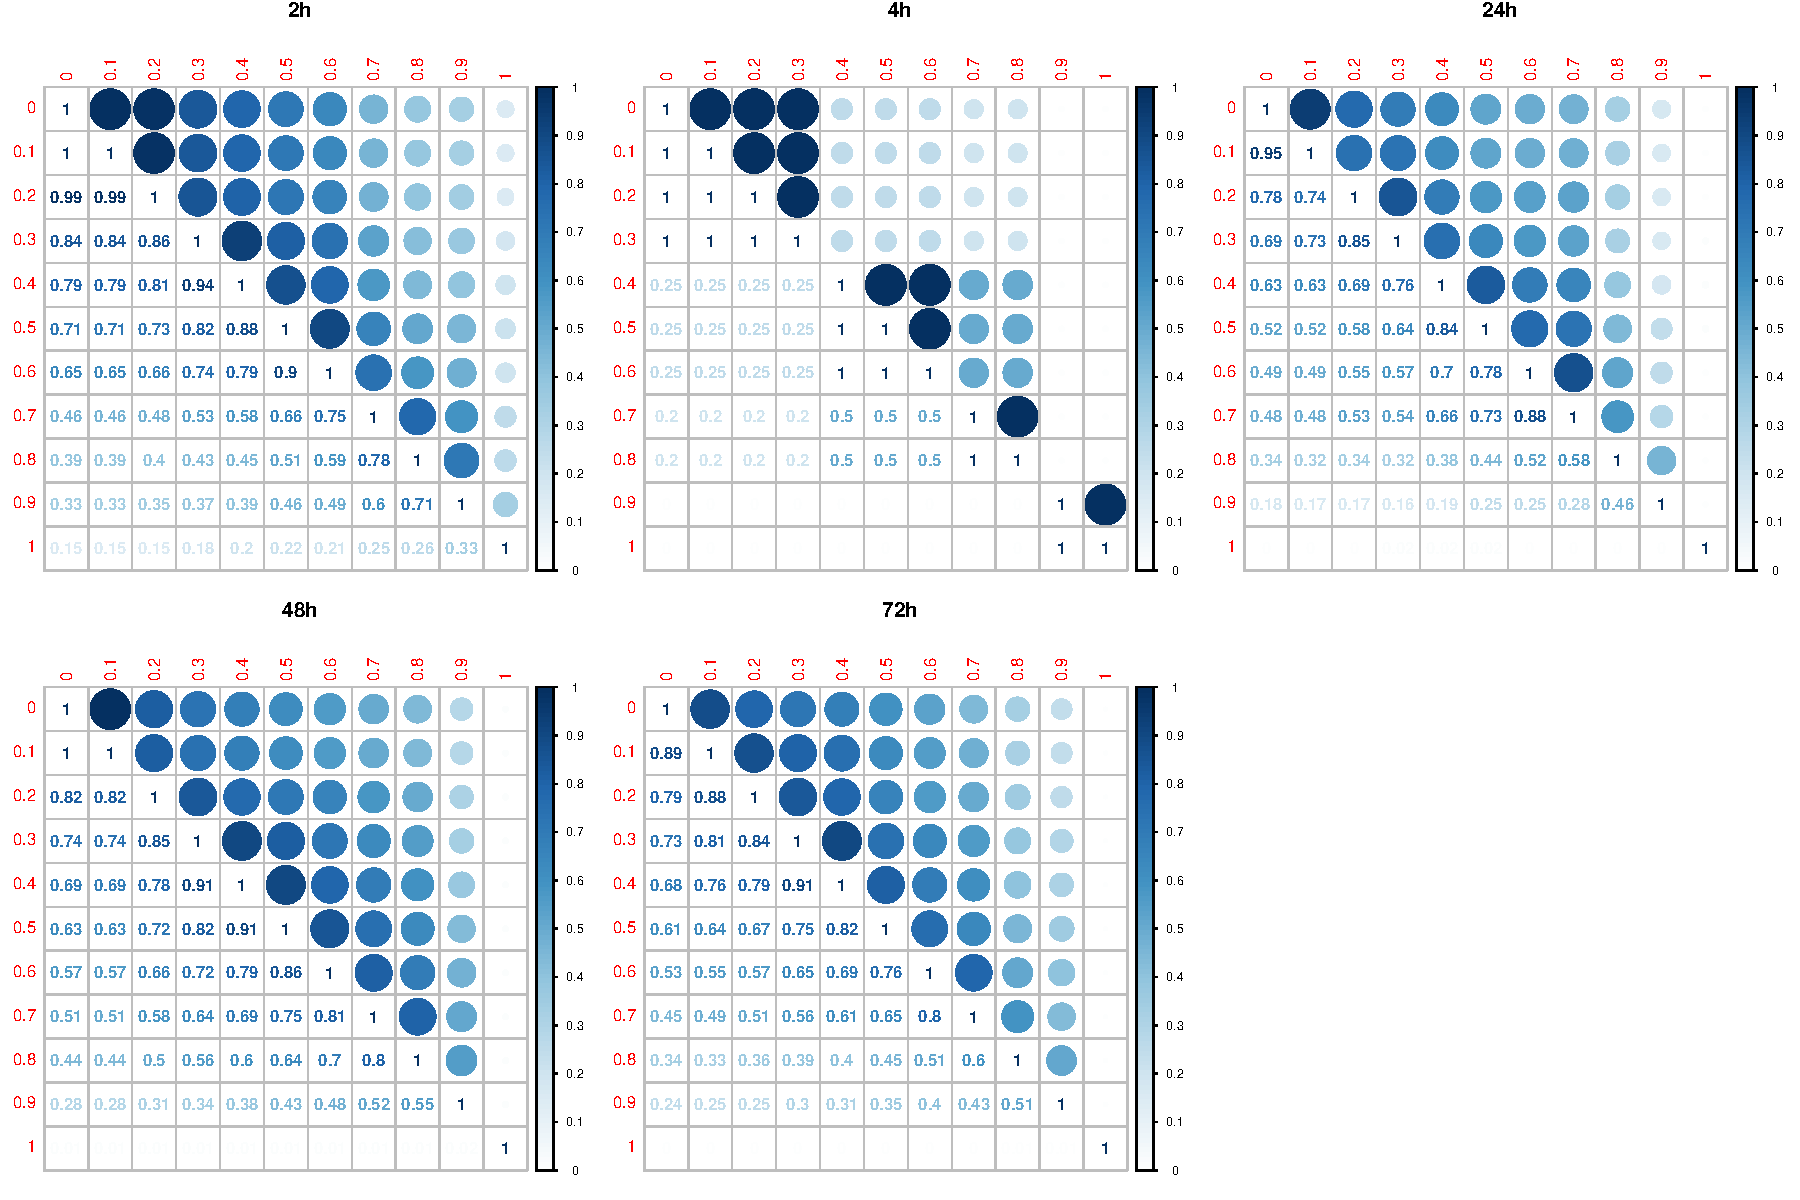
\includegraphics[width=1\linewidth]{jaccard_corrplot_numbers_v2.pdf}
    \caption{Jaccard index evolution over changes of $\alpha$}
    \label{fig:jaccard_alpha}
  \end{figure}

  \begin{figure}[p]
    \centering
    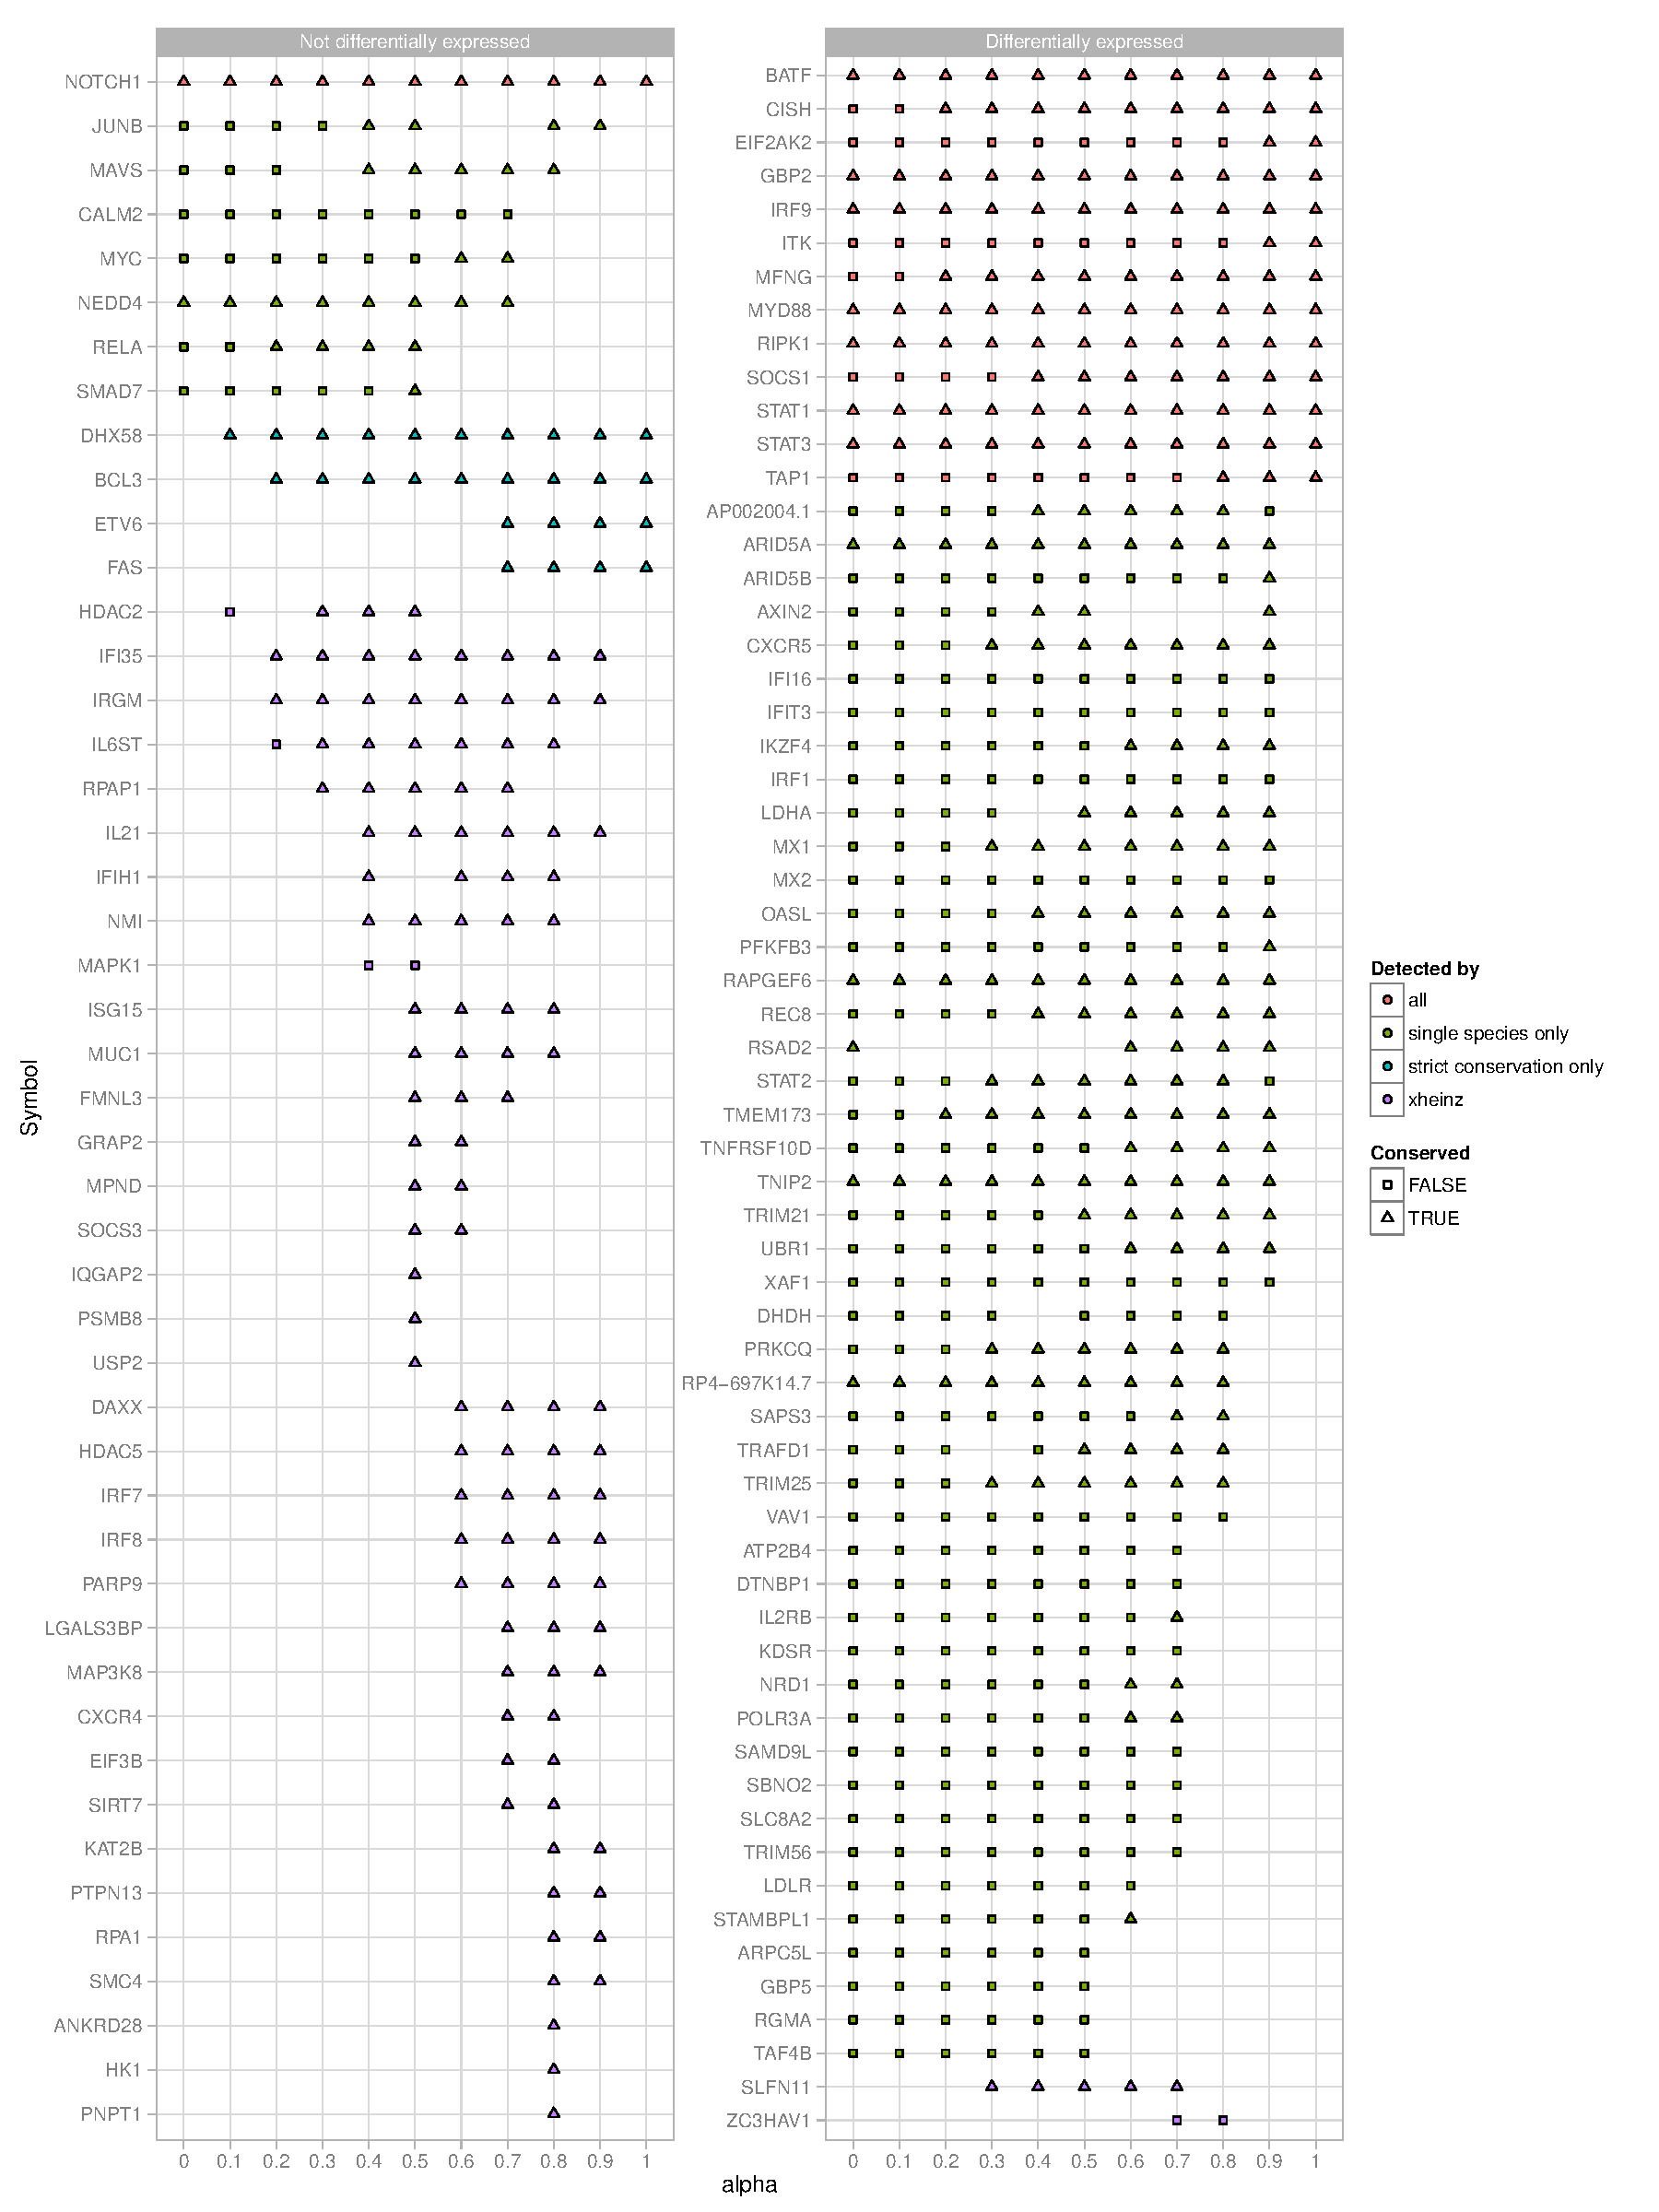
\includegraphics[width=1.2\linewidth]{focus_plot_2h_v2.pdf}
    \caption{Human module contents of the \unit{2}{h} time point with varying $\alpha$}
    \label{fig:focus_plot}
  \end{figure}

\section{Discussion}
\label{sec:xdisc}

We presented a module discovery method that simultaneously searches across two species for interesting gene sets.
A key feature of the gene sets that we extract is the guaranteed lower bound on the number of conserved genes that they contain.
This user defined lower bound, $\alpha \in [0, 1]$, provides a flexible conservation requirement between the two species, which allows for the discovery of conserved modules, including genes that would be missed with a stringent conservation requirement.%\footnote{Note that in the case of distantly-related species, a smaller $\alpha$ value may be more appropriate, which is a setup our model can be aptly applied to.}.
%In doing so, we thus contribute to the formalization of the notion of conserved active modules.

We have translated our model into an integer linear programming formulation and have devised and implemented an exact branch-and-cut algorithm that computes provably optimal or near-optimal conserved active modules in our model.

\paragraph{}
As a validation of our approach, our computational experiments for understanding the mechanisms underlying Th17 T cell differentiation in both mouse and human demonstrate that the flexibility in the definition of conservation is crucial for the computation of meaningful conserved active modules.
We have found two conserved Th17 modules at time points \unit{2}{h} ($\alpha = 0.8$) and \unit{48}{h} ($\alpha=0.8$) that thoroughly encompass the biphasic Th17 differentiation process.
This result can not be revealed by requiring full conservation ($\alpha = 1$) or by independent modules without requiring conservation ($\alpha = 0$).
Likewise, \nexus{}, an alternative approach based on a stringent conservation model, is not able to capture the key regulatory program of the differentiation process.

\paragraph{}
A key characteristics of our model is its flexibility.
This allows its extension to multiple species and time points, which we will address in future work.
In this case, however, realistic instances will be harder to compute to optimality.
Indeed, the number of interactions between multiple species or time points increase at least quadratically the number of both ILP variables and constraints.
It would requires the development of powerful algorithm engineering techniques.
Interestingly, the complexity of our branch-and-cut modelization of connectivity remains linear on the number of graphs involved.

%\paragraph{}
%It could be argued that gene conservation alone does not suffice to guarantee transferability.
%Indeed, recent studies in network alignment showed that biobjective models that look for both gene and interaction conservations tend to discover slightly different structures between species.
%
%However, since we deliberately opted for a constraint based representation of the conservation ratio\footnote{Instead of the more natural but problematic option of having the ratio as a free parameter to optimize for through the objective function.}, the model that we present in \ref{sec:mip} can be easily extended.
%Even though we specifically used a solver technique that does not model edges in the two graphs for performance reasons, there exists state of the art techniques that explicitly represent the edges, and that solve the \mwcs{} problem with competitive running times still (see chapter \emph{state of the art}).
%Using an explicit representation of the edges would allow for a very easy extension of our model.
%The interaction conservations would have to be explicitly represented in the inputs, for example with another bipartite graph linking edges in both graphs, and a conservation ratio constraint, similar to the one for genes, would be added to the integer model.
%
%Second, even though the mathematical model and the integer program are easy to modify, we decided to favor speed of execution in our current implementation.
%Indeed, the quality of most protein-protein interaction networks available is difficult to attest.
%Most of these networks are constructed using cross-species inferences, literature mining, and increasingly advanced techniques to statistically deduce protein interactions.
%We have found that filtering these networks for only the experimentally verified interactions results in most case in very sparse networks, which makes difficult any cross-species reasoning.

\paragraph{}
We presented a general model and its MIP program to solve any instance of the cross-species module discovery problem.
An extensive complexity analysis of the problem is presented in \cref{chap:hard}, where we show that some instances can be solved in polynomial time with specific algorithms.


%\part{Computational complexity}
\label{pt:3}

\chapter{Tight hardness bounds for the \mwccs{} problem}
\label{chap:hard}

	In this chapter, we outline the frontier of complexity that characterizes the \textsc{Maximum-Weight Cross-Connected Subgraph} (\mwccs{}) problem.
	We demonstrate that the bipartite relationship plays a major role in the separation between complexity classes, as do the types of input graphs.
	Furthermore, we provide constructive proofs, with algorithmic solution that efficiently solve some instances of the problem in polynomial time.

	The difficulty of the problem is not only dependent on the characteristics of the two main input graphs, but also of the relationship between the nodes of those two graphs.
	In \cite{hume2015approximation} we suggested that this characteristic is as important as those of the two graphs in defining the frontier of difficulty.
	We hypothesised that the problem might be polynomial-time solvable in some instances with a simpler relationship function.

	In \cref{sec:apx} we demonstrate that the \mwccs{} problem is inapproximable\footnote{NP-hard to approximate.} up to any arbitrary factor $\sigma < 1.0014$, it is thus an APX-hard problem.
	Exactly, we show that the APX-hardness holds for all inputs complex enough to represent the following cases:
	\begin{enumerate}
		\item one of the two graphs is a \emph{binary caterpillar tree}, the other a \emph{binary tree}, and the bipartite relationship is \emph{injective},
		\item one of the two graphs is a \emph{binary tree}, the other a general \emph{graph}, and the bipartite relationship is \emph{bijective}.
	\end{enumerate}
	\Cref{subsec:apx-bt-cater} contains the first proof.
	\Cref{subsec:apx-t-graph} contains the second proof for a tree and a general graph, and \cref{subsubsec:binary-tree} describe the scheme to extend the proof for a binary tree.

	\Cref{sec:poly} is separated into two main subsections dedicated to polynomially solvable cases of the \mwccs{}, both using constructive algorithmic description and with sub-problem definition and reduction.
	In \cite{hume2015approximation} we suggested that the problem might be solvable in polynomial time when both graphs are \emph{trees} and the relationship is \emph{bijective}; we give a proof for this conjecture in \cref{subsec:tree1o1}.
	This is important in that it draws a clear complexity frontier, distinctly dependent on the bipartite relationship.
	Finally, in \cref{subsec:enumerable} we provide a general algorithm to solve \mwccs{}.
	Doing so we introduce a new problem, \rbmwcs{}, to which \cref{sec:rbmwcs} is dedicated.
	Given that one of the two graphs is polynomially enumerable, we provide an efficient reduction from an \mwccs{} instance to a polynomial number of \rbmwcs{} instances.
	In this situation, \mwccs{} is thus as difficult as \rbmwcs{}: it is solvable in polynomial time when the second graph has a bounded treewidth\footnote{see \cref{subsec:enumerable} for the problem reduction and \cref{chap:rbmwcs} for the \rbmwcs{} hardness analysis.}.

	The exploration of the frontier of complexity is done in a similar fashion in the two contexts.
	Adding constraints on one hand leads to a relaxation of some other on the other hand, in order to stay within the same category of difficulty.
	In the hardness proof context, changing from an injective to a bijective mapping function requires that one of the two trees becomes a general graph for the problem to stay difficult.
	In the polynomial-time algorithms context, requiring that one of the graph that was previously a binary tree becomes more general%\footnote{In our case, we know it to be solvable for bounded treewidth, but it might be for more general classes of graphs too.}
	requires that the other becomes polynomially enumerable to stay solvable\footnote{In polynomial time.}.
	
	\section{APX-hardness of the \mwccs{} problem}
	\label{sec:apx}

		In this section we prove the inapproximability of two specific cases of the \mwccs{} problem.
		First, we prove that if the mapping between $G_1$ and $G_2$ is an injective function, if $G_1$ is a binary caterpillar tree, and if $G_2$ is a binary tree, \mwccs{} is APX-hard and can not be approximated within factor $1.0014$.
		Then, we prove that if the mapping is a bijective function, the problem is as hard to approximate as when considering a binary tree and a graph.
		These results in themselves shade some light on the role of the relationship function with respect to the difficulty of the problem.

		Both proofs consist in L-reductions from the APX-hard \msat{} problem (see \cref{par:m3sat}).

		%  In the next sections, we assume the following conventions: the variables are denoted by their indice $i$, $1 \leq i \leq n$, and we denote a valuation with the use of $+$ (resp. $-$) as the positive (resp. negative) valuation, followed by the indice of the variable.  We use $\circ$ as a shorcut for either one of the two valuations.  We note $N_{\circ,i}$ the number of clauses where the $\circ$ valuation of the $i$-th variable appears\footnote{we have $0 < N_{\circ,i} \leq 3$ since $F$ is a \cnf{} formula}.

		\subsection{Injective relationship function, binary trees}
		\label{subsec:apx-bt-cater}

		\begin{proposition}\label{prop:apx-bt-cater}
			The \mwccs{} problem for a binary caterpillar tree and a binary tree is APX-hard and not approximable within factor $1.0014$ even when the mapping $M$ is an injective function and a complete conservation (i.e. $\alpha = 1$) is required.
		\end{proposition}

		We first describe how we build an instance of \mwccs{} corresponding to an instance of \msat{}. Given any instance $(C_q,V_n)$ of \msat{}, we build a binary caterpillar tree $G_1=(V_1,E_1)$ with weight function $w_1$, a binary tree $G_2=(V_2,E_2)$ with weight function $w_2$, and a mapping $M$ as follows.

		The binary caterpillar graph $G_1$ is defined as follows. The vertex set is $V_1=\{r, l_i, c_j, dl_i, $ $dc_j ~\vert~$ $ 1\leq i\leq n, 1\leq j \leq q\}$. The edge set is given by the following equation.
		\begin{align*}
		E_1= &\{(c_j,dc_j), (l_i,dl_i) ~\vert~ 1\leq i\leq n, 1\leq j \leq q\}~\cup \\
		&\{(dc_q,r), (r,dl_1)\} \cup \\
		& \{(dc_j,dc_{j+1}), (dl_i,dl_{i+1}) ~\vert~ 1\leq i< n, 1\leq j < q\}.
		\end{align*}
		The weight function $w_1$ is defined as follows: for all $1 \leq i\leq n$ and $1\leq j \leq q$, $w_1(l_i)=B$, $w_1(c_j)=1$ and $w_1(r)=w_1(dc_j)=w_1(dl_i)=0$.

		Roughly, in $G_1$ there is a node for each clause (denoted by $c_j$) and for each literal (denoted by $l_i$) that represent the leaves of the caterpillar. The spine of the caterpillar contains dummy nodes for each clause (denoted by $dc_j$) and for each literal (denoted by $dl_i$) separated by a central node (denoted by $r$).

		The binary tree $G_2=(V_2,E_2)$ with weight function $w_2$ is defined as follows. The vertex set is $V_2=\{r, x_i, \overline{x_i}, c^k_j, dx_i, d\overline{x_i}, dc^i_j, dc^{\overline{i}}_j ~\vert~ 1\leq i\leq n, 1\leq j \leq q, 1\leq k\leq 3\}$. The edge set $E_2$ is given by the following equation.
		\begin{align*} E_2 = &\{(r,dx_n)\}~ \cup \\
			&\{(c^{k'}_j,dc^k_j) ~\vert~ x_k ,\text{is the } k' \text{-th literal of clause } c_j\}~ \cup \\
			&\{(c^{k'}_j,dc^{\overline{k}}_j) | \overline{x_k} ,\text{is the } k' \text{-th literal of clause } c_j\} ~\cup \\
			& \{ (dx_i,d\overline{x_{i+1}}) | 1\leq i < n\} ~\cup  \\
			& \{(dx_i,d\overline{x_i}), (dx_i, x_{n-i+1}), (d\overline{x_i},\overline{x_{n-i+1}}), (x_i,dc^i_1), (\overline{x_i},dc^{\overline{i}}_1) | 1 \leq i \leq n\}~ \cup  \\
			& \{(dc^i_j,dc^i_{j+1}), (dc^{\overline{i}}_j,dc^{\overline{i}}_{j+1}) | 1 \leq i \leq n, 1 \leq j < q\}
		\end{align*}

		The weight function $w_2$ is defined as follows:  for all $1\leq i\leq n$, $1\leq j \leq q$ and $1\leq k\leq 3$, $w_2(x_i)=w_2(\overline{x_i})=-B$ and $w_2(r)=w_2(c^k_j)=w_2(dx_i)=w_2(d\overline{x_i})=w_2(dc^i_j)=w_2(dc^{\overline{i}}_j)=0$ 

		Roughly, in $G_2$ there is a node for each literal of each clause (denoted by $c^k_j$) and for each value of each literal (denoted by $x_i$ and $\overline{x_i}$). Dummy nodes for literals have been duplicated (one for each value of the literal - that is $dx_i$ and $d\overline{x_i}$). Dummy nodes for clauses have also been duplicated (one for each value of all literals - $dc^i_j$ and $dc^{\overline{i}}_j$). The structure is not as easy to informally describe as for $G_1$ but the reader may refer to an illustration provided in Figure \ref{fig:bt-cater}.

		Finally, the mapping $M$ is an injective function from $V_1$ to $V_2$ defined as follows.
		\begin{align*}
			M(r)    &= r\\
			M(l_i)  &= \{x_i,\overline{x_i}\}, \text{for all } 1 \leq i\leq n\\
			M(c_j)  &= \{c^k_j|1\leq k\leq 3 \}, \text{for all } 1 \leq j \leq q\\
			M(dl_i) &= \{dx_i, d\overline{x_i}\}, \text{for all } 1 \leq i\leq n\\
			M(dc_j) &= \{dc^i_j, dc^{\overline{i}}_j\}, \text{for all } 1 \leq i\leq n \text{ and } 1 \leq j \leq q
		\end{align*}

		\begin{figure}[ht]
    	 	 \centering
    	 	 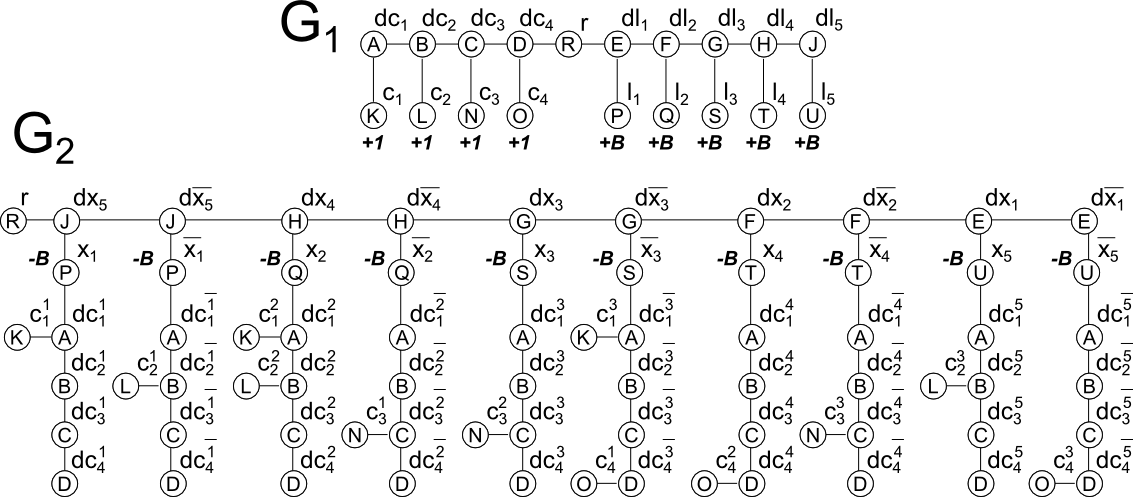
\includegraphics[width=\textwidth]{apx_bt-cater}
    	 	 \caption{XXX refaire avec TikZ si temps le permet XXX Illustration of the construction of $G_1$, $G_2$, and $M$, given $C_q = \{(x_1 \vee x_2 \vee \neg{}x_3), (\neg{}x_1 \vee x_2 \vee x_5), (\neg{}x_2 \vee x_3 \vee \neg{}x_4), (\neg{}x_3 \vee x_4 \vee \neg{}x_5)\}$. For readability, the mapping $M$ is not drawn but represented as labels located on the nodes: any pair of nodes (one in $G_1$ and one in $G_2$) of similar inner label are mapped in $M$.}
			\label{fig:bt-cater}
		\end{figure}

		Let us prove that this construction is indeed an L-reduction from \msat{}. More precisely, we prove the following property.
		\begin{lemma}
		There exists an assignment of $V_n$ satisfying at least $m$ clauses of $C_q$ if and only if there exists a solution to \mwccs{} of weight at least $m$.
		\end{lemma}

		\begin{proof}
		{\parindent0pt
		$\boxed{\Rightarrow}$ Given} an assignment $\mathcal{A}$ of $V_n$ satisfying $m$ clauses of $C_q$, we construct a solution to \mwccs{} of weight $m$ as follows.

		\begin{align*}
		\text{Let }V_1^*= &V_1 \setminus \{c_j ~\vert~ c_j\ \text{is not satisfied by the assignment}\}\text{ and}\\
		V_2^*= & \{r\} ~\cup \\
		& \{c^k_j ~\vert~ c_j \text{is satisfied by its } k\text{-th literal}\}  ~ \cup \\
		& \{x_i, dc^i_j ~\vert~ x_i=1, 1 \leq j \leq q\} ~\cup \\
		& \{\overline{x_i}, dc^{\overline{i}}_j ~\vert~ x_i=0, 1 \leq j \leq q\} ~\cup \\
		& \{dx_i,d\overline{x_i} ~\vert~ 1 \leq i \leq n\}.
		\end{align*}

		By construction, $G_1[V_1^*]$ is connected since all the vertices of the spine of the caterpillar have been kept. Moreover, $G_1[V_1^*]$ contributes $B \times n+m$ to the overall weight of the solution, that is $B$ for each of the $l_i$ and $+1$ for each satisfied clause.
		By construction, all the sub-trees rooted at $x_i$ (resp. $\overline{x_i}$) are kept in $G_2[V_2^*]$ if $x_i=1$ (resp. $x_i=0$) in $\mathcal{A}$. Moreover, all the dummy nodes for literals ($dx_i$ and $d\overline{x_i}$) and the root $r$ have been kept. Thus, $G_2[V_2^*]$ is also connected.
		Furthermore, $G_2[V_2^*]$ contributes to $-B\times n$ to the overall weight of the solution since exactly one of each variable node ($x_i$ and $\overline{x_i}$) has been kept. 
		One can easily check that any node of $V_1^*$ has a mapping counterpart in $V_2^*$. The overall solution is valid and of total weight $m$.

		\vspace*{1em}
		{\parindent0pt
		$\boxed{\Leftarrow}$ Given any solution $\{V_1^*,V_2^*\}$ to \mwccs{} of weight $m$, we construct a solution to the \msat{} problem satisfying at least $m$ clauses as follows.
		}

 	 	 First, note that we can assume that any such solution to \mwccs{} is \textit{canonical}, meaning that $V_2^*$ does not contain both vertices $x_i$ and $\overline{x_i}$ for all $1\leq i\leq n$. Indeed, by contradiction, suppose there exists a solution such that $\{x_i,\overline{x_i}\}\subseteq V_2^*$ for a given $1\leq i \leq n$. Then, $\{x_i,\overline{x_i}\}$ in $G_2$ induce a negative weight of $-2B$. This negative contribution can at most be compensated by the weight of the corresponding literal node in $G_1$ ($w_1(l_i)=B$) and at most $B$ clause nodes in $G_1$ ($B \geq \sum w_1(c_j)$ where $x_i\in c_j\ or\ \overline{x_i}\in c_j$) since every literal occurs in at most $B$ clauses in $C_q$. Therefore, such local configuration does not provide any positive contribution to the solution and can be transformed into a better solution by removing one of the sub-trees rooted in $\{x_i,\overline{x_i}\}$. We will consider hereafter that $m$ is the weight of the resulting canonical solution. We further assume that $m>1$ since otherwise we can build a trivial assignment $\mathcal{A}=\{c^1_1=1\}$ of $V_n$ that is satisfying at least one clause of $C_q$.

		Let $\mathcal{A}$ be an assignment of $V_n$ such that for all $1\leq i\leq n$ if $x_i\in V_2^*$ then $x_i=1$ and $x_i=0$ otherwise. Note that, since our solution is canonical, each literal has been assigned a single boolean value in $\mathcal{A}$. Let us now prove that this assignment satisfies at least $m$ clauses of $C_q$.

		First, note that since our solution is canonical and we require any node of $V_1^*$ to have a mapping counterpart in $V_2^*$, this implies that if $l_i\in V_1^*$ then its contribution (that is $w_1(l_i)=B$) is cancelled by the negative contribution of either $x_i$ or $\overline{x_i}$ in $V_2^*$ (that is $w_2(x_i)=w_2(\overline{x_i})=-B$). Therefore, the weight $m$ of the solution can only be realized by $m$ clause nodes of $G_1$, say $\mathcal{C}_1\subseteq V_1^*$ -- since $w_1(c_j)=1$ for all $1\leq j \leq q$.

		As already stated, to be part of the solution any node in $V_1^*$ has a mapping counterpart in $V_2^*$. Thus, for each node in $\mathcal{C}_1$, there should be a node of $\mathcal{C}_2 \subseteq \{c_j^k ~\vert~ 1\leq j \leq q, 1\leq k\leq 3\}$ in $V_2^*$. More precisely, by construction, any node $c_j$ in $V_1$ has exactly three mapping counterparts in $V_2$ (that is $\{c_j^k ~\vert~ 1\leq k \leq 3\}$) and for each $c_j\in \mathcal{C}_1$ at least one of these mapping counterparts has to belong to $\mathcal{C}_2$.

		Finally, since both $G_1[V_1^*]$ and $G_2[V_2^*]$ have to be connected, each node in $\mathcal{C}_2$, say $c_j^k$, should be connected by a path to a node $x_i$ or $\overline{x_i}$, say $x_i$, for some $1\leq i \leq n$, in $G_2[V_2^*]$. By construction, this is the case if $x_i$ is the $k$-th literal of the clause $c_j$ for some $1\leq k \leq 3$. Thus, $\mathcal{A}$ is an assignment that satisfies any clause $c_j$ such that the clause node $c_j$ belongs to $V_1^*$. As already stated $|\mathcal{C}_1|=m$.
		\end{proof}

		The above reduction linearly preserves the approximation since the weights of optimal solutions of the problems correspond and there exists an assignment of $V_n$ satisfying at least $m$ clauses of $C_q$ if and only if there exists a solution to \mwccs{} of weight at least $m$. Hence, given an approximation to \mwccs{}, one can derive an algorithm for \msat{} with the same approximation ratio. Since \msat{}, $B\geq 3$, is APX-hard \cite{papadimitriou1991optimization} and \msat{} for $B=6$ is not approximable within factor $1.0014$ \cite{berman1999some}, so is \mwccs{}, which proves \cref{prop:apx-bt-cater}.

		Let us now prove a similar result for \mwccs{} problem when the mapping is a bijective function.


		\subsection{Bijective relationship function, tree, and graph}
		\label{subsec:apx-t-graph}

		\begin{proposition}\label{prop:apx-t-graph}
  	  	  The \mwccs{} problem for a graph and a tree is APX-hard and not approximable within factor $1.0014$ even when the mapping is a bijective function and a complete conservation (i.e. $\alpha = 1$) is required.
		\end{proposition}

		Given any instance $(C_q,V_n)$ of \msat{}, we build a graph $G_1=(V_1,E_1)$ with weight function $w_1$, a tree $G_2=(V_2,E_2)$ with weight function $w_2$ and a mapping $M$ as follows. The graph $G_1$ has the vertex set $V_1=\{r, l_i, x_i, \overline{x_i}, c_j,$ $ c^k_j ~\vert~ 1\leq i\leq n, 1\leq j \leq q, 1\leq k \leq 3\}$ and the edge set defined by the following equation.
		\begin{align*}
		E_1= & \{(l_i,x_i), (l_i,\overline{x_i}), (r,x_i), (r,\overline{x_i}) ~\vert~ 1\leq i\leq n\} ~\cup  \\
 	 	 & \{(c_j,c_j^k), (r,c_j^k)  ~\vert~ 1\leq k \leq 3, 1\leq j \leq q\}.
		\end{align*}

		The weight function $w_1$ is defined as follows: for all $1\leq k \leq 3$, $1\leq i\leq n$ and $1\leq j \leq q$, $w_1(l_i)=B$, $w_1(c_j)=1$ and $w_1(r)=w_1(c_j^k)=w_1(x_i)=w_1(\overline{x_i})=0$.

		Roughly, in $G_1$ there is a node for each clause (denoted by $c_j$), for each of the three literals of each clause (denoted by $c_j^k$), for each literal (denoted by $l_i$) and for each valuation of each literal (denoted by $x_i$, $\overline{x_i}$). Clause nodes and literal nodes are separated by a central node $r$.

		The tree $G_2$ is defined as follows. The vertex set is $V_2=V_1$, the edge set is given by the following equation:
		\begin{align*}
		E_2= & \{(l_i,r), (c_j,r), (x_i,r), (\overline{x_i},r) ~\vert~ 1\leq i\leq n, 1\leq j \leq q\} ~\cup \\
		& \{(c^k_j,x_i) ~\vert~ x_i \text{ is the  } k\text{-th literal of clause } c_j\} ~\cup\\
		& \{(c^k_j,\overline{x_i}) ~\vert~ \overline{x_i} \text{ is the } k\text{-th literal of clause } c_j\}.
		\end{align*}

		The weight function $w_2$ is defined as follows: for all $1\leq k \leq 3$, $1\leq i\leq n$ and $1\leq j \leq q$, $w_2(x_i)=w_2(\overline{x_i})=-B$, $w_2(r)=w_2(c_j^k)=w_2(l_i)=w_2(c_j)=0$.


		Roughly, in $G_2$ all the nodes except the ones in $\{c_j^k~\vert~ 1\leq j \leq q, 1\leq k\leq 3\}$ form a star centered in node $r$. The nodes representing the literal of the clause (that is $c_j^k$) are connected to their corresponding variable nodes (that is $x_i$ or $\overline{x_i}$).

		Finally, the mapping $M$ is a bijective function from $V_1$ to $V_2$ defined as the identity (that is each node in $V_1$ is mapped to the node of similar label in $V_2$).


		\begin{figure}[ht]
    	 	 
    	 	 \centering
    	 	 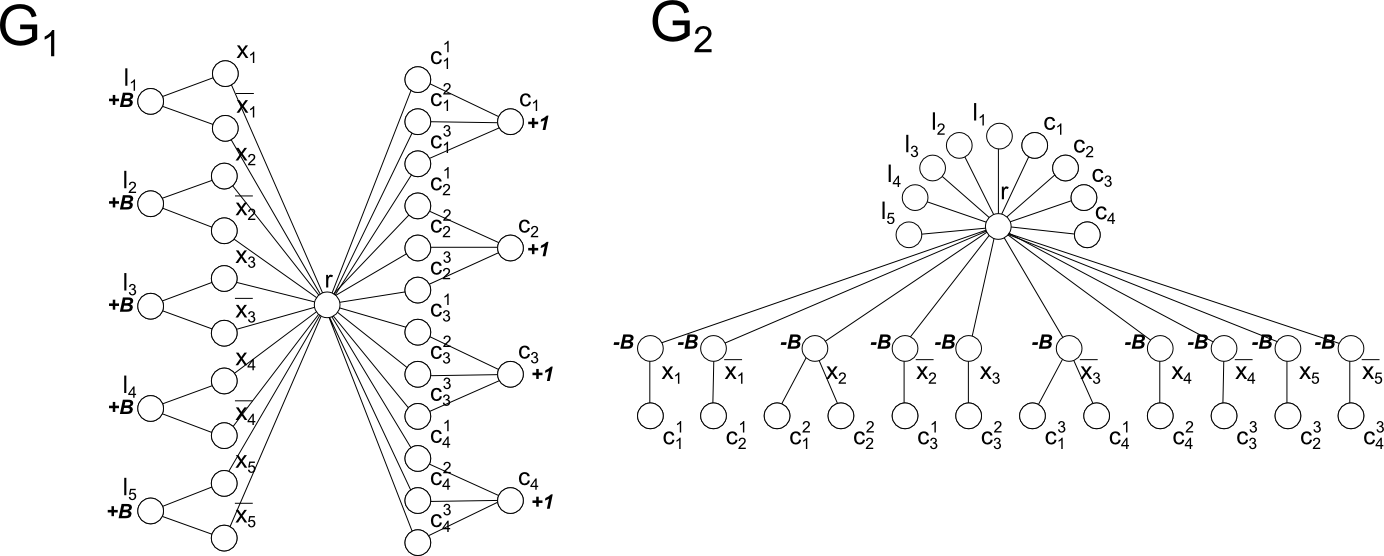
\includegraphics[width=\textwidth]{apx_g-tree}
    	 	 \caption{XXX refaire avec TikZ si temps le permet XXX Illustration of the construction of $G_1$, $G_2$, and $M$, given $C_q = \{(x_1 \vee x_2 \vee \neg{}x_3), (\neg{}x_1 \vee x_2 \vee x_5), (\neg{}x_2 \vee x_3 \vee \neg{}x_4), (\neg{}x_3 \vee x_4 \vee \neg{}x_5)\}$. For readability, the mapping $M$ is not drawn but deduced from the labels of the nodes; any pair of nodes (one in $G_1$ and one in $G_2$) of similar label are mapped in $M$.}\label{fig:g-tree}
    	 	 \end{figure}
   		
		Let us prove that this construction is indeed an L-reduction from \msat{}. More precisely, we prove the following property.

		\begin{lemma}
 	 	 There exists an assignment of $V_n$ satisfying at least $m$ clauses of $C_q$ if and only if there exists a solution (not necessarily optimal) to \mwccs{} of weight at least $m$.
		\end{lemma}

		\begin{proof}

		{\parindent0pt
		$\boxed\Rightarrow$} Given an assignment $\mathcal{A}$ of $V_n$ satisfying $m$ clauses of $C_q$, we construct a solution to \mwccs{} of weight $m$ as follows.

		Let $V_1^*=V_2^*=\{c_j~\vert~ c_j \text{ is satisfied by } \mathcal{A}\} \cup \{c^k_j~\vert~ c^k_j \text{ is satisfying } c_j \text{ by } \mathcal{A}\}\cup\{x_i~\vert~ x_i=1\}\cup\{\overline{x_i}~\vert~ x_i=0\}\cup \{r,l_i~\vert~ 1\leq i\leq n\}$. 

		By construction, $G_1[V_1^*]$ and $G_2[V_2^*]$ are connected. Moreover, $G_1[V_1^*]$ contributes $B\times n+m$ to the overall weight of the solution, that is $B$ for each of the $l_i$ and $+1$ for each satisfied clause, while $G_2[V_2^*]$ contributes $-B\times n$ to the overall weight of the solution since exactly one of each variable node ($i.e.$, $x_i$ and $\overline{x_i}$) has been kept. The overall solution is valid and of total weight $m$.

		\vspace*{1em}
		{\parindent0pt
		$\boxed{\Leftarrow}$} Given any solution $V^*\subseteq V_1$ to \mwccs{} of weight $m$, we construct a solution to the \msat{} problem satisfying at least $m$ clauses as follows.

		First, note that, as in the previous construction, we can assume that any such solution to \mwccs{} is \textit{canonical} meaning that $V^*$ does not contain both vertices $x_i$ and $\overline{x_i}$ for any $1\leq i\leq n$.

		Let $\mathcal{A}$ be an assignment of $V_n$ such that for all $1\leq i\leq n$, if $x_i\in V^*$ then $x_i=1$ and $x_i=0$ otherwise. Note that, since our solution is canonical, each literal has been assigned a single boolean value in $\mathcal{A}$. Let us now prove that this assignment satisfies at least $m$ clauses of $C_q$.

		First, note that since our solution is canonical, as in the previous construction, the weight $m$ of the solution can only be induced by $m$ clause nodes of $G_1$, say $\mathcal{C}_1\subseteq V^*$.

		Since both $G_1[V^*]$ and $G_2[V^*]$ have to be connected, any solution with $m>1$ will include node $r$ in $V^*$. Thus, for each node $c_j\in\mathcal{C}_1$ there should be a node of $\{c_j^k ~\vert~ 1\leq k\leq 3\}$ in $G_1[V^*]$ to connect $c_j$ to $r$. In $G_2[V^*]$, in order for nodes $r$ and $c_j^k$ to be connected, the corresponding literal node (that is $x_i$ or $\overline{x_i}$), say $x_i$ -- has to be kept in $V^*$. By construction, this is the case if $x_i$ is the $k$-th literal of clause $c_j$. Thus, $\mathcal{A}$ is an assignment that satisfies any clause $c_j$ such that the clause node $c_j$ belongs to $V^*$. As already stated $|\mathcal{C}_1|=m$.
		\end{proof}

		The above reduction linearly preserves the approximation and proves \cref{prop:apx-t-graph}.

		\subsubsection{Binary tree and graph}
		\label{subsubsec:binary-tree}

		XXX refaire si temps le permet XXX

	\section{Polynomial-time cases for the \mwccs{} problem}
	\label{sec:poly}

		\subsection{Two bounded-degree trees and a bijective mapping}
		\label{subsec:tree1o1}

			Here we continue to explore the case with fixed $\alpha = 1$.
			We have proved in \cref{subsec:apx-bt-cater} that for instances with two binary trees, and an injective mapping function, the problem is APX-hard.
			We will now consider the case of two bounded-degree trees, $T_1 = (V_1, E_1)$ and $T_2 = (V_2, E_2)$, with a bijective relationship, or mapping function, $V_1\,M\,V_2$. Without loss of generality, lets now suppose that their respective degrees are $d_{T_1} = d_{T_2} = d$, and that $\norm{V_1} = \norm{V_2} = n$.

%			The standard algorithms for \mwcs{} and its variants\footnote{Mainly cardinality-constrained, budget-constrained, and ratio-bounded, with a pseudo-polynomial algorithm for all of them exposed in the next chapter.} use bottom-up, usually dynamic-programming, approaches.
%			Given an unrooted tree $T$, root $T$ in one of its node to direct the edges.
%			Then, compute recursively the maximum weight of the subtrees that unconditionally includes their root.

%			It would be a good characteristic of our algorithm to advance in a similar fashion, recursively solving subproblems, and progressing in both trees in locked step.
			Since $\alpha=1$, a node can only be selected if its counterpart is also selected.
			However, note that a node in one of the trees %\footnote{With any arbitrary node as its root.}
			can have its counterpart at a completely different depth in the other tree %\footnote{Also with any arbitrary node as its root.}
			 (see \cref{fig:childReqParent}).
			Consequently, adding a child node might require the addition of a parent by mutual requirement between the two trees and the mapping function (see \cref{fig:childReqParent}).
			This exhibit the main difficulty with this problem: the non-isomorphic mapping function makes it impossible to use the usual local dynamic programming scheme to solve the \mwcs{} problem and its variants on trees.

			\begin{figure}[ht]
				\centering
            \begin{tikzpicture}[level/.style={sibling distance=10em/#1},
              every node/.style = {shape=circle, draw, align=center}]]
              \node {R}
                child { node {A}
                  child { node {\phantom{N}} }
                  child { node {\phantom{N}} }
                }
                child { node {C}
                  child { node {\phantom{N}} }
                  child { node {B} }
                };
            \end{tikzpicture}
            \qquad
            \begin{tikzpicture}[level/.style={sibling distance=10em/#1},
              every node/.style = {shape=circle, draw, align=center}]]
              \node {r}
                child { node {b}
                  child { node {a} }
                  child { node {c} }
                }
                child { node {\phantom{N}}
                  child { node {\phantom{N}} }
                  child { node {\phantom{N}} }
                };
            \end{tikzpicture}

%				\includegraphics[width=\textwidth,height=0.3\textwidth]{childReqParent.png}
				\caption[Caption for LOF]{Nodes labeled with the same letter are counterpart of one another.
				
				When starting from an empty solution\protect\footnotemark, the inclusion of node $A$ requires only the inclusion of $a$. However when starting from the root nodes, the inclusion of node $A$ requires the inclusion of node $a$, which recursively requires the inclusions of $b$, $B$, $C$, and $c$.
			
				A local dynamic programming approach is impossible since the context is important.}
				\label{fig:childReqParent}
			\end{figure}

			In this section, we introduce a \emph{functional dynamic programming} approach for this setup that solve the \mwccs{} problem in polynomial time parameterized on the degree of the trees. A functional dynamic programming approach is a \emph{top-down} dynamic programming technique, that is recursive and using subproblem overlaps, that uses a \emph{memoization} scheme to store intermediate results instead of the usual tabular approach.

			Our algorithm is composed of two main operations.
			$\text{ComputeDecisionTree}$ is the main functionnal dynamic programming procedure and finds the optimal solution to the problem given two trees and a root for one of them.
			$\text{ComputeDecisionTree}$ calls upon $\text{ConstructRequiredSet}$ to maintain the connectivity and matching constraints of the candidate solution.
			%Now the complete operations might seem unnecessarily complex for now, but will become self-explanatory in the end.

			\footnotetext{As is the case with regular dynamic programming, which depend only on local subproblems.}

			\paragraph{$\text{ConstructRequiredSet}$:}
			Informally, $\text{ConstructRequiredSet}$ takes as input all the nodes that have been included up intil now, from both $T_1$ and $T_2$, and add into those sets all nodes that are required to be added if $u$ is included to keep 1) connectivity and 2) perfect matching (see \cref{fig:childReqParent}).

			Adding a node $u \in V_1$ from $T_1$ to a candidate solution\footnote{At least one of the neighbors of $u$ is in the candidate solution, or the candidate solution is empty. That is, its addition leaves the candidate solution connected.} requires the unconditional inclusion of its counterpart $v \in V_2$ from $T_2$ to the candidate solution.
			In turn, the addition of $v$ requires the addition of all nodes from $T_2$ that are necessary for the candidate solution to remain connected: the (possibly empty) shortest path $v_0 v_1 \ldots v_i$ between $v$ and, if one exists, its closest node from $T_2$ already in the solution.
			Recursively, this requires the addition of all counterparts of the nodes $v_0$, $v_1$, $\ldots$, $v_i$ to the candidate solution, and the nodes required for the candidate solution to remain connected.
			This recursion continues until no more nodes are required to be included to conserve connectivity.

			It is formally defined as follows.
			Given two sets $S_1 \subseteq V_1$ and $S_2 \subseteq V_2$ of nodes already selected, and a node $u \in V_1 \setminus S_1$ such that $u$ is a neighbor of a node in $S_1$ ($v \in V_2$ its counterpart).
			We define a double recursion procedure over $V_1$ and $V_2$.
			Add $u$ to $S_1$; then, find the shortest path from its counterpart $v$ to any node of $S_2$.
			Add all nodes that pertain to this shortest path to $S_2$ (including $v$), and recursively find all shortest paths from their counterparts to the nodes of $S_1$.
			%Note that since the graphs are trees, the order which is used to call the procedure on all these nodes can be arbitrary.
			Continue until no more nodes need to be added.

			\begin{proposition}\label{prop:constructFuncConnected}
				The induced graphs $T_1[S_1]$ and $T_2[S_2]$ obtained as results of $\text{ConstructRequiredSet}$ are connected.
			\end{proposition}
			\begin{proof}
				Indeed, since we recursively add nodes with their shortest path to already selected nodes, there exists a path connecting every pairs of nodes of $S_1$ and of $S_2$.
			\end{proof}

			\begin{proposition}\label{prop:constructFuncQuadratic}
				$\text{ConstructRequiredSet}$ is a quadratic operation in the worst case.
			\end{proposition}
			\begin{proof}
				The shortest path toward a set of nodes in a tree is equivalent to the minimum sum subsequence problem and can be solved in linear time using a dynamic programming approach.
				We recursively add up to $O(n)$ nodes (all).
				Hence the resulting complexity.
			\end{proof}

			\paragraph{$\text{ComputeDecisionTree}$:}
			The main procedure, $\text{ComputeDecisionTree}$,  is a recursive decision tree traversal of $T_1$ that uses the $\text{ConstructRequiredSet}$ operation.
%			This recursive procedure, $\text{ComputeDecisionTree}$ is formally defined as follows.
%			Given two sets $S^u_1$ and $S^u_2$ of connected nodes in $V_1$ and $V_2$ respectively, and a node $u$: the last selected node in the decision tree.
%			Lets define $u^i$ the $i$-th children of $u$, and $C_u = \bigcup\limits_i{u^i}$ the set of these children. %, and $C = C_u \setminus S_1$ the children of $u$ that where not added to $S_1$ in any of the previous decisions.
%			%If all children of $u$ have been recursively added at the previous step ($C = \emptyset$), end this branch of the decision tree.
%			%If $u$ has not children ($C = \emptyset$), end this branch of the decision tree.
%			For all nodes $u^i \in C_u$, if any:
%			\begin{enumerate}
%				\item call the $\text{ConstructRequiredSet}$ procedure with $S^u_1$, $S^u_2$, and $u^i$, which will return $S^{u_i}_1$ and $S^{u_i}_2$, and
%				\item recursively expend the decision tree by calling $\text{ComputeDecisionTree}$ with $S^{u_i}_1$, $S^{u_i}_2$, and $u^i$.
%			\end{enumerate}
%			We then compute a score $s(S_1, S_2, u)$ for this node (defined by the selection of $u$ in the decision tree) as follows.
			It is formally defined as follows.
			Given $T_1$, $T_2$, and a node $u \in V_1$, this function returns the set $S^u_1$ and $S^u_2$: the best selection of nodes, respectively from $T_1$ and $T_2$, when optimizing in the subtree rooted in $u$ and which includes $u$.
			Note that $S^u_1$ might contain nodes that are parents to $u$, as a requirement for the matching and connectivity constraints.
			Lets define $u_i$ the $i$-th children of $u$, and $C^u = \bigcup\limits_i{\{u_i\}}$ the set of these children. %, and $C = C_u \setminus S_1$ the children of $u$ that where not added to $S_1$ in any of the previous decisions.
			%If all children of $u$ have been recursively added at the previous step ($C = \emptyset$), end this branch of the decision tree.
			%If $u$ has not children ($C = \emptyset$), end this branch of the decision tree.
			For all nodes $u_i \in C^u$, if any:
			\begin{enumerate}
				\item recursively call $\text{ComputeDecisionTree}$ with $u_i$, which will return the sets $S^{u_i}_1$ and $S^{u_i}_2$, then
				\item call the $\text{ConstructRequiredSet}$ procedure with $S^{u_i}_1$, $S^{u_i}_2$, and $u$, which will return $\accentset{\circ}{S^{u_i}_1}$ and $\accentset{\circ}{S^{u_i}_2}$.
			\end{enumerate} 
			Then compute a score $s(u)$, which correspond to the optimal combination of children such that their inclusion maximizes the local sum of weights.
			This score only consider the subtree rooted in $u$ and including $u$ in a typical dynamic programming approach.

			Formally, the computation of this score is as follows.
			For notation sake, lets define $\mathcal{P}^u = \mathcal{P}\left({C^u}\right)$: the \emph{power set} containing all the combinations of children of $u$; and $\mathcal{P}^u_k$ the $k$-th element of this set.
			Lets also define $S^{\mathcal{P}^u_k} = \bigcup\limits_{u^i \in \mathcal{P}^u_k}{\accentset{\circ}{S^{u_i}_1} \cup \accentset{\circ}{S^{u_i}_2}}$: the union of the optimal nodes in the $k$-th combination of children\footnote{Note that in general, this union is certainly not optimal. Unless there are multiple optimal solutions, only one combination of the children maximizes the score, and possibly the empty one.}, including $u$.
			To simplicity notation, we further define $S^{\mathcal{P}^u_0}$, with the $0$-th combination being the usual empty set\footnote{Here of children.}, as the set $\{u, v\}$: if no children are selected, only the current node and its counterpart are part of the solution, which is a connected and matched solution by definition.
			Finally, we have:
%			\[
%				w(S^{d_i}) = w(n_i) + \max\left(0, w\left(S^{{\langle r\rangle}_{d_i}}\right), w\left(S^{{\langle r\rangle}_{d_i}}\right), w\left(S^{{\langle l\rangle}_{d_i}} \cup S^{{\langle r\rangle}_{d_i}}\right)\right)
%			\]
%			\[
%			s(u) = w(u) + \max\left(\begin{array}{c}
%				0,\\
%				w\left(S^{{\langle \text{left}\rangle}_{d_i}}\right),\\
%				w\left(S^{{\langle \text{right}\rangle}_{d_i}}\right),\\
%				w\left(S^{{\langle \text{left}\rangle}_{d_i}} \cup S^{{\langle \text{right}\rangle}_{d_i}}\right)
%			\end{array}\right)
%			\]
%			\begin{align*}
%				s(u)
%					& = \sum\limits_{n \in S^u}{w(n)} + \max\limits_{k}{\left(0, \sum\limits_{n \in S^{\mathcal{P}^u_k} \setminus S^u}{w(n)}\right)} \\
%					& = \max\limits_{k}{\left(\sum\limits_{n \in S^u}{w(n)}, \sum\limits_{n \in S^{\mathcal{P}^u_k}}{w(n)}\right)}
%			\end{align*}
			\[
				s(u) = \max\limits_{k}{\sum\limits_{n \in S^{\mathcal{P}^u_k}}{w\left(n\right)}}
			\]

			Computing the optimal combination of children, required for the $\max$ function, is not an easy problem.
			It looks similar to the \textsc{weighted maximum coverage} problem \parencite{hochbaum1996approximation}, relaxed both with possibly negative weights, and with unconstrained number of sets.
			It also looks quite similar to the \textsc{set-union knapsack} problem \parencite{goldschmidt1994note}, but again with real-valued weights and without budget constraint.
			Both are sensibly related and difficult, NP-hard problems~\parencites{hochbaum1996approximation,cohen2008generalized}.
			However, since we are working with bounded-degree trees, the number of combinations remains (parameterized-)constant. The overall algorithm is thus in FPT (Fixed-Parameter Tractable), see \cref{prop:decisionTreeComplexity} for proof.

			\begin{proposition}
				$\text{ComputeDecisionTree}$ is a parameterized complexity algorithm which requires at most $O(2^d n^2 + n^3)$ steps for $d$-ary trees.
				\label{prop:decisionTreeComplexity}
			\end{proposition}
			\begin{proof}
				The recursion tree closely follows the topology of $T_1$, and contains at most $O(n)$ calls.
				At each step we use the $\text{ConstructRequiredSet}$ procedure, which is a quadratic time operation.
				We also compute the score, which itself requires to compute a set union operation for each combination of children.
				There are at worst $O(2^d)$ combination of children (the cardinality of the power set), and set union is at worst an $O(n)$ operation with a bitvector representation of the sets.
				Hence the resulting number of steps.
			\end{proof}

%			\paragraph{}
%			Overall, note that this procedure construct increasingly inclusive set of required nodes $S_1$ and $S_2$.
%			This is expected, since recursive calls can only add nodes to the solution in order to maintain the two connectivity and matching contraints after each decision.
%			However, it effectively defines an environment into which the recursive $\text{ComputeDecisionTree}$ operate, implicitly defined by the initial node and the set of choices made up until the current node.
%
%			
%
%			\begin{figure}[ht]
%				\centering
%				\includegraphics[width=\textwidth,height=0.3\textwidth]{DecisionTreeWithScores.png}
%				\label{fig:foo}
%			\end{figure}
%
%			We thus need to iterate this decision tree procedure for all pairs $u,v \in V_1\times V_2$.

			\begin{proposition}
				One of the recursive calls of $\text{ComputeDecisionTree}$ contains the optimal solution to the global problem.
			\end{proposition}
			\begin{proof}
				Even though two subtrees could actually have the exact same solution, since parent nodes can be included for matching and connectivity constraint reasons, it should be clear from the standard tree traversal that the whole tree $T_1$ is considered and that all its subtrees (that respect the constraints) are evaluated.
				To see that the optimal solution found by this procedure, in $T_1$, is also the optimal in regard to $T_2$, note that any given subtree of $T_1$, that is valid under the constraints, have one and only one counterpart subtree in $T_2$.
				Indeed, since the matching is a bipartite function, each node have one and only one counterpart; any subtree of size $m$ in $T_1$ have one and only one counterpart subtree of size $m$ in $T_2$, the one that contains all counterpart nodes.
				Finally, since all possible subtrees of $T_1$ (that respect the constraints) are considered, it must be that all possible subtrees of $T_2$ are also considered by this procedure.
			\end{proof}

			The optimum is in the recursive call with the highest total score, the optimal objective, and the optimal solution is the corresponding set of nodes $S^u$.

%			\begin{proposition}\label{prop:totalComplex}
%				The overall algorithm to compute the optimal solution is an $O(n^3)$ running time algorithm.
%			\end{proposition}
%			\begin{proof}
%				Indeed, since the nodes are on a one to one mapping, there exists exactly $n = \norm{V_1} = \norm{V_2}$ pairs of nodes $u,v \in V_1\times V_2$.
%				For each such pair we call $\text{ComputeDecisionTree}$ which is an $O(n^2)$ operation.
%
%				In the end, the optimal solution is in one of the $O(n^3)$ decision tree nodes.
%
%				Hence the total running time.
%			\end{proof}

		\subsection{Polynomial-time scheme for some inputs}
		\label{subsec:enumerable}

			Here we consider the general version of the \mwccs{} problem where $\alpha$ is given as input rather than being fixed.
			In addition, we further relax the constraint on the relationship function, which can be any partial injective function.
			That is, any element of $V_1$ can have at most one image in $V_2$ (the elements of $V_2$ can have 0, 1, or more antecedents).
			Finally, we suppose that there is a polynomial number of connected induced subgraphs of $G_1$.

			We consider as many candidate solution as there are connected subgraphs of $G_1$, and for each one of them we try to find the best corresponding subgraph in $G_2$.
			The best corresponding subgraph in $G_2$ is the subgraph that maximizes the total weight of the candidate solution and such that at least an $\alpha$-fraction of the nodes of $G_1$ and $G_2$ in the solution are $M$-related.
			For a given subgraph of $G_1$, the sum of its nodes' weight is fixed, hence maximizing the total weight of the candidate solution is equivalent to finding the optimal solution in $G_2$ where the $\alpha$-fraction constraint holds.

			To solve this problem, we introduce a new problem, the \textsc{ratio-bounded maximum-weight connected subgraph} (\rbmwcs) problem.
			Informally, it consists in a variant of the \mwcs{} problem where an additional contribution function is associated to each node and where an additional ratio constraint is introduced\footnote{not unlike the \emph{budget-constrained} variant of the \mwcs{} problem}, formally defined in \cref{subsubsec:foo}.

			The reduction to this new subproblem is as follows.
			The contribution function needs to \emph{encode} the relationship function between the nodes of both $G_1$ and $G_2$.
			To do so, and since we fixed a partial solution to the problem in the form of the subgraph of $G_1$, we note for each node of $G_2$ its number of inverse images in $G'_1$ plus one if and only if at least one exists, zero otherwise.
			The reason we need to make the distinction between the two cases is that when there is no counterpart in $G_1$, selecting a node in the optimal solution in $G_2$ will not increase the number of mapped node overall.
			However, selecting a node in $G_2$ for which there exists at least one counterpart will increase the number of mapped node by the number of counterpart, plus one for the selected node itself.

			Formally, given a connected subgraph $G'_1=(V'_1,E'_1)$ of $G_1$, we define the corresponding $G_2$ \emph{antecedent function} $a\colon V_2 \to \mN$ to be $a(v)=\card{\Set{v,u}{M(u,v), u\in V'_1}}$.
			The \emph{contribution function} $c\colon V_2 \to \mN$ is defined as follows:
			$$c(v)=\begin{cases}a(v) + 1 &\mbox{if }a(v) > 0\mbox{,} \\
		                       0        &\mbox{otherwise.}
		          \end{cases}$$

			Given $G_2=(V_2,E_2)$, its weight-function $w_2$ and its contribution function $c$, the problem now corresponds to the discovery of the connected subgraph of maximum weight such that:
			\begin{align*}
				\sum_{v \in V^*_2}{c(v)}                           &\geq \alpha\times\left(\norm{V'_1} + \norm{V^*_2}\right) \\
				\sum_{v \in V^*_2}{c(v)} - \alpha\times\norm{V'_1} &\geq \alpha\times\norm{V^*_2}
			\end{align*}
			Where $\alpha\times\norm{V_1'}$ is constant.

			Finally, given the optimal score of all candidate solutions, for which there are one for each subgraphs $G'_1$, the optimal solution to the \mwccs{} problem is the one candidate solution among them which has the best score.

			Clearly, constructing a contribution function for $G_2$ given a subgraph $G'_1$ is a linear time operation.
			Choosing the best candidate solution is as time consuming as enumerating all subgraphs of $G_1$, which is a polynomial time operation in this context.
			The complexity of this algorithm hence depends on the difficulty to solve the \rbmwcs{} subproblem.

			\Cref{sec:rbmwcs} provides an analysis of this problem with a more general contribution function.
%			It provides pseudo-polynomial scheme for all classes of input graphs up to bounded treewidth.
			It provides polynomial scheme for $d$-ary trees and an optimized algorithm for paths.
%			However, when the contribution function is enumerable with a polynomial upper bound, and such is the case by construction here, the scheme actually becomes a polynomial-time algorithm.
%			Thus, there exists a polynomial-time algorithm to solve \mwccs{} when one of the graph if polynomially enumerable, the second is bounded treewidth, and the relationship is a partial injective function, for any $\alpha \in [0, 1]$.
			Thus, there exists a polynomial-time algorithm to solve \mwccs{} when one of the graph if polynomially enumerable, the second is a bounded-degree tree, and the relationship is a partial injective function, for any $\alpha \in [0, 1]$.

	\section{The Ratio-Bounded Maximum-Weight Connected Subgraph problem}
	\label{sec:rbmwcs}

		In this section, we introduce a slightly more general version than required in \cref{subsec:enumerable}\footnote{The contribution function can represent inputs that we don't actually use.}.
		The \textsc{ratio-bounded maximum-weight connected subgraph} (\rbmwcs) problem, is formally defined as follows.

		\textbf{\rbmwcs{}}: Given a node-weighted graph $G = (V, E)$, its node-weighting function $w\colon V \to \mR$, its contribution function $c\colon V \to \mR$, a ratio $\alpha \in [0,1]$ and a constant $C \in \mR$, find a subset $V^* \subseteq V$ such that:
			\begin{enumerate}
				\item the induced graph $G\left[V^*\right]$ is connected, and
				\item the ratio of the sum of contributions plus some constant over the number of nodes in the solution is greater than or equal to $\alpha$, that is:\\
					$\sum\limits_{v \in V^*}{c(v)} + C \geq \alpha\times\card{V^*}$, and
				\item $\sum\limits_{v \in V^*}{w(v)}$ is maximum.
			\end{enumerate}

		\begin{proposition}
			\rbmwcs{} is at least as difficult as \mwcs{}.
		\end{proposition}
		\begin{proof}
			Indeed, when $c(v) = 1,\,\forall v\in V$, the ratio $\sum\limits_{v \in V^*}{c(v)} / \card{V^*} = 1 \geq \alpha$, and the \mwcs{} and \rbmwcs{} problems are equivalent.
		\end{proof}

		Let us show now that it is in PTIME for bounded-degree trees.
		\begin{proposition}
			\rbmwcs{} is solvable in $O(n^{d+2})$ time for $d$-ary trees.
			\label{prop:boundedDegreeTreesRBMWCS}
		\end{proposition}
		\begin{proof}
			Let us consider the \rbmwcs{} problem for a $d$-ary tree.
			We define a dynamic programming strategy with a $O(n^{d+2})$ time complexity.
			This leads to a polynomial algorithm for $d$-ary trees.
			The basic idea is to define a 3-dimensional table $T$ of size $\card{V}\times \sum_{v\in V}c(v) \times \card{V}$ that stores the maximum weight of a subtree rooted in $v$ of size $s$ and of total contribution $tc$.

			Formally, $\forall v\in V,\,0 \leq tc \leq \sum_{v\in V}c(v),\,0 \leq s \leq |V|$, let us note $v_{\langle i\rangle}$ the $i$-th child of $v$, $1 \leq i \leq d$, we have:
			% \[
			%   \begin{array}{rl}
			%   	T[v][0][0]   &= 0 \\
			%     T[v][tc][s]  &= \mathlarger{\max}_{tc_1,\ldots,tc_d,\,\,s_1,\ldots, s_d}\left(w(v) +
			%                         \mathlarger{\sum}_{1 \leq i \leq d}{T[v_{\langle i\rangle}][tc_i][s_i]}
			%                     \right) \\
			%                  & \vphantom{foo} \\
			%     s.t.\quad tc &= c(v) + \mathlarger{\sum}_{1 \leq i \leq d}{tc_i} \\
			%               s  &= 1    + \mathlarger{\sum}_{1 \leq i \leq d}{s_i}
			%   \end{array}
			% \]

			\[
			  \begin{array}{rl}
					T[v][0][0]   &= 0 \\
				  T[v][tc][s]  &= \max\limits_{tc_1,\ldots,tc_d,\,\,s_1,\ldots, s_d}\left(w(v) +
											 \sum\limits_{1 \leq i \leq d}{T[v_{\langle i\rangle}][tc_i][s_i]}
										\right) \\
									& \vphantom{foo} \\
				  s.t.\quad tc &= c(v) + \sum\limits_{1 \leq i \leq d}{tc_i} \\
								s  &= 1    + \sum\limits_{1 \leq i \leq d}{s_i}
				\end{array}
			\]

			The optimal subtree can be reconstructed from the table by finding the entry with the maximal weight and where the contribution ratio is not violated, and backtracking from that entry on the selected $tc_i$'s and $s_i$'s from the $\max$ function.
			Each entry of the table can be computed in $O(n^{d-1})$ (that is, an integer partition of $\card{V}$ into $d$ parts) time, and since $\sum_{v\in V}c(v) \in O(n)$, there are $O(n^3)$ of them, which leads to the overall complexity.
		\end{proof}

		As paths and cycles are trees of degree $1$, using the preceding result leads to an $O(n^3)$ algorithm for these cases. However, one can achieve a better complexity.

		\begin{proposition}
		  \rbmwcs{} is solvable in $O(n^2)$ time for paths and cycles.
		\end{proposition}
		\begin{proof}
			Let us first consider the \rbmwcs{} problem for paths. Leveraging the linearity of the graph structure, we define a dynamic programming strategy with an $O(n^2)$ time complexity.

			The idea is to define two 2-dimensional tables $T_w$ and $T_{tc}$ with $n^2$ entries each and that store respectively, for each pair of indices, the maximum weight and the total contribution, of the corresponding graph. Let us consider a given orientation in the path with the node at the starting end as the reference node, of index 0. Every candidate solution (a subpath) in the path can then be defined as a pair of positions, the first element being the starting position as an index number, the second element being the size of the candidate solution. The main idea being that increasing the indices one by one enables us to update the weights and total contributions incrementally.

			Formally, let us denote the $k$-th node of the graph in the predefined orientation by $n_k$, we have for all $0 \leq i \leq j \leq n$: 
			\[
			  \begin{array}{rl}
				T_w[i][i]    &= 0 \\
				 T_w[i][j]    &= w(n_{i+j-1}) + T_w[i][j-1] \\
				 \vphantom{foobar} \\
				 T_{tc}[i][i] &= 0 \\
				 T_{tc}[i][j] &= c(n_{i+j-1}) + T_{tc}[i][j-1]
			  \end{array}
			\]

			The optimal subpath is defined by the indices of the entry with the maximal weight and where the contribution ratio is not violated ($i.e.$, for any $(i,j)$ s.t. $T_{tc}[i][j]\geq \alpha \cdot j$).
			Each $O(n^2)$ entry of the tables can be computed in constant time, leading to the overall complexity.
			For cycles, the trick consists in taking any linearization of the cycle and merging two copies of the corresponding linearization as the input path.
			This ensures that we will consider any candidate solution ($i.e.$, simple subpath of the cycle).
			The time complexity is preserved.
		\end{proof}


	\section{Related questions and further work}

		In this contribution we provide the first deep complexity analysis of the \mwccs{} problem, but there still remains a fair number interesting problems and questions.

		First of all, generalizing the problem to more than two graphs is of practical interest.
		It seem that the most general expression of the problem is to have a, possibly empty, mapping function between each graph.
		However, as we've shown throughout this chapter, the mapping function is a most important factor in the complexity of the problem.
		It is expected that the FPT algorithm for $d$-ary trees would remain in such complexity category when generalized to $k$ trees and $\frac{k(k+1)}{2}$ bijective mappings, but formal proof remains to be done.
		By generality of the problems, the hardness results for two graph will hold with more graphs.
		However it is unclear whether the polynomial-time solvable cases would remain so, and if that is the case with which polynomial exponent.

		Studying the effects of a relaxation of the connectivity constraints in \mwccs{} would be quite interesting.
		The problem would then become similar to the \textsc{set-union knapsack}, with a bipartite partition of the sets, and where the maximum weight becomes a moving target ($\alpha$-ratio).

		In \cref{subsec:enumerable} we effectively presented a reduction from some instances of \mwccs{} to instances of \rbmwcs{}.
		There exists trivial reduction from \rbmwcs{} to \mwccs{}.
		However, whether \mwccs{} is more general than \rbmwcs{} and can encode any of its instances remains an open question.

		Interestingly, analyses of the links between \rbmwcs{} and the variants of \mwcs{}, such as the budget constraint one, is an already ongoing direction of research.
		Indeed, the ratio constraint $\sum\limits_{v \in V^*}{c(v)} + C \geq \alpha\times\card{V^*}$ of the \rbmwcs{} problem is a generalization of the costs constraint $\sum\limits_{v \in V^*}{\text{cost}(v)} \leq B$ of the \bcmwcs{} problem\footnote{Observe that $\sum\limits_{v \in V^*}{c(v)} + C \geq \alpha\times\card{V^*} \Leftrightarrow \sum_{v \in V^*} (c(v) - \alpha) \geq -C$.}.
		Since \rbmwcs{} is effectively a more general variant than the \textsc{budgeted \mwcs{}} problem, which is itself a more general variant of the \textsc{cardinality-constrained \mwcs{}} problem, itself a more general variant of \mwcs{}, all algorithms that apply to \rbmwcs{} also apply to the others.

		Going in this direction, instead of the \emph{integer partition} enumeration scheme used in \cref{prop:boundedDegreeTreesRBMWCS}, we can probably use a tabular dynamic programming approach quite similar to \textsc{knapsack} where the weights are actually contributions.
		It would effectively remove the degree bound for the trees and make the algorithm pseudo-polynomial.
		Finally, preliminary results suggest that this dynamic programming solution to the subproblems of \rbmwcs{} could actually be introduced in the algorithm that \textcite{bateni2011prize} introduced, making a pseudo-polynomial algorithm for \rbmwcs{} for all graphs up to bounded-treewidth.

\chapter{The Ratio-Bounded MWCS}
\label{chap:rbmwcs}

	In this chapter, XXX explain XXX.

	A slightly more general version\footnote{the contribution function is more expressive here} of the problem introduced at the end of the previous chapter is called the \textsc{ratio-bounded maximum-weight connected subgraph} (\rbmwcs) problem, and in the general case is defined formally as follows.

	\textbf{\rbmwcs{}}: Given a node-weighted graph $G = (V, E)$, its node-weighting function $w\colon V \to \mR$, its contribution function $c\colon V \to \mR$, a ratio $\alpha \in [0,1]$ and a constant $C \in \mR$, find a subset $V^* \subseteq V$ such that:
	\begin{enumerate}
		\item the induced graph $G\left[V^*\right]$ is connected, and
		\item the ratio of the sum of contributions plus some constant over the number of nodes in the solution is greater than or equal to $\alpha$, that is:\\
			$\sum\limits_{v \in V^*}{c(v)} + C \geq \alpha\times\card{V^*}$, and
		\item $\sum\limits_{v \in V^*}{w(v)}$ is maximum.
	\end{enumerate}

	\begin{proposition}
		\rbmwcs{} is as difficult as \mwcs{}.
	\end{proposition}
	\begin{proof}
		Indeed, when $\forall v\in V, c(v) = 1$, the ratio $\sum\limits_{v \in V^*}{c(v)} / \card{V^*} = 1 \geq \alpha$, and the \mwcs{} and \rbmwcs{} problems are equivalent.
	\end{proof}

	\section{A more general variant of the \textsc{budget-constrained mwcs}}
		The \textsc{budget-constrained maximum-weight connected subgraph}, also named the \textsc{budgeted mwcs} (\bcmwcs{}) is formally defined as follow.
		
		\textbf{\bcmwcs{}}: Given a node-weighted graph $G = (V, E)$, its node-weighting function $w\colon V \to \mR$, its cost function $\text{cost}\colon V \to \mR^+$, and a budget $B \in \mR^+$, find the subset $V^* \subseteq V$ such that:
		\begin{enumerate}
			\item the induced graph $G\left[V^*\right]$ is connected, and
			\item the sum of the costs does not exceed the allocated budget $B$, that is:\\
				$\sum\limits_{v \in V^*}{\text{cost}(v)} \leq B$, and
			\item $\sum\limits_{v \in V^*}{w(v)}$ is maximum.
		\end{enumerate}

		Note that appart from the cost and ratio constraints, the two problems are stricly equivalent.

		\begin{proposition}
			The ratio constraint $\sum\limits_{v \in V^*}{c(v)} + C \geq \alpha\times\card{V^*}$ of the \rbmwcs{} problem is a generalization of the costs constraint $\sum\limits_{v \in V^*}{\text{cost}(v)} \leq B$ of the \bcmwcs{} problem.
		\end{proposition}

		\begin{proof}
			\begin{align*}
				\sum\limits_{v \in V^*}{c(v)} + C &\geq \alpha\times\card{V^*} \\
				\sum\limits_{v \in V^*}{c(v)} + C &\geq \sum\limits_{v \in V^*}{\alpha} \\
				\sum\limits_{v \in V^*}{c(v)} - \sum\limits_{v \in V^*}{\alpha} &\geq -C \\
				\sum\limits_{v \in V^*}{c(v) - \alpha} &\geq -C \\
				\sum\limits_{v \in V^*}{\alpha - c(v)} &\leq C \\
				\sum\limits_{v \in V^*}{c'(v)} &\leq C \\
			\end{align*}

			The range of the function $c'$ is a superset of the range of the function $\text{cost}$ since the later is positive.
			The same argument is made for \bcmwcs{}'s constant $B$ which is positive where the constant $C$ is real.
		\end{proof}

		\begin{proposition}
			There exists a linear reduction from \bcmwcs{} to \rbmwcs{} problem, hence the latter is more general.\qed{}
		\end{proposition}

		\begin{proof}
			Given an \bcmwcs{} problem,
			\begin{enumerate}
				\item the graph $G = (V, E)$ do not change, neither does the weight function $w$,
				\item define the cost function $c(v) = \alpha - \text{cost(v)},\,\,\forall \alpha \in [0,1]$, and
				\item the constant $C = B$.
			\end{enumerate}
			This defines a suitable reduction from \bcmwcs{} to \rbmwcs{}.
		\end{proof}


	\section{Pseudo-polynomial algorithms from \mwcs{}}

		XXX Argument about the reasoning with $c\colon V \to \mZ$ instead of $c\colon V \to \mR$, which 1] is valid for our reduction in chap 4 and 2] holds for \bcmwcs{} XXX

		\subsection{Explicit algorithms for trees and cactii}

		\subsection{For bounded treewidth graphs}


\bookmarksetup{startatroot}
\cftinserthook{toc}{UnindentChap}
\chapter{Conclusion}
%\addcontentsline{toc}{chapter}{Conclusion}
%\chaptermark{Conclusion}
\label{chap:concl}




\backmatter
\pagenumbering{alph}

\printbibliography

\end{document}
